\chapter[The Pebble Bed Fluoride-Salt-Cooled High-Temperature Reactor]{The Pebble Bed Fluoride-Salt-Cooled High-Temperature Reactor}
\chaptermark{The Pebble Bed FHR}
\label{sec:pbfhr}

% I'd have an introductory sentence at the least that frames this chapter, potentially a paragraph. 
Throughout most of the history of the \gls{pbr} concept, helium has been the working fluid of choice \cite{claxton,hecker,oehme,nrc_avr,moormann,thtr_1990,hofmann,thomas,koster,gao,chen_htr,xu_htr,htrpm}. Helium has low neutron interaction cross sections, a thermal conductivity several times larger than other common gases \cite{gases_k}, and is chemically compatible with fuel and structural materials. 

In the past 20 years, considerable interest has grown in the use of molten salt coolants for \glspl{pbr}. The volumetric heat capacities of molten salts, like most liquids, are two to three orders of magnitude higher than those of gases at the same temperature and pressure. Even when pressurized to tens of atmospheres, the lower volumetric heat capacity of gas-cooled systems limits them to power densities two to three orders of magnitude smaller than liquid-cooled systems. Power density often directly translates to the structural material inventory, which contributes roughly 10\% of the overnight capital cost of construction \cite{xin_wang_thesis}. Atmospheric pressure systems also eliminate many complex pressurizing systems, further reducing cost.

The early development of gas-cooled systems emphasized high outlet temperatures needed for process heat applications. While the initial goal of a sustained 1000\si{\celsius} outlet temperature has in most gas-cooled designs been reduced to the 750\si{\celsius} range due to material limitations, the high boiling points of molten salts enable operation at similar temperatures as gas-cooled systems while retaining the operational simplicity associated with single-phase flow. High temperature operation also corresponds to higher thermal efficiency. 

To place these statements in a more quantitative perspective, Fig.\ \ref{fig:fluid_T_p} shows characteristic primary loop operating pressure and core outlet temperature for reactor designs based on five different coolants\mdash water in a \gls{bwr}, water in a \gls{pwr}, sodium in a fast reactor, carbon dioxide in an \gls{agr}, helium in a \gls{htgr}, \gls{flibe} in a \gls{htr}, and an organic oil in an organic-cooled reactor\hspace{0.02cm}\footnote{Water in a \gls{scwr} is not included because the extreme changes in thermal properties with temperature and pressure at and beyond the critical point make calculation of a meaningful average \(\rho_fC_{p,f}\) difficult.}. The area of each circle is proportional to the volumetric heat capacity \(\rho_fC_{pf}\) of each coolant at the average operating temperature and pressure. 

\begin{figure}[h!]
\centering
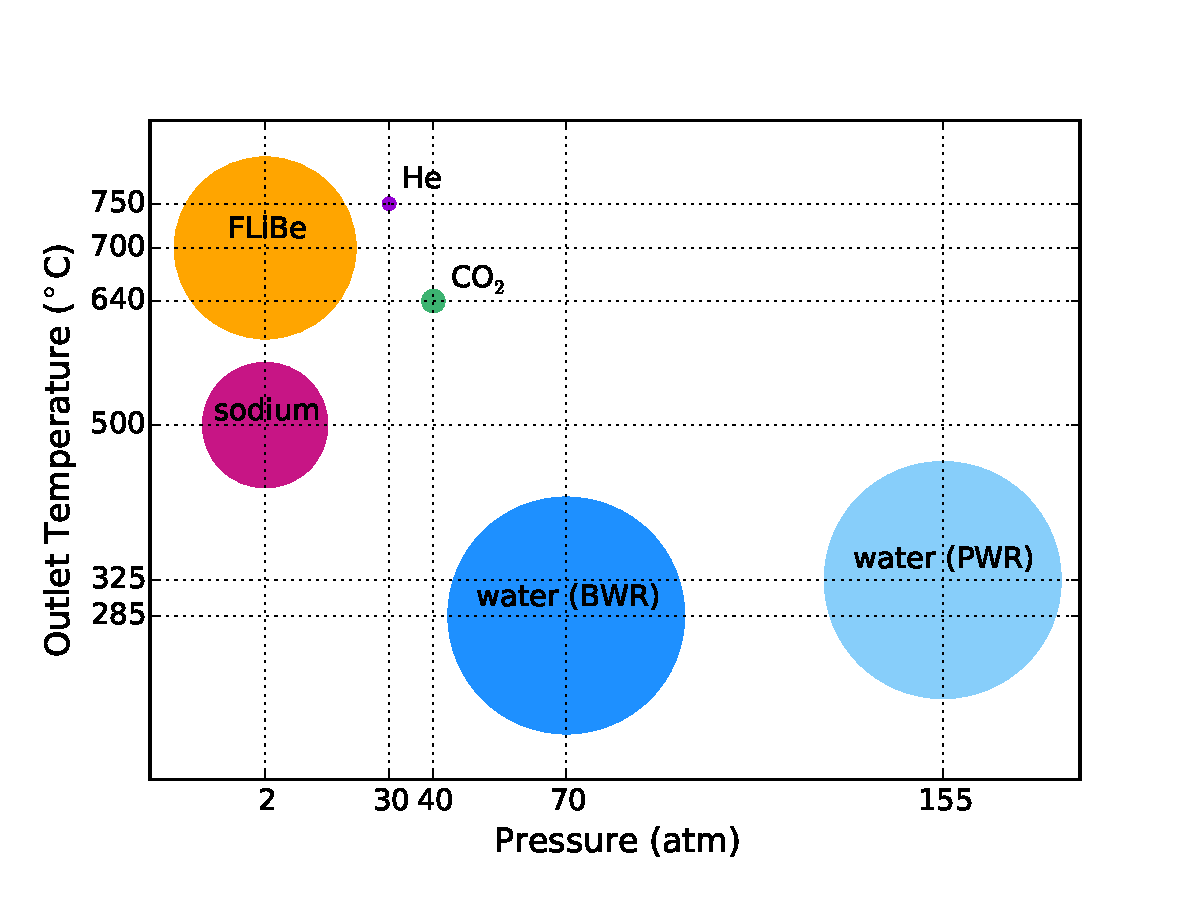
\includegraphics[width=0.6\linewidth]{figs/fluid_T_p.pdf}
\caption{Characteristic pressure and outlet temperature for reactor designs based on five common coolants. The area of each circle is proportional to \(\rho_fC_{p,f}\).}
\label{fig:fluid_T_p}
\end{figure}

Salt-cooled designs can operate at similar outlet temperatures as many helium-cooled \glspl{pbr} and carbon dioxide cooled \glspl{agr} without significant pressurization. Water coolants require significant pressurization to reach relatively low outlet temperatures with sufficient heat removal capabilities; to the author's knowledge, water coolants have only been proposed for a fluidized bed concept introduced in Chapter \ref{sec:intro} \cite{sefidvash,sefidvash_1996}.

Most chemically pure molten salts are compatible with common structural materials such as nickel alloys and graphite \cite{fratoni}. Lubrication of graphite in salt is also expected to result in significantly less graphite dust production from frictional pebble wear than in helium-cooled \glspl{pbr}. Further, many fission products are soluble in molten salts. Through proper fission product cold trap design, salt-cooled systems may exhibit a more predictable source term than gas systems, simplifying both accident analyses and decommissioning activities \cite{moormann}.

The selection of reactor coolant is always a balance between many design objectives that include efficiency, reliability, safety, and economics. Molten salts have relatively high freezing points, in the vicinity of 450 to 500\si{\celsius}; extensive trace heating systems are required to prevent salt freezing and flow blockages. And while salts such as \gls{flibe} contribute to neutron moderation \cite{fratoni}, the high \((n,^3\text{H})\) absorption cross section in $^6$Li requires enrichment of the lithium in lithium-bearing salts from a natural $^7$Li concentration of 92.41\% to high purities, typically 99.995\%, to ensure a negative coolant temperature coefficient and acceptable tritium production rates. The lack of significant infrastructure results in an uncertain cost associated with $^7$Li enrichment. The design of \gls{flibe}-cooled \glspl{pbr} in particular often includes additional constraints on minimizing coolant inventory to reduce cost \cite{pbfhr}.

The multiscale model described in Chapter \ref{sec:PhysicalModels} applies to all single-phase \glspl{pbr}. Chapter \ref{sec:sana} presented validation of the friction-dominated macroscale model to depressurized conduction cool-down in gas-cooled \glspl{pbr}. At the time of writing, a lack of experimental data for salt-cooled \glspl{pbr} precludes a similar validation for salt systems. Therefore, in lieu of validation exercises, this section demonstrates application of the multiscale model to full-core, steady-state analysis of a salt-cooled \gls{pbr} considering the pebble bed, outer reflector bypass, and conjugate heat transfer with structural materials. 

The objectives of this section are to 1)~assess the capability of the multiscale model for capturing physics important to salt-cooled \glspl{pbr}; 2)~describe the incorporation of high-resolution \gls{cfd} into the coarse-mesh multiscale model for closure generation; and 3)~predict the core \gls{th} of a salt-cooled design of current interest to the Nuclear Engineering department at \gls{ucb}\mdash the Mark-1 \gls{pbfhr}. 

This particular concept design is selected for application of the multiscale models developed in this dissertation because several aspects of the core design both highlight model and implementation strengths relative to ``legacy'' \gls{pbr} simulation tools and constitute significantly different \gls{th} conditions than seen in most helium-cooled \glspl{pbr}. For example, a combination of radial and axial inflow \glspl{bc} results in multi-dimensional core flow, rather than the ``plug'' flow typically observed in helium-cooled \glspl{pbr}. The interaction of these non-uniform flow \glspl{bc} with non-Cartesian inflow and outflow boundaries necessitates unstructured meshing capabilities. 

An unconventional reflector block design with strong coupling between horizontal and vertical flow channels requires generation of new drag closures with off-line \gls{cfd} modeling. The pebble design is also distinct from the gas-cooled design shown in Fig.\ \ref{fig:pbr_fuel}. A very thin fuel-matrix annulus, as opposed to a large central heterogeneous core, may cause the \gls{hl} method to perform poorly because of thermal resistance distortion. The \gls{hsd} verification performed for compacts in Chapter \ref{sec:vv} may also not extend to thin regions, especially when considering the ad hoc averaging and extrema approximations in Eqs. \eqref{eq:MaxT}--\eqref{eq:AvgT}.

This section also incorporates many additional physical phenomena that are often omitted in preliminary analyses of salt-cooled designs. In place of a simple volume average of the phase thermal conductivities \cite{xin_wang_thesis,scarlat}, inter-pebble stagnant conduction, contact conduction, and radiation are included. And while the increase in advective heat transfer due to thermal dispersion is usually neglected \cite{xin_wang_thesis,scarlat}, this ``braiding'' effect is considered. Likely more significant than the inclusion of additional macroscale physics is the addition of bypass flow modeling. A lack of reflector drag closures prevented earlier studies from accounting for the reduction in core cooling associated with core bypass, resulting in non-conservative maximum fuel temperature predictions.

The remainder of this section is organized as follows. Section \ref{sec:mark1} describes the Mark-1 \gls{pbfhr} design, revisiting in greater detail the features highlighted in the preceding paragraphs. Section \ref{sec:pbfhr_model} describes the computational model of the Mark-1 \gls{pbfhr} core. To determine the applicability of the \gls{hsd} and \gls{hl} methods to fuel designs with thin fuel-matrix annuli, Section \ref{sec:meso_fhr} compares the \gls{hsd} and \gls{hl} fuel models against reference, explicitly-resolved, \gls{pbfhr} pebbles. To enable full-core modeling incorporating bypass flow, Section \ref{sec:bypass} describes the generation of drag correlations for the outer reflector blocks at end-of-life using COMSOL Multiphysics. Several gap sizes are investigated to identify the sensitivity of core undercooling to reflector block lifetime. 

Section \ref{sec:core} then combines the macroscale model described in Section \ref{sec:macro_deriv}, the meso and micro scale models described in Section \ref{sec:mesomicro} and verified in Section \ref{sec:meso_fhr}, and the high-resolution reflector block closure generation discussed in Section \ref{sec:bypass} to full-core steady-state analysis of the Mark-1 \gls{pbfhr}. Section \ref{sec:inflow} evaluates several potential core-flow \glspl{bc} from the perspective of the bypass fraction, outlet fluid temperature distribution, and pumping power. For a number of different reflector block gap distributions, an inflow \gls{bc} design that achieves low bypass, pressure drop, and maximum outlet temperatures is recommended for more detailed analysis.

Section \ref{sec:depth} then provides predictions of pressure; velocity; and fuel, coolant, and structural material temperatures for the coupled pebble bed and reflector system with the inflow \gls{bc} developed in Section \ref{sec:inflow}. Finally, Section \ref{sec:conclusions_fhr} revisits the limitations of the present work and outlines next steps in improving multiscale models for salt-cooled \glspl{pbr}.

\section{The Mark-1 Design}
\label{sec:mark1}

The Mark-1 \gls{pbfhr} is a 236 MWth \gls{flibe}-cooled \gls{pbr} concept developed by \gls{ucb}, \gls{mit}, and \gls{uw} through a \gls{doe} \gls{irp} \cite{pbfhr}. The combination of a high boiling point and low vapor pressure coolant with a robust pebble fuel form enables high-temperature and atmospheric pressure operation with passive decay heat removal. This section introduces the reactor design features salient for multiscale \gls{th} analysis in Sections \ref{sec:meso_fhr}--\ref{sec:core}. All geometric, operational, and material descriptions of the \gls{pbfhr} are taken from a technical design report published in 2014 by the \gls{th} Lab at \gls{ucb} \cite{pbfhr}. For brevity, the ``Mark-1'' designation is dropped throughout this section.

The nominal operating conditions of the \gls{pbfhr} relevant to core thermal analysis are summarized in Table \ref{table:operating}. The core consists of fixed block-type inner and outer graphite reflectors that constrain the pebbles into an annulus. Fig.\ \ref{fig:pbfhr_core} shows an illustration of the pebble bed region and a crude representation of the inner reflector. Conceptual streamlines are hand-drawn as gray lines; flow into the outer reflector is not shown.

\begin{table}[htb!]
\caption{Nominal operating conditions of the \gls{pbfhr}.}
\centering
\small
\begin{tabular}{|l|c|}
\hline\hline
Operating Condition & Value\Tstrut\Bstrut\\
\hline
Thermal power & 236 MWth\Tstrut\\
Total mass flowrate & 976 \si{\kilo\gram\per\second}\\
Inlet temperature & 600\si{\celsius}\\
Outlet temperature & 700\si{\celsius}\\
Outlet pressure & 2 atm\Bstrut\\
\hline
\end{tabular}
\label{table:operating}
\end{table}

Surrounding the pebble bed is an outer graphite reflector, which is successively enclosed in a stainless steel 316 core barrel, a thin coolant downcomer region, and a stainless steel 316 reactor vessel. A \gls{rrcls} consisting of 0.5 \si{\meter} thick insulating firebrick liner blocks within a water-cooled reactor cavity liner plate reduce parasitic heat losses while ensuring sufficient heat removal in \glspl{bdbe}. The cavity liner plate is nominally maintained at 30\si{\celsius} to protect the thick layer of concrete encasing the \gls{rrcls}. Thermal properties for stainless steel, firebrick, and reflector graphite are provided in Appendix \ref{sec:props}.

Fig.\ \ref{fig:pbfhr_core2} shows a \gls{cad} rendering of the reactor vessel internals with the inner reflector mostly withdrawn from the top of the core and the bed region vacated of pebbles. Not shown are the firebricks, \gls{rrcls} system, and concrete that successively enclose the reactor vessel.

\begin{figure}[h!]
    \begin{subfigure}{0.5\linewidth}
        \centering
        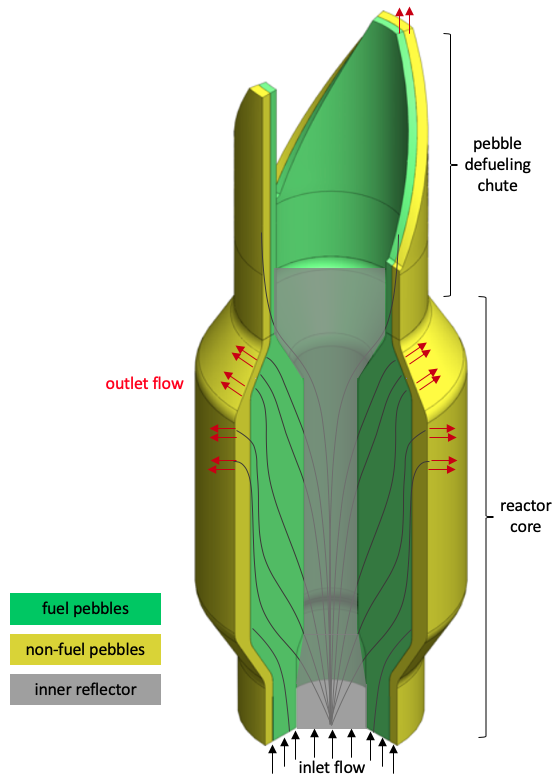
\includegraphics[height=1.1\linewidth]{figs/pbfhr_core.png}
       \caption{Pebble bed and inner reflector}
       \label{fig:pbfhr_core}
    \end{subfigure}
    \begin{subfigure}{0.5\linewidth}
        \centering
        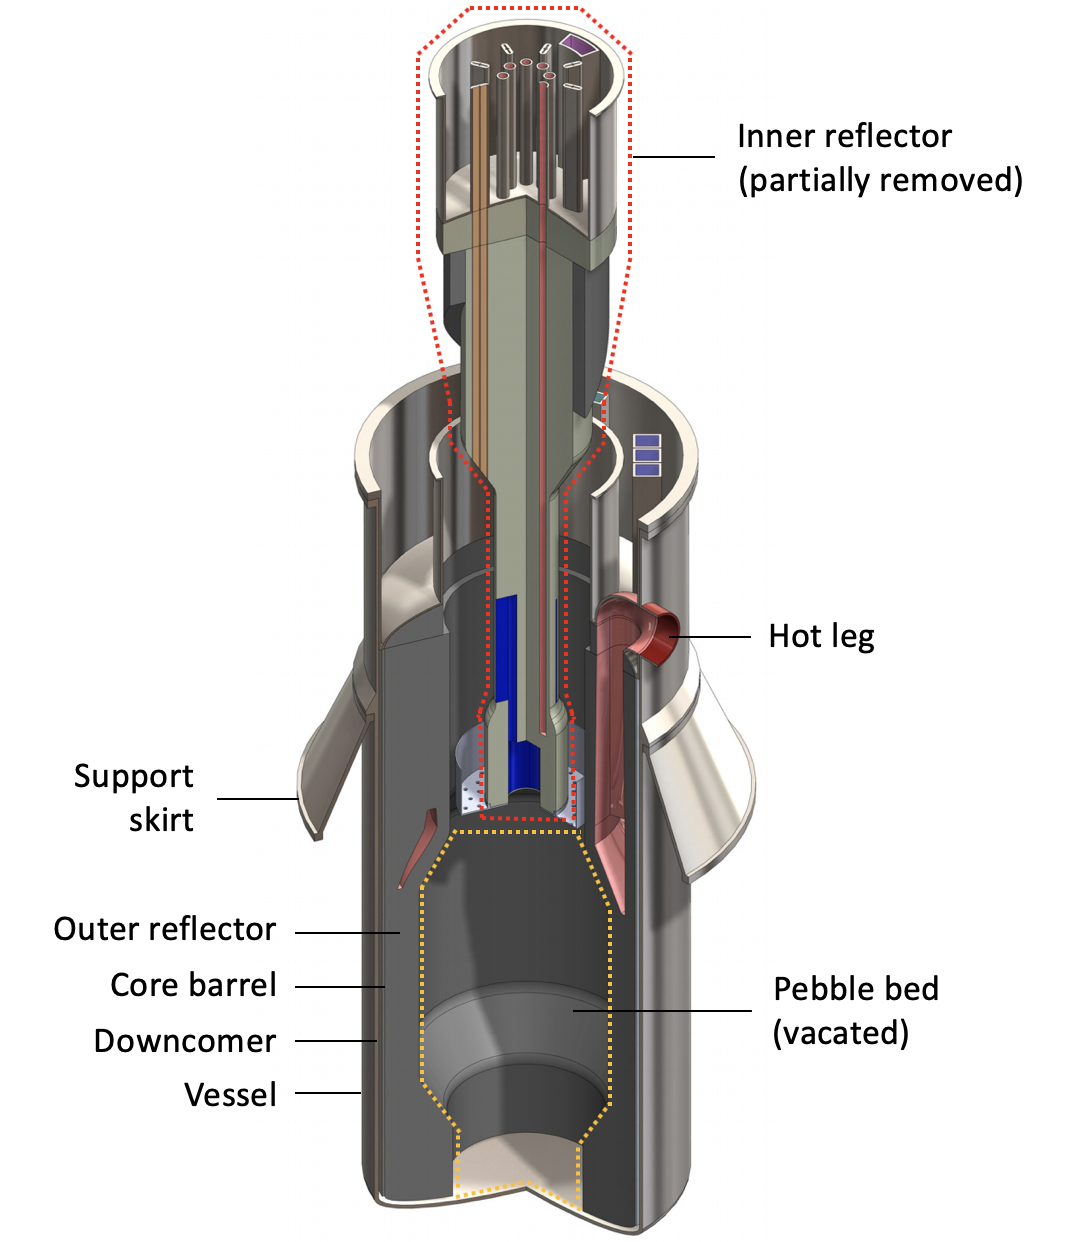
\includegraphics[height=1.1\linewidth]{figs/pbfhr_cad_core.png}
        \caption{Reactor vessel internals}
        \label{fig:pbfhr_core2}
    \end{subfigure}
    \caption{Schematic of the \gls{pbfhr} (a) pebble bed region with conceptual streamlines drawn in gray and (b) reactor vessel internals (adapted from \cite{pbfhr, krumwiede}).}
    \label{fig:pbfhr_big}
\end{figure}

\gls{flibe} enters the downcomer from two cold legs and then flows upwards directly into the pebble bed, the outer reflector, and through a series of machined channels in the central reflector. Fig.\ \ref{fig:in} shows a \gls{cad} model of one of the stacked blocks comprising the inner reflector at the core axial mid-plane. Each block is 0.26 \si{\meter} tall and consists of eight control rod channels and 16 instrumentation channels. Coolant flows upwards through the eight ``teardrop''-shaped channels and the eight control rod channels, entering the bed through horizontal slots between lobes and through the 20 coolant suction holes on each lobe, of which only five are indicated on the bottom lobe in Fig.\ \ref{fig:in}. 70\% of the total flow enters the bed through the central reflector, while the remaining flow is split between the pebble bed and the outer reflector according to the bypass flow fraction, or the fraction of the total flow that enters the outer reflector. 

In most \gls{pbr} designs, the coolant flow is primarily axial, lacking major inlet flow paths originating in the reflectors. Radial flow results in a lower core pressure drop than purely axial flow because the fluid path length through the bed is reduced. 

\begin{figure}[h!]
\centering
\hspace{1.1cm}
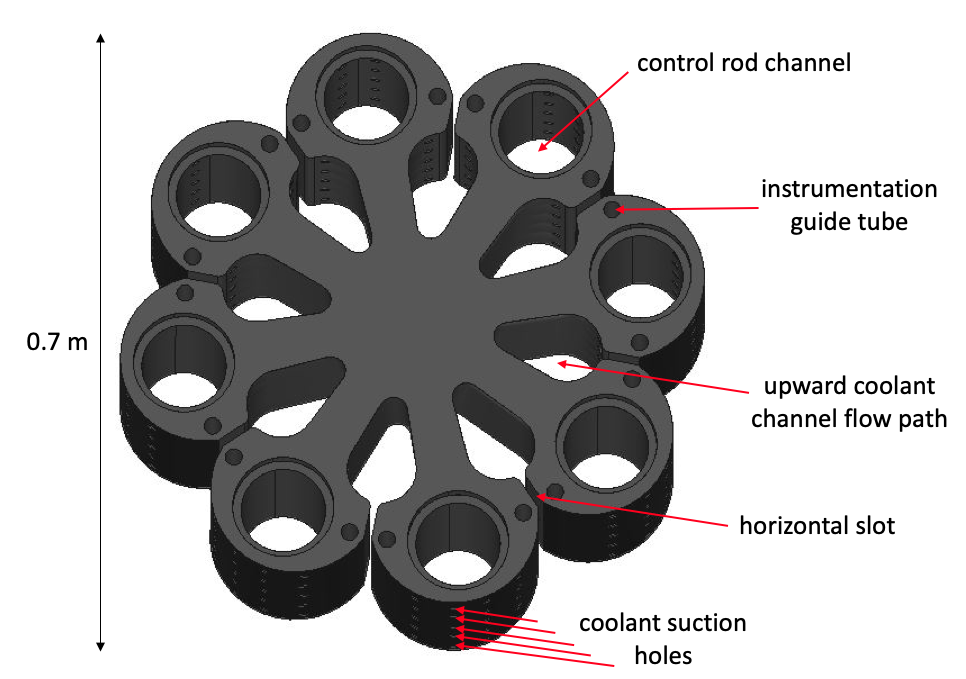
\includegraphics[width=0.5\linewidth]{figs/center_reflector_labeled.png}
\caption{Schematic of one of the stacked inner reflector blocks at the core mid-plane of the \gls{pbfhr} with various channels and flow paths indicated.}
\label{fig:in}
\end{figure}

The \gls{flibe} leaves the pebble bed through the defueling chute at the top of the core and through a series of axisymmetric suction holes on the inner surface of the outer reflector that connect to a single hot leg. The coolant from the defueling chute and the hot leg is then mixed in a collection plenum before transport to a power conversion system.

The outer reflector is constructed as rings of stacked graphite blocks; there are 24 blocks per ring. Fig.\ \ref{fig:ring} shows a \gls{cad} model of one ring of blocks, while Fig.\ \ref{fig:block} shows a close-up view of a single block. Each block contains a vertical coolant channel that is connected to the bed by 24 horizontal suction holes. Grooves on the back of each block fit into ribs on the core barrel to maintain alignment. The \gls{pbfhr} outer reflector block design differs from that in most gas-cooled \glspl{pbr} because the presence of horizontal suction channels leads to a strong coupling between horizontal and vertical flows.

\begin{figure}[h!]
    \begin{subfigure}{0.5\linewidth}
        \centering
        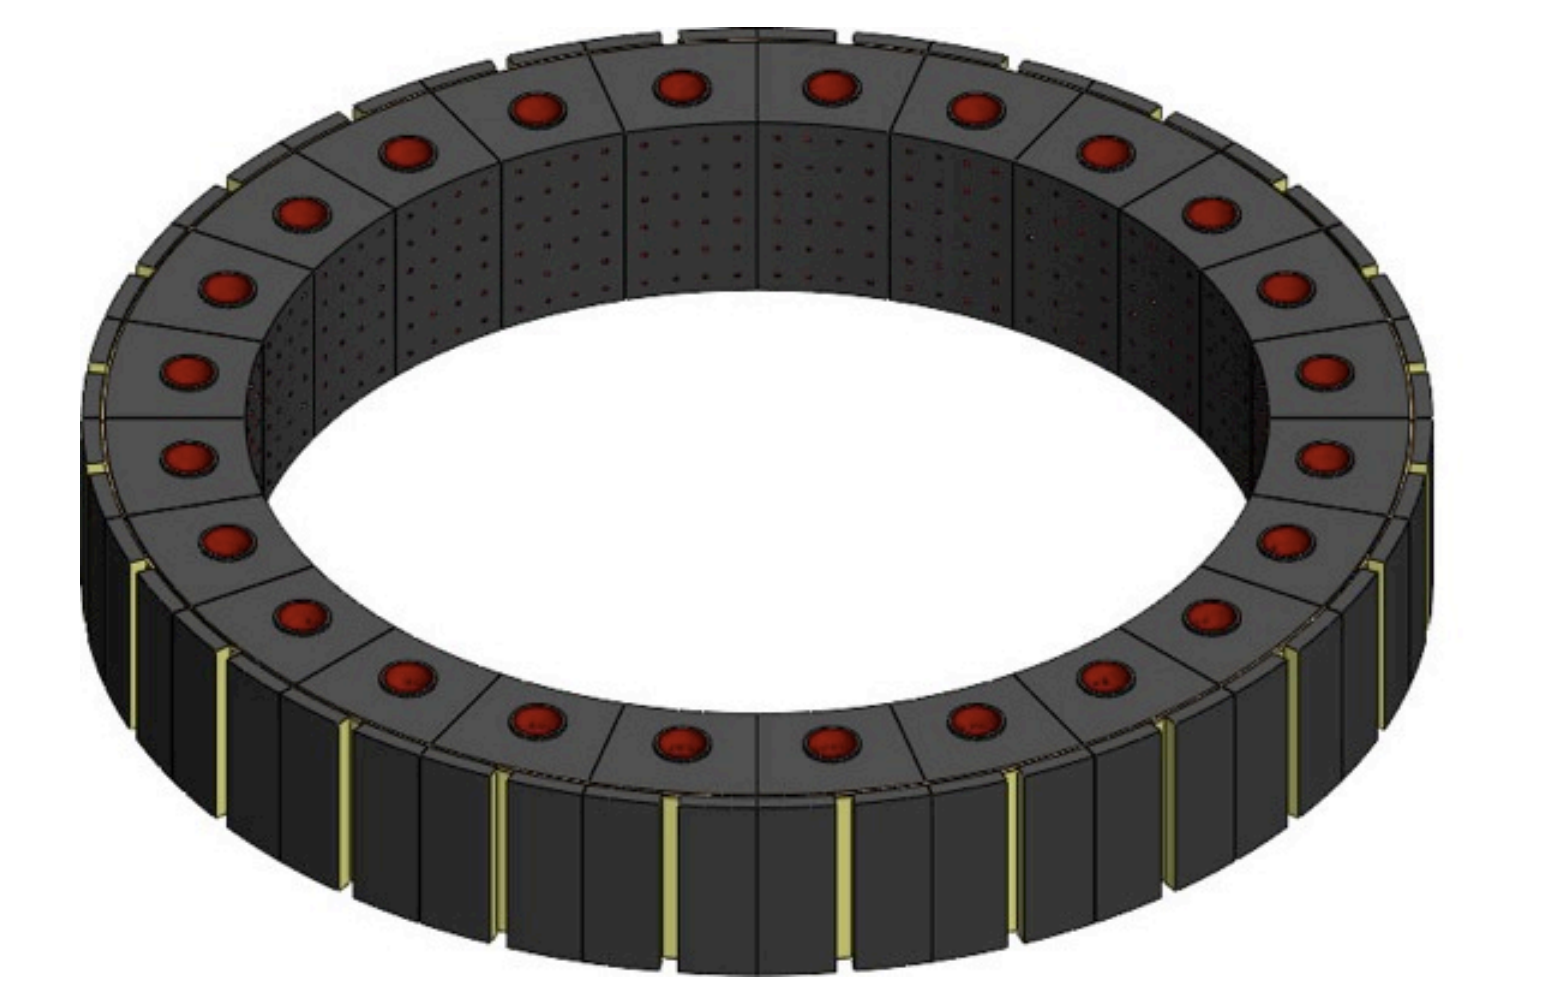
\includegraphics[height=0.6\linewidth]{figs/or_ring.png}
       \caption{Ring of outer reflector blocks}
       \label{fig:ring}
    \end{subfigure}
    \begin{subfigure}{0.5\linewidth}
        \centering
        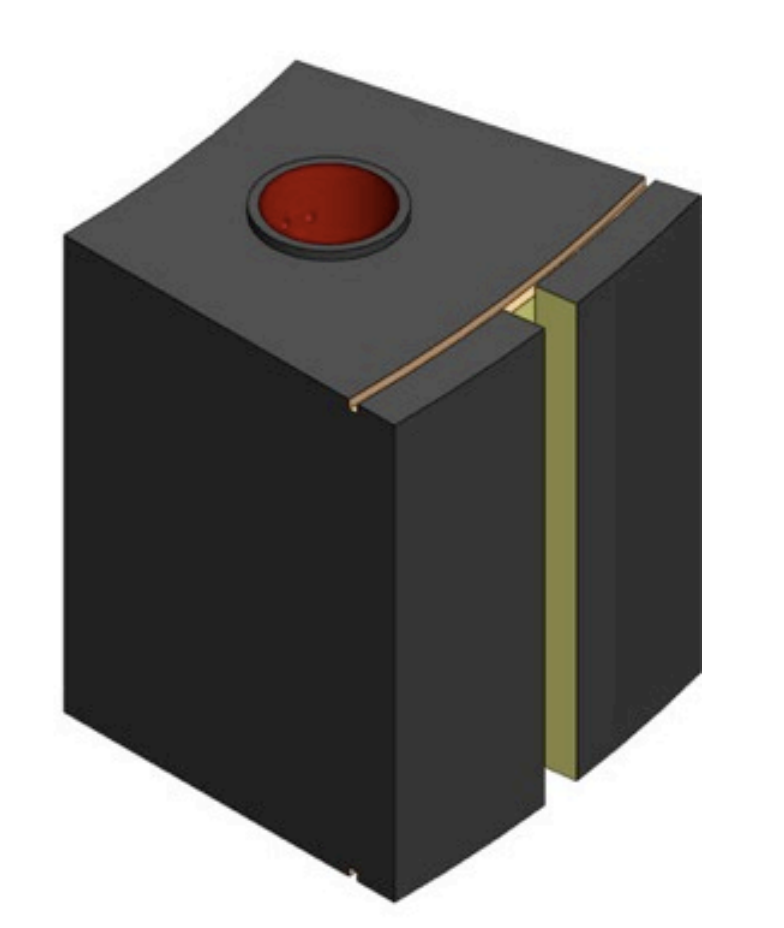
\includegraphics[height=0.6\linewidth]{figs/or_block.png}
        \caption{Close-up view of single reflector block}
        \label{fig:block}
    \end{subfigure}
    \caption{Schematic of the \gls{pbfhr} outer reflector (a) ring and (b) block \cite{pbfhr}.}
    \label{fig:pbfhr_ring}
\end{figure}

The core contains two different types of 3 \si{\centi\meter} diameter pebbles\mdash fuel pebbles and non-fueled graphite blanket pebbles. Approximately 470,000 fuel pebbles comprise the majority of the bed, while approximately 218,000 graphite pebbles are located in a thin region adjacent to the outer reflector to protect the outer reflector from fast fluence. These two regions are shown as ``fuel pebbles'' and ``non-fuel pebbles'' in Fig.\ \ref{fig:pbfhr_big}. 

The \gls{pbfhr} fuel pebble differs from the nominal gas-cooled pebble design introduced in Section \ref{sec:pbr_concept}. To allow higher power densities without exceeding integrity temperature limits, the fuel-matrix region occupies a thin annular shell near the pebble surface instead of a large central core, a concept that has been considered since the very early days of \glspl{pbr} \cite{claxton}. The fuel pebbles consist of three regions\mdash 1)~a central graphite core with an outer radius of 1.2 \si{\centi\meter}; 2)~a heterogeneous fuel-matrix region with 30.9\% \gls{pf} of \glspl{cfp} in a graphite matrix with a thickness of 0.2 \si{\centi\meter}; and 3)~an outer graphite shell with a thickness of 0.1 \si{\centi\meter}. 

The density of the center graphite core is selected such that the total pebble density is 84\% of the coolant density at average operating conditions to ensure neutral buoyancy \cite{fratoni}. The \gls{cfp} uses the standard \gls{triso} particle design. The \gls{cfp} consists of a central UC$_{1.5}$O$_{0.5}$ fissile kernel successively enclosed by a porous graphite buffer, an inner \gls{pyc} layer, a \gls{sic} layer, and an outer \gls{pyc} layer. A schematic of a fuel pebble with randomized particle coordinates obtained using the OpenMC Monte Carlo code is shown in Fig.\ \ref{fig:pbfhr_fuel} \cite{romano}. Colors indicate the different material regions, with a legend on the right.

\begin{figure}[h!]
\centering
\hspace{1.5cm}
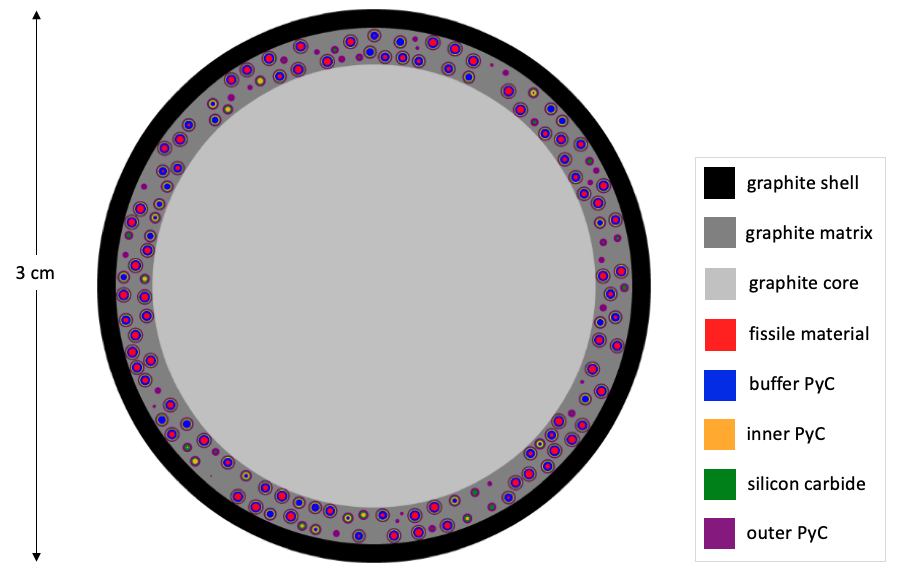
\includegraphics[width=0.6\linewidth]{figs/pbfhr_pebble.png}
\caption{Schematic of a \gls{pbfhr} fuel pebble along a slice through the center of the pebble with random particle coordinates obtained from the OpenMC Monte Carlo code \cite{romano}.}
\label{fig:pbfhr_fuel}
\end{figure}

The present analysis assumes a slightly thicker fuel-matrix shell thickness than the nominal design in order to fit the specified number of \glspl{cfp} given the constraint that particles cannot intersect the boundaries of the shell. The use of a thicker fuel-matrix region also meets realistic minimum inter-particle separation distances required to attain low as-manufactured defect fractions when using overcoating fabrication methods \cite{morris,nabielek,minato}. The geometry of the fuel particles and the pebble thermal properties are given in Table \ref{table:pebble_props}. Constant properties are selected based on evaluating the temperature-dependent correlations in Appendix \ref{sec:props} at the expected operating temperature. Finally, the pebble emissivity, Poisson ratio, and elastic modulus are assumed to be 0.8, \(9\times10^9\) Pa, and 0.136, respectively \cite{baker}.

\begin{table}[htb!]
\caption{Properties and kernel geometry for the \gls{pbfhr} fuel pebble \cite{novak_manual}.}
\centering
\small
\centerline{
\begin{tabular}{|l| c c c |c|}
\hline\hline
Material & \(\rho_S\) (\si{\kilo\gram\per\cubic\meter}) & \(k_S\) (\si{\watt\per\meter\per\kelvin}) & \(C_{p,S}\) (\si{\joule\per\kilo\gram\per\kelvin}) & Outer Radius in CFP (\si{\micro\meter})\Tstrut\Bstrut\\
\hline
UC$_{1.5}$O$_{0.5}$ & $11000$ & $\color{white}0\color{black}3.5$ & $\color{white}0\color{black}400$ & $200$\Tstrut\\
Porous carbon & $\color{white}0\color{black}1000$ & $\color{white}0\color{black}0.5$ & $\color{white}0\color{black}720$ & $300$\\
Inner PyC & $\color{white}0\color{black}1900$ & $\color{white}0\color{black}4.0$ & $\color{white}0\color{black}720$ & $335$\\
SiC & $\color{white}0\color{black}3180$ & $13.9$ & $1300$ & $370$\\
Outer PyC & $\color{white}0\color{black}1900$ & $\color{white}0\color{black}4.0$ & $\color{white}0\color{black}720$ & $405$\\
Graphite core & $\color{white}0\color{black}1450$ & $15.0$ & $1800$ & ---\\
Graphite matrix & $\color{white}0\color{black}1600$ & $15.0$ & $1800$ & ---\\
Graphite shell & $\color{white}0\color{black}1600$ & $15.0$ & $1800$ & ---\Bstrut\\
\hline
\end{tabular}
}
\label{table:pebble_props}
\end{table}

\section{Computational Model}
\label{sec:pbfhr_model}

This section describes the computational model of the \gls{pbfhr} reactor design with specifications given in Section \ref{sec:mark1}. The combination of the downcomer and the axisymmetric suction holes connecting the bed to the collection plenum results in nearly axisymmetric flow in the reactor. Therefore, the \gls{pbfhr} is modeled as a 2-D axisymmetric domain in Pronghorn. The Pronghorn model, colored by mesh block ID and with major dimensions indicated, is shown through a central slice in Fig.\ \ref{fig:pbfhr_slice}. The geometry of the outlet suction holes and collection plenum remain to be developed, so the coolant flow path from the bed to the collection plenum is approximated as an axisymmetric flow channel of simplified geometry. This ``outlet plenum'' is shown in cyan in Fig.\ \ref{fig:pbfhr_slice}. The significance of the various dashed lines are described in Section \ref{sec:core}.

\begin{figure}[h!]
\centering
\hspace{1cm}
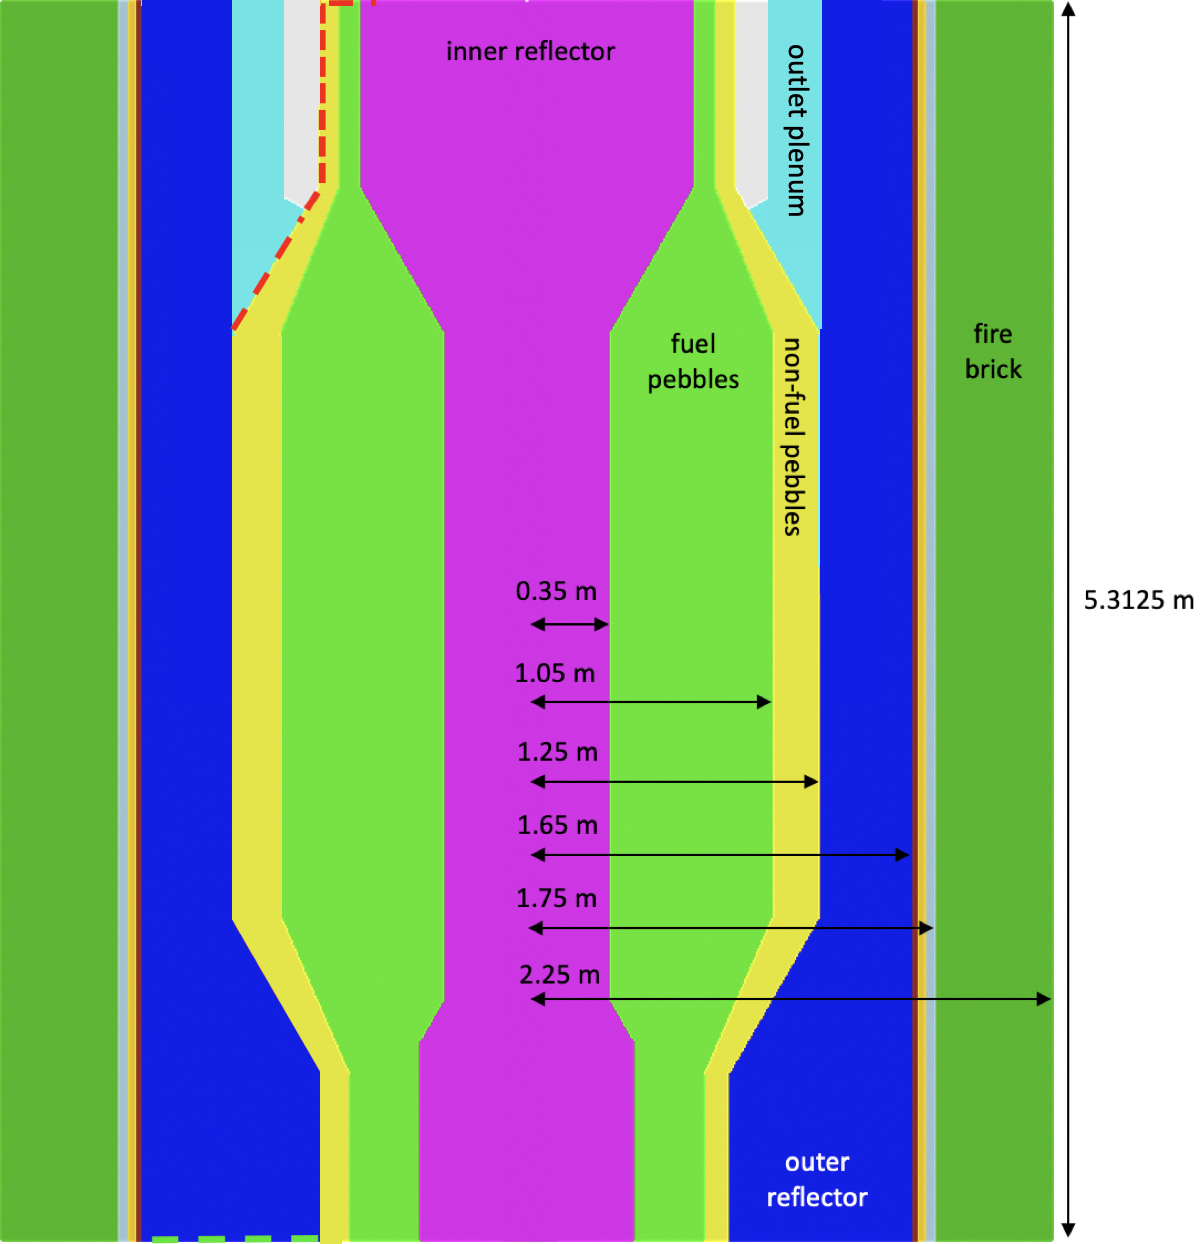
\includegraphics[width=0.5\linewidth]{figs/pbfhr_slice.png}
\caption{Slice through center of $r$-$z$ axisymmetric Pronghorn model of the \gls{pbfhr}.}
\label{fig:pbfhr_slice}
\end{figure}

A top-down schematic of a section of the outer reflector block model at the axial mid-plane of the reactor is shown in Fig.\ \ref{fig:orh}. Several simplifications have been made relative to the as-designed component shown in Fig.\ \ref{fig:pbfhr_ring}. The protruding ribs from the barrel and ``lips'' forming small sheaths between adjacent rings are neglected. While not shown in Fig.\ \ref{fig:pbfhr_ring}, the \gls{pbfhr} design report also describes triangular notches machined into the corners of each block with carbon fiber tube inserts to suppress vertical bypass flows; a lack of any visual depiction of these notches and tubings precludes their inclusion in the present work. 

\begin{figure}[h!]
\centering
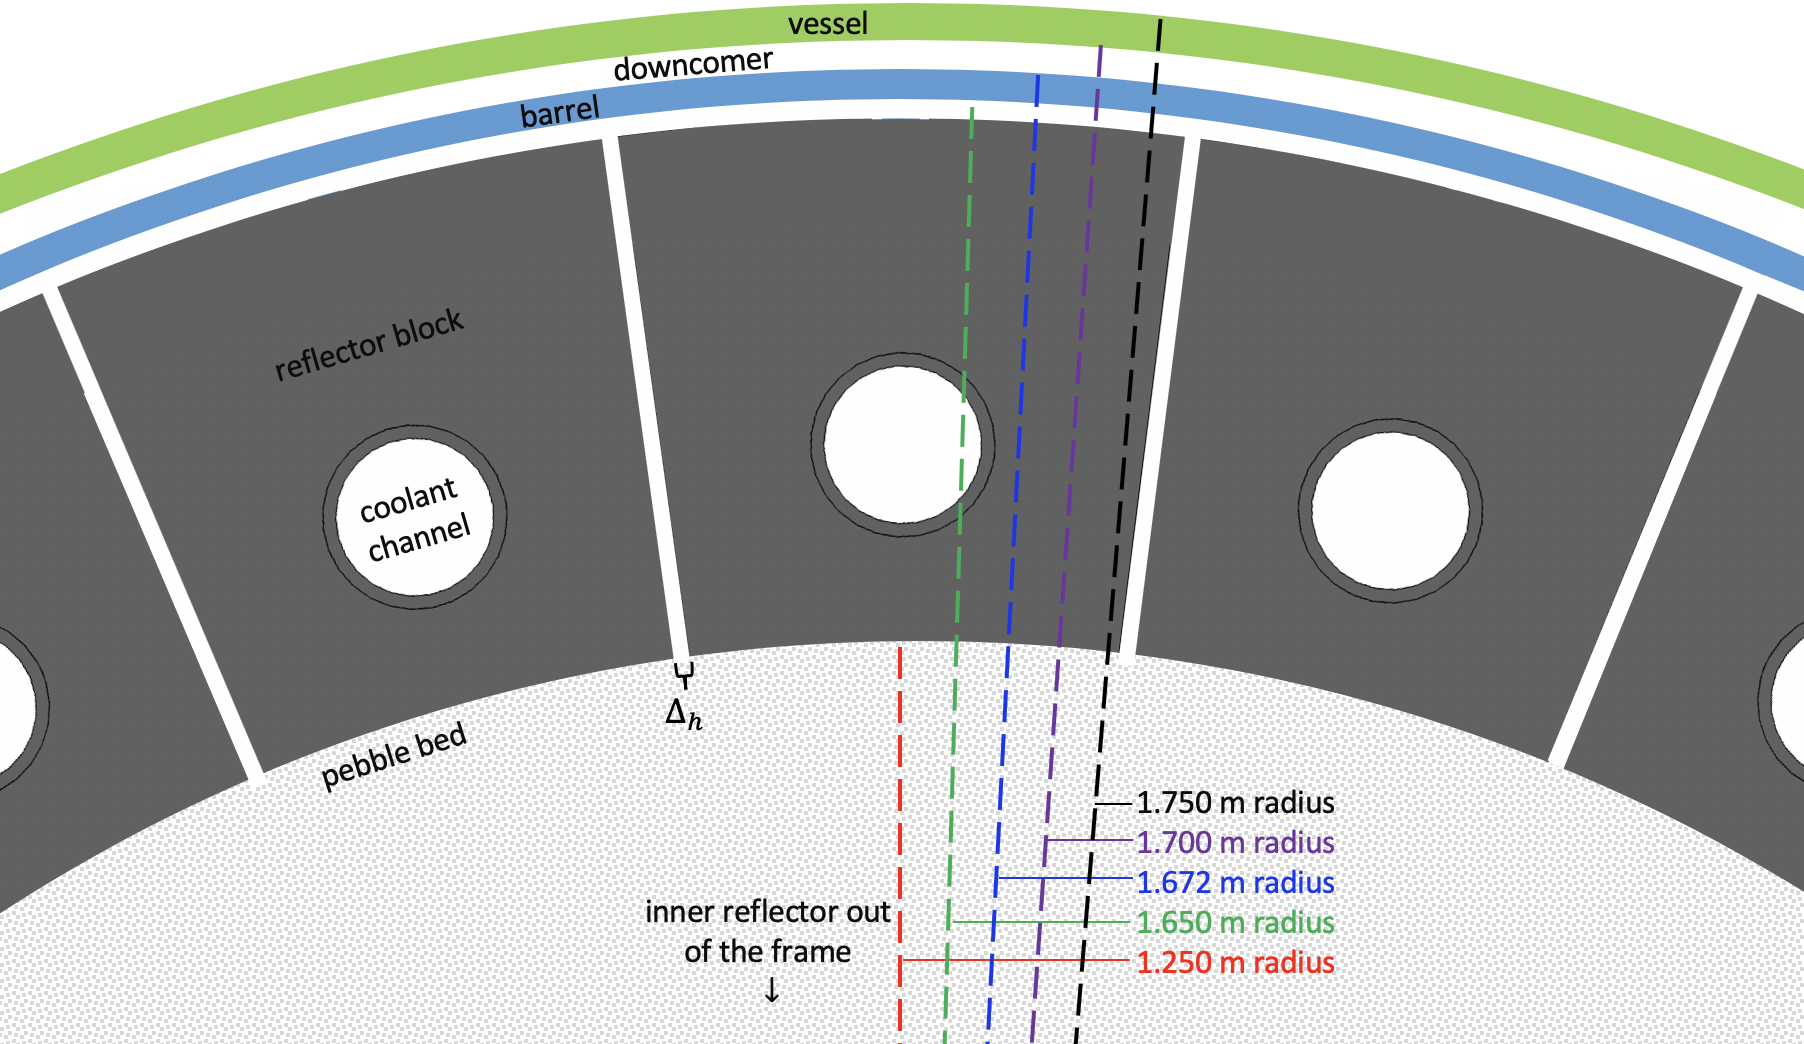
\includegraphics[width=0.8\linewidth]{figs/pbfhr_or.png}
\caption{Top-down schematic of a section of the outer reflector at the axial mid-plane of the \gls{pbfhr} as represented in COMSOL.}
\label{fig:orh}
\end{figure}

Gaps exist between the reflector blocks and between the barrel. The width of these gaps is represented as \(\Delta_h\) in Fig.\ \ref{fig:orh}. Gaps may also exist between each layer of blocks and the layers above and below due to as-manufactured contact gap tolerances and spatially-varying deformation. The width of these gaps between block rings is represented as \(\Delta_v\). Both the horizontal and vertical gaps are assumed to be uniform, which neglects the spatial dependence of the graphite dimensional changes and implies that the reflector blocks float relative to neighboring blocks above and below. The implications of this assumption are revisited in Section \ref{sec:conclusions_fhr}.

Finally, and perhaps most significantly, no geometric information is available for the reflector block design at axial positions away from the core mid-plane. For instance, the outer reflector thickness towards the bottom of the reactor is 0.793 \si{\meter}. Rather than arbitrarily assume the horizontal suction channels are 0.393 \si{\meter} longer than the design at the mid-plane or that no suction channels exist, requiring significantly more \gls{cfd} simulations, the entire outer reflector is modeled with the same closures as those calculated for the mid-plane blocks. Fig.\ \ref{fig:ord} shows more detailed schematics of the dimensions of a single outer reflector block at the axial mid-plane of the reactor with \(\Delta_h=0\) and \(\Delta_v=0\). 

\begin{figure}[h!]
    \begin{subfigure}{0.5\linewidth}
        \centering
        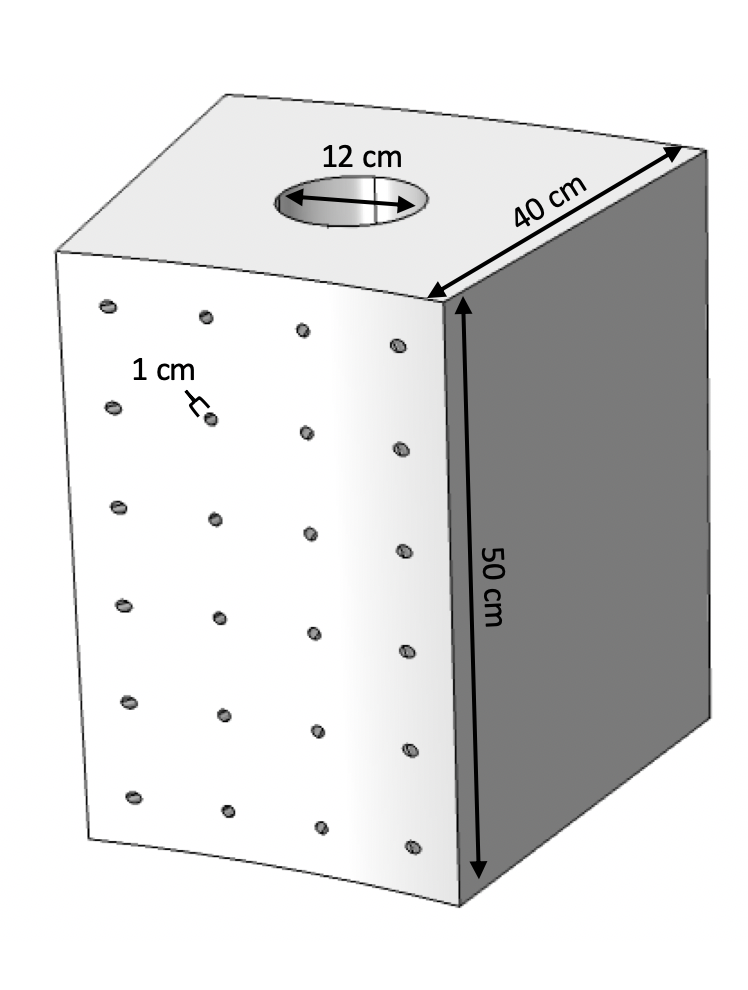
\includegraphics[width=0.6\linewidth]{figs/pbfhr_or2.png}
       \caption{Volume rendering}
    \end{subfigure}
    \begin{subfigure}{0.5\linewidth}
        \centering
        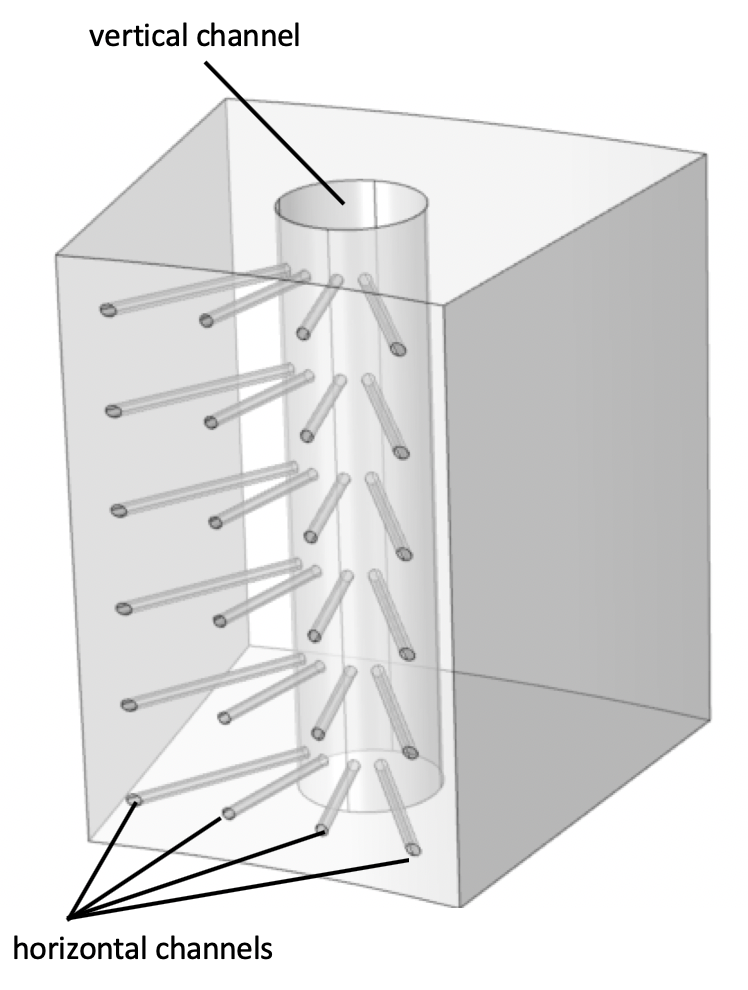
\includegraphics[width=0.6\linewidth]{figs/pbfhr_or1.png}
        \caption{Wireframe rendering}
    \end{subfigure}
    \caption{Schematic of the \gls{pbfhr} outer reflector blocks at the axial mid-plane as represented in COMSOL for \(\Delta_h=0\) and \(\Delta_v=0\) as (a) volumes and (b) wireframes.}
    \label{fig:ord}
\end{figure}

The pebble bed, outer reflector, and outlet plenum are modeled as porous media, while the barrel, vessel, and firebricks are modeled as conducting slabs. Small convective flows in gaps between the fire bricks are neglected. While coolant flows in the downcomer and inner reflector, both of these regions are also modeled as conducting slabs for two reasons. First, the inlet plenum geometry remains to be developed, so the geometry connecting the downcomer to the bed and reflectors is unknown. Second, the axial distribution of flow from the inner reflector into the bed is an open design question for the \gls{pbfhr} \cite{pbfhr,xin_wang_thesis,scarlat}. 

If the inner reflector were modeled as a porous medium, the interphase friction factor \(W\) as a function of height must be imposed in a manner to obtain the desired axial flow distribution, resulting in a complex nonlinear problem for every potential inlet flow \gls{bc}. Instead, the flow into the core is imposed on the inlet to the pebble bed region and along the inner reflector outer surface according to the desired axial distribution. The inner reflector is modeled as a two-phase conducting slab mixture of 50\% \gls{flibe} and 50\% graphite.

Many methods have been developed to model reflector bypass flows in \glspl{pbr}, with the particular geometry usually playing a role in model selection. The three most common approaches are to 1)~resolve a portion of the bypass paths and pebble bed, where a turbulence model is applied to the bypass regions and a porous media model to the bed region \cite{ximing,rensburg}; 2)~calculate reflector block resistance factors with off-line \gls{cfd} simulations that are used in a flow network model \cite{jun2011, liu_2018,wyk}; or 3)~model the reflector blocks as porous media.

The porous media approach is selected in the present study because of the more complex reflector structure in the \gls{pbfhr} than in the \gls{htrpm} and \gls{pbmr} designs that are the focus of the previously-cited works. While Pronghorn includes capabilities for modeling 1-D flow channels in a 3-D solid \cite{nrc_2020}, the presence of the 24 horizontal coolant channels precludes a clean separation of the vertical and horizontal flows. Further, the present analysis considers vertical gaps between blocks that may form due to spatially-varying irradiation- and temperature-induced deformation. 

In the porous regions, the friction-dominated macroscale model in Eqs. \eqref{eq:PMass2}--\eqref{eq:PSEnergy2} is used because of the relatively low Reynolds numbers expected. For the pebble bed region, \(\epsilon=0.4\) and \(W\), \(\alpha\), and \(\kappa_f\) are given by the Ergun model in Eq. \eqref{eq:Ergun}, the Wakao model in Eq. \eqref{eq:Wakao}, and the linear Peclet model in \eqref{eq:LinearPecletKappaFluid}, respectively. \(\kappa_s\) considers the combined heat transfer paths by radiation, conduction, and contact, and is given as the sum of Eqs. \eqref{eq:KappaRadiationBB}, \eqref{eq:KappaFluidConductionZS}, and \eqref{eq:KappaSolidConductionCT}. 

While outlet plena in \glspl{pbr} are frequently modeled as porous media \cite{ximing}, the lack of any geometric description of the \gls{pbfhr} outlet plenum requires simplified closure selection for this region. For the outlet plenum, \(\epsilon=0.5\); \(\kappa_f\) is given by the zero-dispersion model in Eq. \eqref{eq:KappaFluidBasic}; \(\kappa_s\) is given by volume average in Eq. \eqref{eq:VolumeAverageKappaSolid}; and \(\alpha=0\). The drag is approximated with the Churchill friction correlation assuming the outlet plenum consists of \(n_\text{pipe}\) 1 \si{\centi\meter} diameter pipes, where \(n_\text{pipe}\) is calculated based on the assumed 50\% porosity \cite{churchill}. Section \ref{sec:bypass} describes the generation of anisotropic drag models for the outer reflector with COMSOL \gls{cfd} simulations and Table \ref{table:porosity} provides the outer reflector porosity as a function of the block gap size. 

A total inlet flow of 976 \si{\kilo\gram\per\second} at 600\si{\celsius} is imposed along the inner reflector outer surface, the bottom of the pebble bed, and the bottom of the outer reflector. Beginning with zero bypass, the mass flowrate into the outer reflector is incrementally increased until the pressure at the bed and outer reflector inlet matches to within 10 \si{\pascal}, approximating the effect of an inlet plenum. An outlet pressure of 2 atm is imposed on all outflow boundaries. Due to the low flows expected, the fluid phase is assumed insulated on all walls. The solid phase is assumed insulated on all boundaries except the fire brick surface, where a temperature of 30\si{\celsius} is imposed to match the nominal operating temperature of the \gls{rrcls}. 

Fig.\ \ref{fig:high_level} summarizes the multiscale model and its application to the \gls{pbfhr}. The 2-D $r$-$z$ mesh, before applying a variety of surface and curve mesh refinements, is shown in the center. White arrows represent the flow \glspl{bc} into the core through the inner reflector, outer reflector, and pebble bed and out of the core through the pebble bed, outlet plenum, and outer reflector. The length of each arrow approximates spatially-nonuniform velocities.

\begin{figure}[h!]
\centering
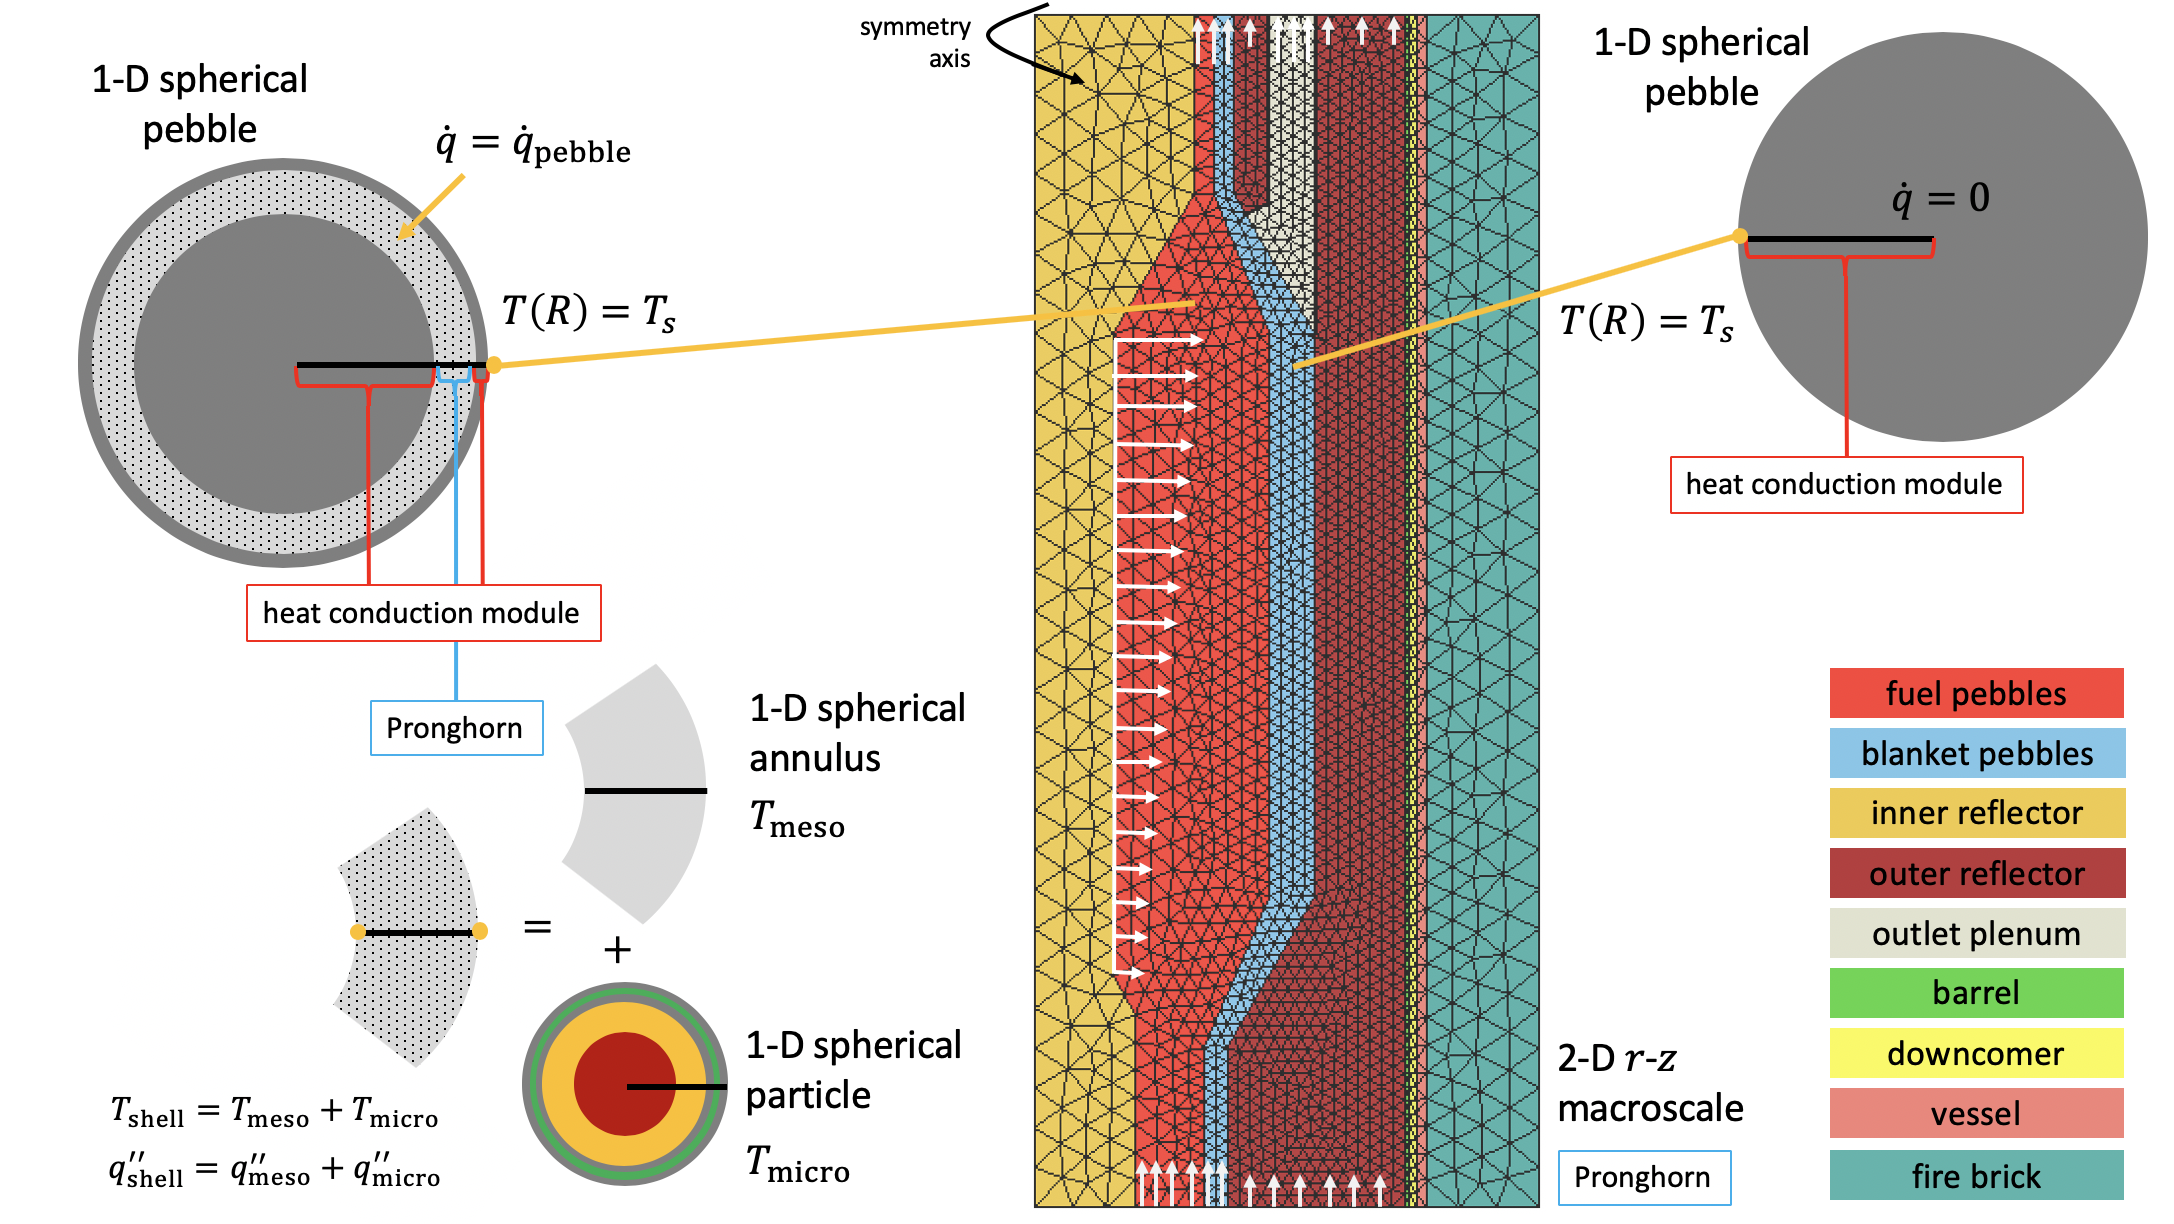
\includegraphics[width=\linewidth]{figs/high_level_pbfhr.png}
\caption{High-level summary of the multiscale method applied to the \gls{pbfhr}.}
\label{fig:high_level}
\end{figure}

Within each computational element of the macroscale mesh in the pebble region, the average power density and surface temperature are passed to a mesoscale model of a representative pebble as a source term and uniform Dirichlet \gls{bc}, respectively. For the fuel pebbles, the homogeneous graphite shell and core are modeled with the heat conduction equation, while the fuel-matrix annulus is modeled with the \gls{hsd} method. For the blanket pebbles, the absence of heterogeneous regions allows modeling directly with the heat conduction equation. Text boxes in Fig.\ \ref{fig:high_level} with ``heat conduction module'' and ``Pronghorn'' indicate that kernel objects from the \gls{moose} heat conduction module and the Pronghorn application, respectively, are used to construct the residual in those regions.

To enable reproduction of the simulations presented in this chapter, Appendix \ref{sec:reproducibility} lists all data and input files related to this chapter.

\section{Verification of the Meso and Micro Scale Models}
\label{sec:meso_fhr}

This section compares the \gls{hsd} and \gls{hl} methods against reference temperature solutions obtained with the \gls{moose} heat conduction module. The reference solutions are obtained on meshes that explicitly account for all \glspl{cfp} and their layers; these are referred to as ``fully-resolved'' pebbles. The objective is to assess the applicability of the \gls{hsd} and \gls{hl} meso and micro scale models to the \gls{pbfhr} design and quantify the error as a function of thermal and geometric conditions.

When applying the multiscale model described in Section \ref{sec:mesomicro} to the full core, the uniform surface temperature of a representative pebble in each element is obtained as the cell averaged value of the macroscale solid surface temperature. Therefore, the present investigation assumes a uniform pebble surface temperature \gls{bc} to decouple the pebble temperature solution from the macroscale model. This surface \gls{bc} is arbitrarily set to 1000\si{\celsius}, though the use of constant pebble properties simply shifts all temperatures downward by \(\delta_s\) if the surface \gls{bc} is instead \(1000-\delta_s\) \si{\celsius}.

The simulations performed here match the geometry and materials of the \gls{pbfhr} fuel pebble shown in Fig.\ \ref{fig:pbfhr_fuel} in all regards except that the particle \gls{pf} is varied from \(5\) to \(30.9\)\% to investigate applicability of the \gls{hsd} and \gls{hl} methods to variations in pebble design. The pebble power is held fixed at 236 MWth divided by the 470,000 fuel pebbles. A total of 11 reference pebbles are constructed at \glspl{pf} of 5.0, 7.5, 10.0, 12.5, 15.0, 17.5, 20.0, 22.5, 25.0, 27.5, and 30.9\%. The reference meshes are constructed with particle coordinates obtained using the random packing algorithms in the OpenMC Monte Carlo code with all \gls{cfp} layers resolved \cite{jodrey}. Only one sixteenth of the pebble is meshed to reduce runtime; any particles that are ``cut'' by the \(x=0\), \(y=x\), or \(z=0\) faces of the partial pebble are first removed. To preserve the correct \gls{pf}, those particles are each re-sampled with new random coordinates such that they are fully contained within the fuel-matrix annulus or their centers are on the cut faces. This permits insulated \glspl{bc} to be applied on all faces without geometric distortion. Simulations with full and eighth pebbles show negligible impact of this resampling on average and maximum material-wise temperatures, so the use of a sixteenth of a pebble is a reasonable model for the present analysis. 

Approximately \(2\times10^8\ p\) tetrahedral elements are used in the reference meshes, where \(p\) is the \gls{pf}. That is, the one-sixteenth reference pebble at 30.9\% \gls{pf} contains approximately \(60\times10^6\) elements. The \gls{hsd} and \gls{hl} methods each represent approximately five orders of magnitude reduction in the number of elements relative to the reference because the \gls{hsd} and \gls{hl} methods are run on a 1-D mesh.

Fig.\ \ref{fig:pebble_octant_mesh} shows a close-up view of a portion of the tetrahedral reference mesh at 20\% \gls{pf}. The colors represent the different materials present; the gray, purple, and red colors correspond to the graphite core, graphite matrix, and graphite shell, while the other colors represent the layers of the \gls{cfp}. Some elements may appear non-tetrahedral because of the particular manner in which the slice was taken in the mesh.

\begin{figure}[h!]
\centering
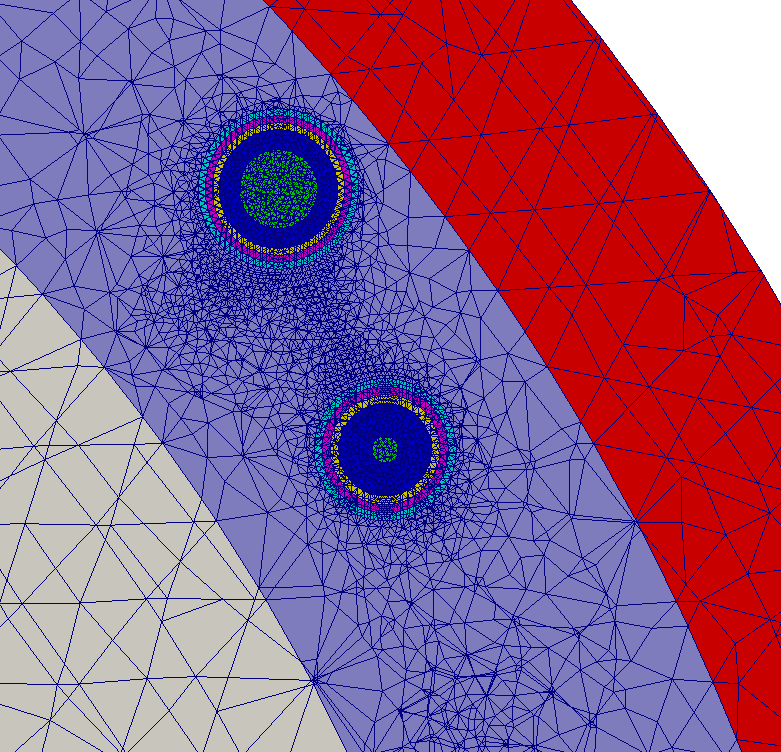
\includegraphics[width=0.4\linewidth]{figs/pbfhr_pebble_mesh_cross_section.png}
\caption{Close-up view of a portion of the tetrahedral reference mesh at 20\% \gls{pf}. The colors represent different materials present, with the gray, purple, and red colors corresponding to the graphite core, matrix, and shell, respectively; other colors represent the \gls{cfp} layers.}
\label{fig:pebble_octant_mesh}
\end{figure}

For illustration, Fig.\ \ref{fig:f1} shows the reference fuel kernel temperature solution for 15\% particle \gls{pf}. Temperatures in the matrix and all \gls{cfp} layers exterior to the central fissile kernel are not shown, while the core and shell regions are shown as gray blocks for scale. An inset shows the tetrahedral mesh in the \glspl{cfp}, where the color represents the material ID. Because the heat source is uniform and localized to the kernel, kernel temperatures are highest in the particle center.

\begin{figure}[h!]
\centering
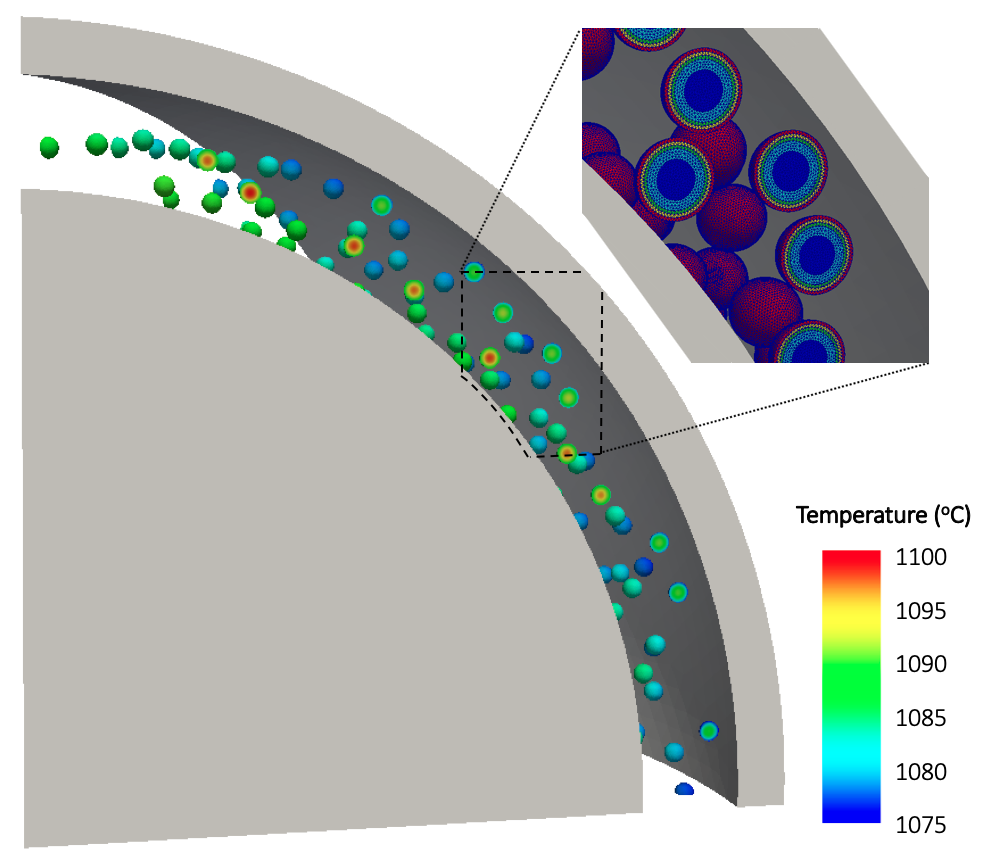
\includegraphics[width=0.5\linewidth]{figs/fhr_fuel1.png}
\caption{Reference temperature solution in the kernels for 15\% \gls{pf} with the shell and core shown as gray blocks.}
\label{fig:f1}
\end{figure}

To provide a second perspective at a different \gls{pf}, the reference temperature solution at \(20\)\% \gls{pf} is shown in Fig.\ \ref{fig:octant1} along a radial plane and in Fig.\ \ref{fig:octant2} on the surfaces of the particles with the core and shell shown for context. Different color scales are used to make results clearer. The absence of a heat source in the central graphite core results in a nearly uniform temperature distribution in this region, and the majority of the radial temperature drop occurs over the fuel-matrix region. Ten other simulations at different \glspl{pf} were performed, but for brevity not shown here.

\begin{figure}[!htb]
\centering
\begin{subfigure}{.475\textwidth}
  \centering
  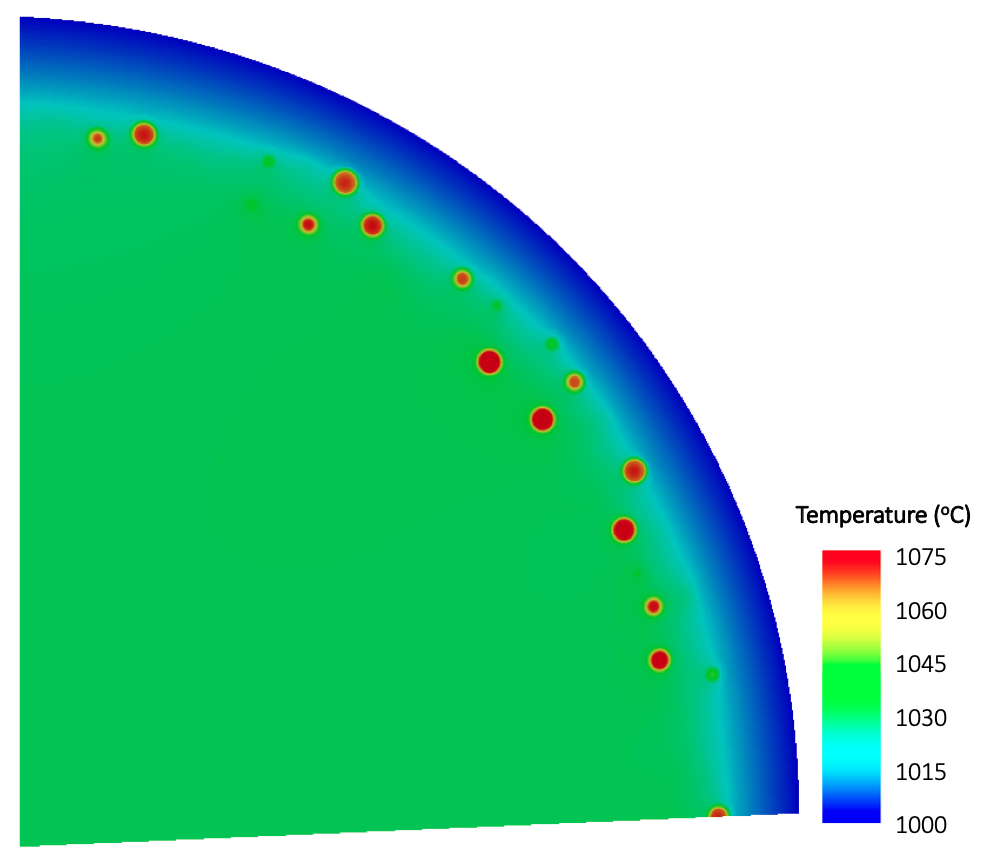
\includegraphics[width=\linewidth]{figs/fhr_fuel3.png}
  \caption{Along plane parallel to \(x\) axis}
  \label{fig:octant1}
\end{subfigure}
\begin{subfigure}{.475\textwidth}
  \centering
  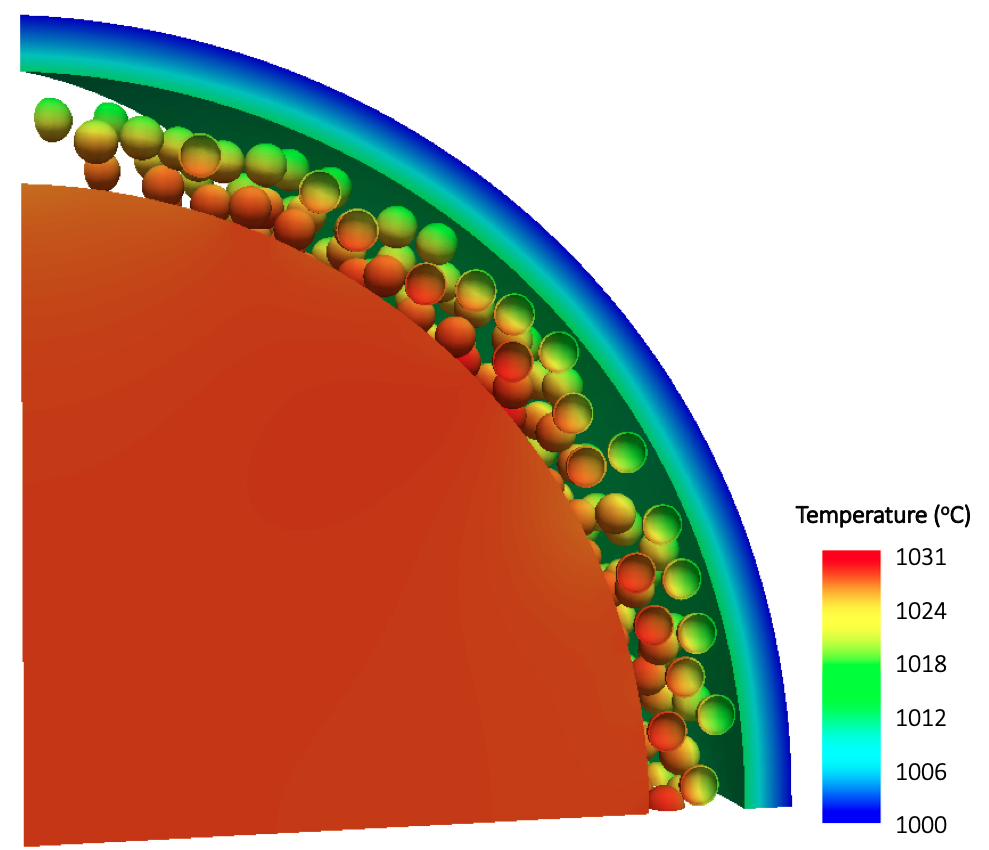
\includegraphics[width=\linewidth]{figs/fhr_fuel2.png}
  \caption{Particle surfaces with core and shell}
  \label{fig:octant2}
\end{subfigure}
\caption{Reference temperature solution for \(20\)\% \gls{pf} (a) along a radial plane and (b) on the surfaces of the particles, with the shell and core shown for context. Different temperature scales are used to enhance clarity.}
\label{fig:pebble_octant_ref}
\end{figure}

The \gls{hsd} method is applied with Eq. \eqref{eq:ChiewGlandt} used to average the fuel-matrix with the \glspl{cfp} and Eq. \eqref{eq:parallel} used for all other averages. After several trial-and-error tests, the \gls{hl} method is applied for two pseudo-particles; using a single particle resulted in poorer temperature predictions because of a reduced geometric attenuation, while no significant difference was observed for more than two pseudo-particles.

Figs. \ref{fig:hsd1} and \ref{fig:hsd2} compare the reference (dots), \gls{hsd} method (---), and \gls{hl} method \mbox{(- -)} integral temperature solutions as a function of \gls{pf}. The \gls{pf} corresponding to the \gls{pbfhr} fuel design is highlighted with a gray vertical line. The maximum kernel, average kernel, and average buffer temperatures are shown in Fig.\ \ref{fig:hsd1}, while average graphite temperatures in the core, matrix, and shell of the pebble are shown in Fig.\ \ref{fig:hsd2}. Different temperature scales are used to make results clearer.

\begin{figure}[!htb]
\centering
\begin{subfigure}{.49\textwidth}
  \centering
  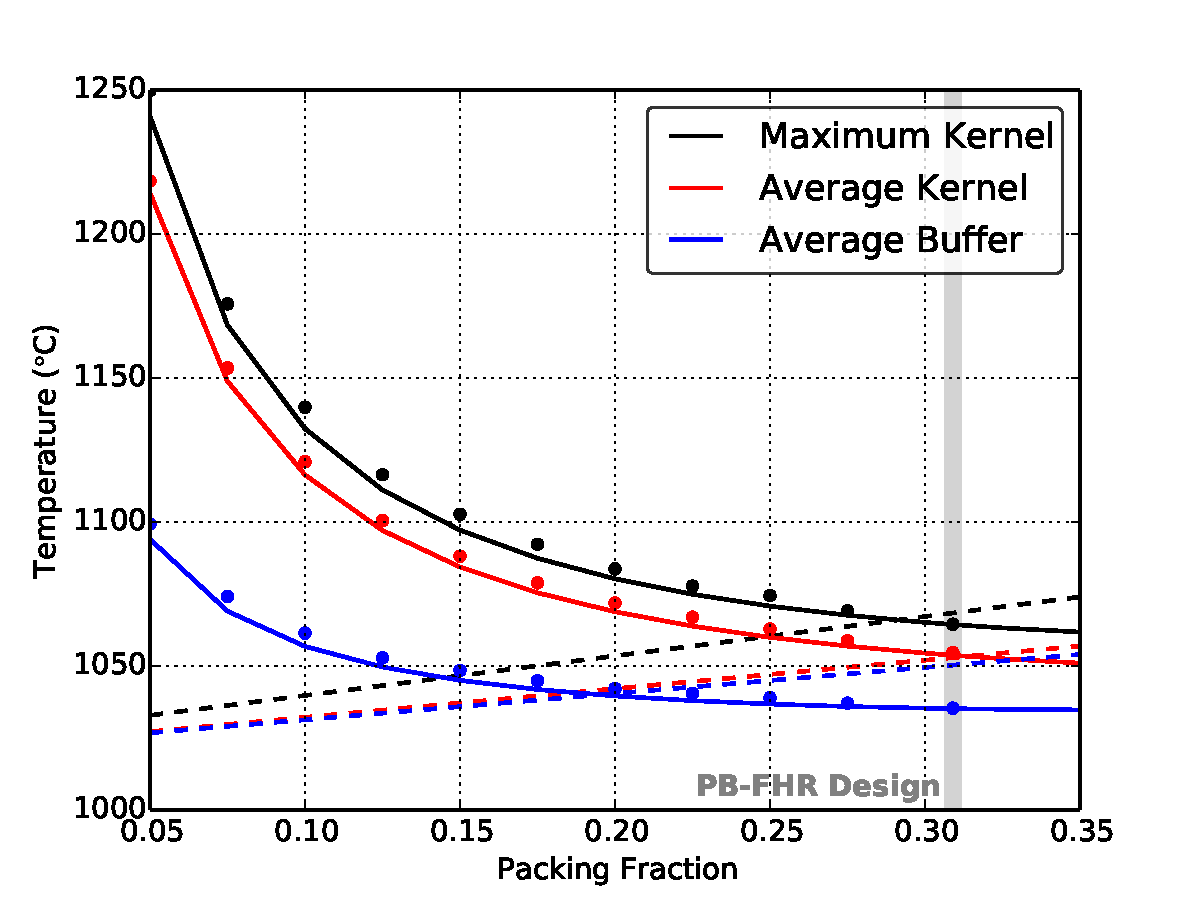
\includegraphics[width=\linewidth]{figs/hsd_hlm_0.pdf}
  \caption{Materials in particle}
  \label{fig:hsd1}
\end{subfigure}
\begin{subfigure}{.49\textwidth}
  \centering
  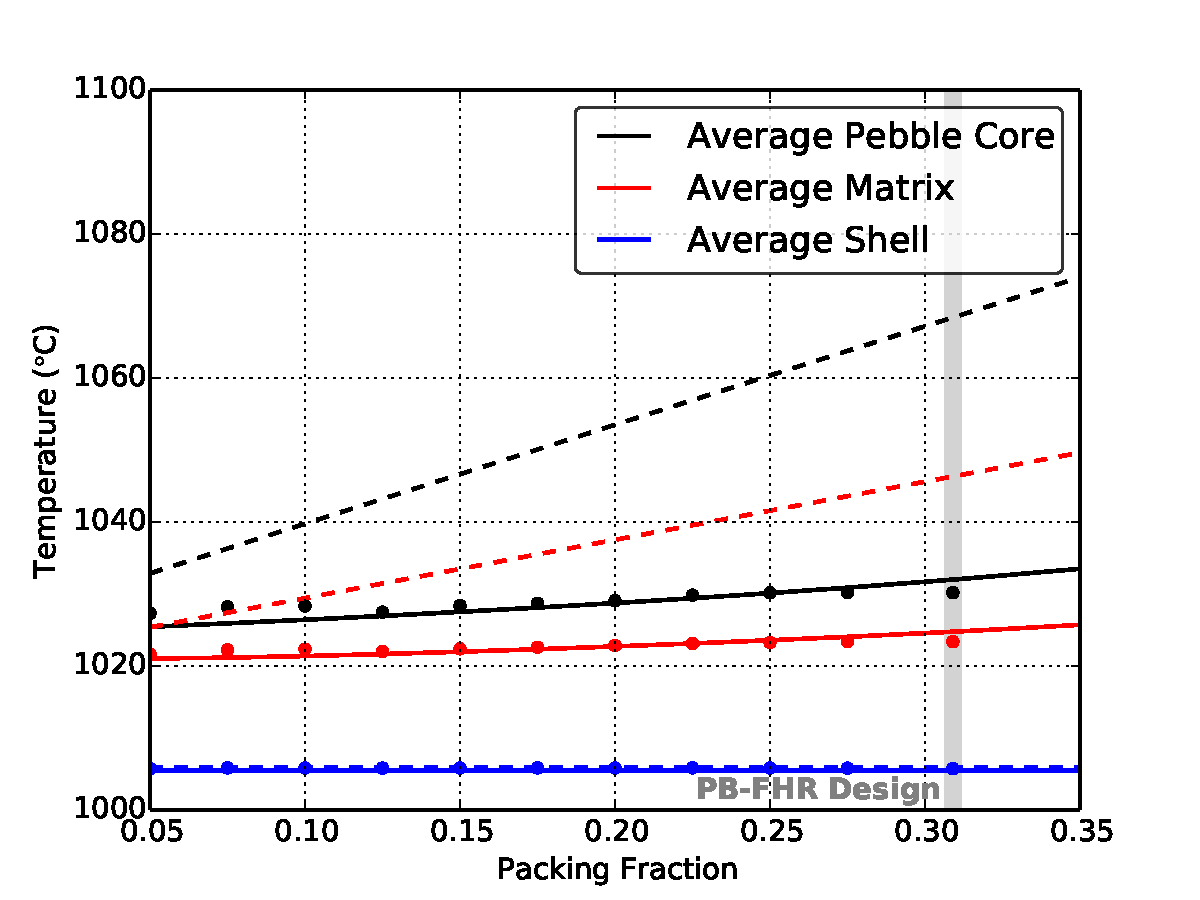
\includegraphics[width=\linewidth]{figs/hsd_hlm_1.pdf}
  \caption{Materials not in particle}
  \label{fig:hsd2}
\end{subfigure}
\caption{Reference ($\bullet$), \gls{hsd} (---), and \gls{hl} method (- -) integral temperature solutions for (a) materials within the particle and (b) materials not within the particle as a function of \gls{pf}.}
\label{fig:hsd_hlm}
\end{figure}

As shown in Fig.\ \ref{fig:hsd1}, the temperature in each layer of the particle decreases with increasing \gls{pf} because the power per particle decreases. As shown in Fig.\ \ref{fig:hsd2}, the temperature in regions outside the particle increases slightly with \gls{pf} because the effective thermal conductivity of the heterogeneous region decreases with the replacement of relatively high thermal conductivity matrix by lower thermal conductivity \glspl{cfp}.

The \gls{hsd} is in remarkably good agreement with the reference solution over all ranges in \gls{pf}. The maximum error over all \glspl{pf} for regions within the particle is only 9.0\si{\celsius}, and occurs for the maximum kernel temperature at the lowest \gls{pf} where clustering effects are the most significant. The maximum error for regions outside the particle is only 2.3\si{\celsius}. Conversely, the accuracy of the \gls{hl} method is strongly affected by \gls{pf}, since the \gls{pf} determines the overall thermal resistance from the pseudo-particles to the matrix. The smaller the \gls{pf}, the thinner the layers surrounding the pseudo-particles and the smaller the overall resistance. The total thermal resistance increases with \gls{pf}; therefore, the \gls{hl} method predicts increasing temperatures within all particle layers with increasing \gls{pf} due to the continual increase in resistance, a nonphysical trend. The \gls{hl} method predicts nearly identical average kernel and buffer temperatures, which demonstrates a general failure to capture the thermal resistance.

While the \gls{hl} method predicts the correct trend of increasing temperatures outside the particle with \gls{pf} in Fig.\ \ref{fig:hsd2}, the error increases with \gls{pf}. This occurs because of a combination of lower effective thermal conductivity and the division of the continuous matrix material into increasingly separated segments. The \gls{hl} method does not converge to the reference at either low or high \gls{pf}, and nonphysical particle temperature trends with \gls{pf} do not establish confidence in the robustness of the method. 

Because a single reference solution is obtained at each \gls{pf}, the variations of the temperature distribution originating from the stochastic nature of the particle distribution have been neglected. For a similar \gls{cfp} design, Liu et al.\ estimate a 5\si{\celsius} standard deviation in temperatures associated with the stochastic particle distribution \cite{liu}. Future work extending this dissertation will perform multiple reference calculations to estimate the standard deviation for the \gls{pbfhr} design.

Table \ref{table:error} summarizes the error in the \gls{hsd} and \gls{hl} solutions for the nominal \gls{pbfhr} design at 30.9\% \gls{pf}. The \gls{hsd} method predicts all temperatures to within 1.8\si{\celsius}, which supports the use of the \gls{hsd} method for steady-state analysis of the \gls{pbfhr}. It is rather fortuitous that a reasonable agreement is obtained for the \gls{hl} method for the maximum and average kernel temperatures given the general failure to predict temperatures over the \gls{pf} range investigated. The underprediction of the \gls{cfp} thermal resistance and the division of the continuous matrix results in temperature overpredictions of \(22.3\) to \(38.2\)\si{\celsius} in regions outside the kernel aside from the shell. The \gls{hl} method is not recommended for analysis of the \gls{pbfhr} because of its inability to account for thermal resistance in low-\gls{pf} fuel variations, and hence is not considered further in this chapter.

\begin{table}[htb!]
\caption{Temperature error (multiscale minus reference) for the \gls{hsd} and \gls{hl} methods applied to the nominal \gls{pbfhr} fuel design at 30.9\% \gls{pf}.}
\centering
\small
\centerline{
\begin{tabular}{|r| c c c|c c c|}
\hline\hline
\multirow{2}{*}{}& Maximum & Average & Average & Average & Average & Average\Tstrut\\
& Kernel & Kernel & Buffer & Matrix & Pebble Core & Pebble Shell\Bstrut\\
\hline
HSD Error (\si{\celsius}) & $-0.1$ & $-0.9$ & $\color{white}0\color{black}-0.2$\hspace{0.15cm} & $\color{white}0\color{black}1.4$ & $\color{white}0\color{black}1.8$ & $-0.2$\Tstrut\\
HL Error (\si{\celsius}) & $\color{white}-\color{black}3.9$ & $-1.7$ & $\color{white}-\color{black}22.3$ & $22.9$ & $38.2$ & $\color{white}-\color{black}0.1$\Bstrut\\
\hline
\end{tabular}
}
\label{table:error}
\end{table}

The uniquely ``thermally-thin'' fuel-matrix region may explain the high accuracy of the \gls{hsd} and the low accuracy of the \gls{hl} method. Only at relatively high \glspl{pf} can the \gls{hl} method reasonably approximate the thermal resistance while preserving volume fractions with cubic spherical weighting. In addition, the approximations made in the effective mesoscale properties in the \gls{hsd} method are of smaller absolute consequence because of the thin shell thickness. 

To expand upon this last point, Fig.\ \ref{fig:hsd_err} shows the error (\gls{hsd} multiscale minus reference) as a function of \gls{pf} for integral temperature solutions (a) in the particle and (b) outside the particle for four different closure selections. Solid (---) lines correspond to the Chiew and Glandt model in Eq. \eqref{eq:ChiewGlandt} for the fuel-matrix with a parallel average for all other mixtures. Dashed (- -) lines correspond to the Chiew and Glandt model for the fuel-matrix with a series average for all other mixtures. Dashed-dot ($-\cdot-$) lines correspond to the Lewis and Nielsen model in Eq. \eqref{eq:Nielsen} for the fuel-matrix with a parallel average for all other mixtures. Dotted ($\cdots$) lines correspond to the Lewis and Nielsen model for the fuel-matrix with a series average for all other mixtures. In other words, two different fuel-matrix closures and two different \gls{cfp} and pebble layer closures are considered; the permutation gives four total sets of homogenization closures.

\begin{figure}[!htb]
\centering
\begin{subfigure}{.49\textwidth}
  \centering
  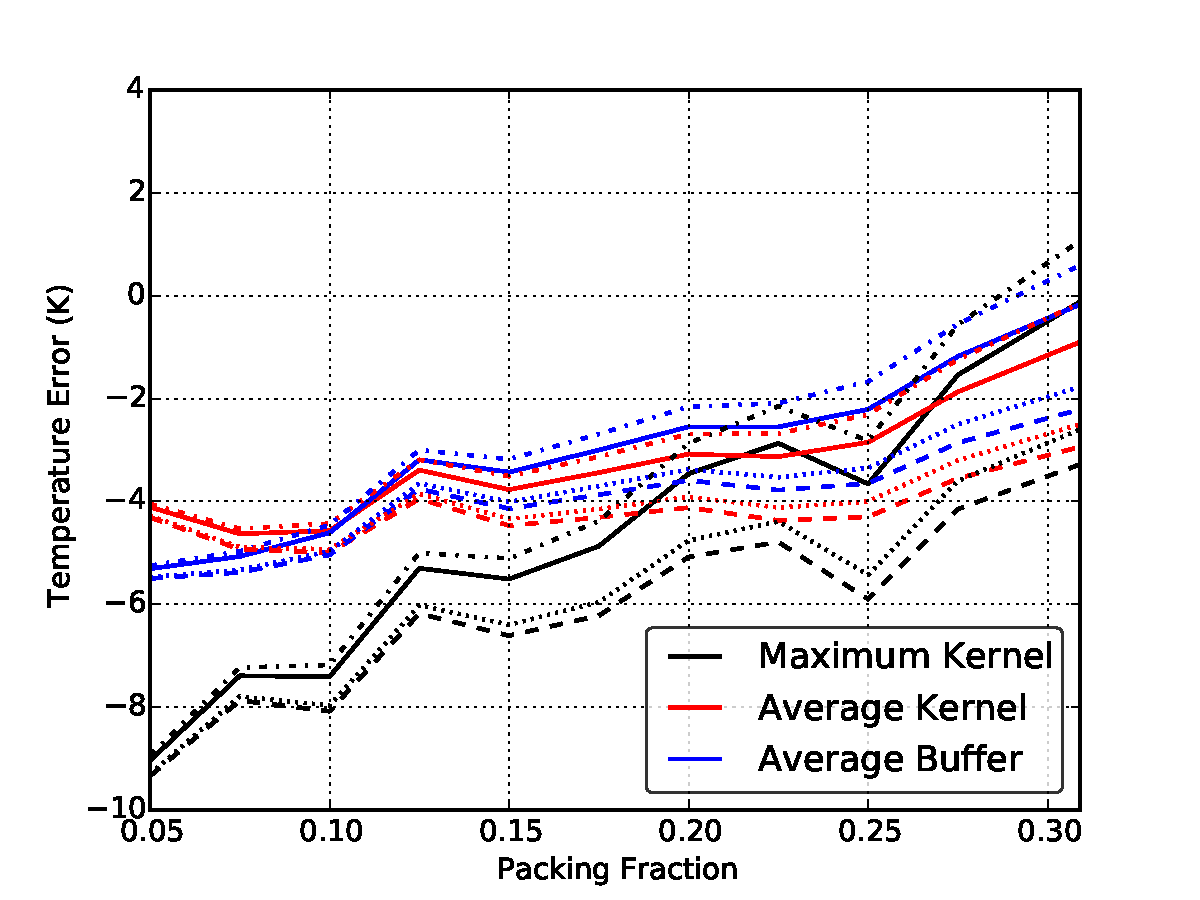
\includegraphics[width=\linewidth]{figs/hsd_error0.pdf}
  \caption{Materials in particle}
\end{subfigure}
\begin{subfigure}{.49\textwidth}
  \centering
  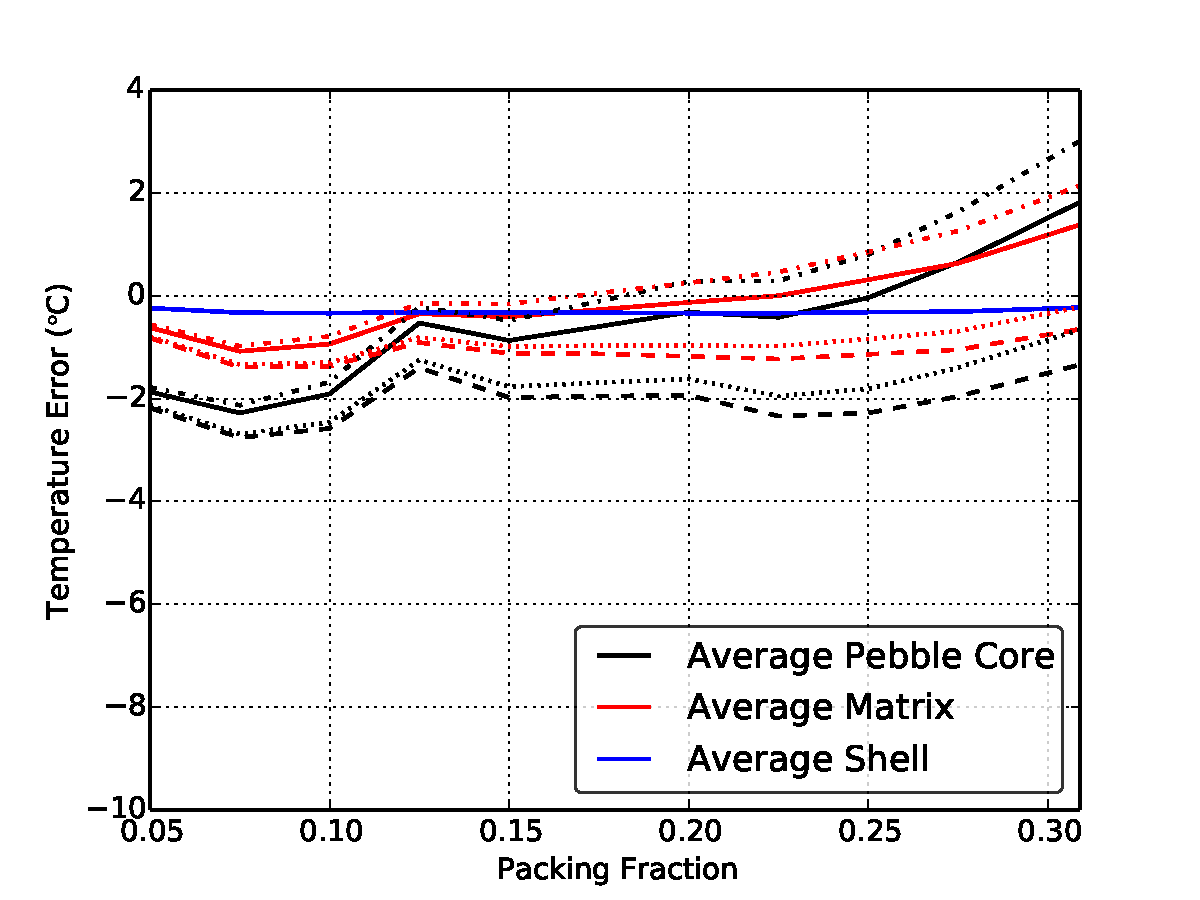
\includegraphics[width=\linewidth]{figs/hsd_error1.pdf}
  \caption{Materials not in particle}
\end{subfigure}
\caption{Integral temperature solutions for (a) materials within the particle and (b) materials not within the particle as a function of \gls{pf}. Solid (---) lines: Chiew and Glandt with parallel average; dashed (- -) lines: Chiew and Glandt with series average; dashed-dot ($-\cdot -$) lines: Lewis and Nielsen with parallel average; and dotted ($\cdots$) lines: Lewis and Nielsen with series average. }
\label{fig:hsd_err}
\end{figure}

The difference in temperature predictions among the various mixing closures generally increases with \gls{pf} as the fuel-matrix acts more as a mixture and less like pure graphite. However, the maximum difference in temperature predictions for all \gls{pf} is only about 4\si{\celsius}, demonstrating the relative insensitivity of the \gls{pbfhr} pebble temperature predictions to mixing closures for the thin fuel-matrix region. Jagged behavior in the error likely occurs due to small stochastic differences in the distance between the stochastic particle distribution and the mean distribution. In absolute terms, the non-smooth error behavior as a function of \gls{pf} is only on the order of 1\si{\celsius}. In general, temperatures are more sensitive to the series or parallel \gls{cfp} averaging model than to the binary Chiew and Glandt or Lewis and Nielsen mixing method for the fuel-matrix properties. 

It should be emphasized that the conclusions obtained in this section only apply to steady-state modeling of the \gls{pbfhr}. Similar verifications should be performed before application of the \gls{hsd} and \gls{hl} models to transients in the \gls{pbfhr} or to gas-cooled reactor fuel pebbles with thicker characteristic fuel-matrix regions.

\section[Computational Fluid Dynamics Modeling of Bypass Flows]{CFD Modeling of Bypass Flows}
\label{sec:bypass}

This section presents COMSOL \gls{cfd} modeling of flow through the \gls{pbfhr} outer reflector blocks; the objective is to obtain anisotropic drag correlations with form given by Eq. \eqref{eq:W3} to predict the maximum core bypass fraction. The presence of horizontal suction channels and a lack of graphite keys in the \gls{pbfhr} outer reflector block precludes the use of drag models developed for the \gls{htrpm} or \gls{pbmr}. After describing the \gls{cfd} model, correlation methodology, and mesh refinement study, anisotropic drag correlations are provided and select velocity and pressure predictions are shown.

Irradiation-induced dimensional changes in graphite are a complex function of the raw materials, manufacturing process, isotropy, in-service load conditions, and operating temperature \cite{marsden}. Generally, graphite initially shrinks and later swells during service. Temperature changes during transients and the resultant differential thermal expansion of the graphite and steel core structures also contribute to dimensional changes; for instance, the thermal expansion coefficient of steel may be five times that of graphite \cite{marsden}. Neutron flux and temperature gradients over the reflector blocks on core peripheries are usually large enough that dimensional changes may also be a function of position, especially in the 10 to 20 \si{\centi\meter} facing the bed \cite{oehme}.

Predicting the reflector block gap size with coupled solid mechanics and microstructure models is beyond the scope of the present investigation. Instead, the objective of this analysis is to predict the maximum core bypass fraction over the reflector lifetime, which represents the greatest diversion of coolant from the fuel. While core bypass has a significant effect on coolant and fuel temperatures, this effect has been assigned a medium-level importance in \glspl{pirt} because the maximum core bypass fraction can be bounded by assuming a limiting reflector gap size \cite{gou_2018}. For example, a maximum block shrinkage of 2\% was assumed for the \gls{thtr} \cite{oehme}.

The protective graphite pebble layer in the \gls{pbfhr} likely results in lower fluence in the outer reflector than in the non-shielded \gls{thtr}, so a maximum shrinkage of 1\% is assumed in this investigation. Assuming uniform and isotropic gaps, this shrinkage corresponds to gaps of 5 \si{\milli\meter} width, which is comparable to values suggested in other bypass flow studies \cite{liu_2018, viljoen,jun2011}. Further, to obtain a coarse understanding of the extent to which the gap size affects the core bypass fraction, a gap size of 10 \si{\milli\meter} is also considered. While a 10 \si{\milli\meter} gap size is likely unrealistically large when applied to the entire outer reflector, a gap size of 10 \si{\milli\meter} could be considered the maximum gap size in the areas of highest fluence.

Fig.\ \ref{fig:blocks} shows the two COMSOL representations of a \gls{pbfhr} outer reflector block for the 10 \si{\milli\meter} gap size\mdash Fig.\ \ref{fig:vertical} depicts the flow model used to correlate the drag in the axial direction and Fig.\ \ref{fig:horizontal} depicts the flow model used to correlate the drag in the horizontal direction. Symmetry permits modeling of half a block for the vertical flows and a quarter of a block for the horizontal flows, though this quarter-block geometry is not shown in Fig.\ \ref{fig:horizontal}. Inlet, outlet, and symmetry boundaries are indicated, with all remaining boundaries modeled as no-slip walls. A uniform velocity is imposed on inlet boundaries, while a uniform atmospheric pressure is imposed on outlet boundaries.

\begin{figure}[!htb]
\centering
\begin{subfigure}{.49\textwidth}
  \centering
  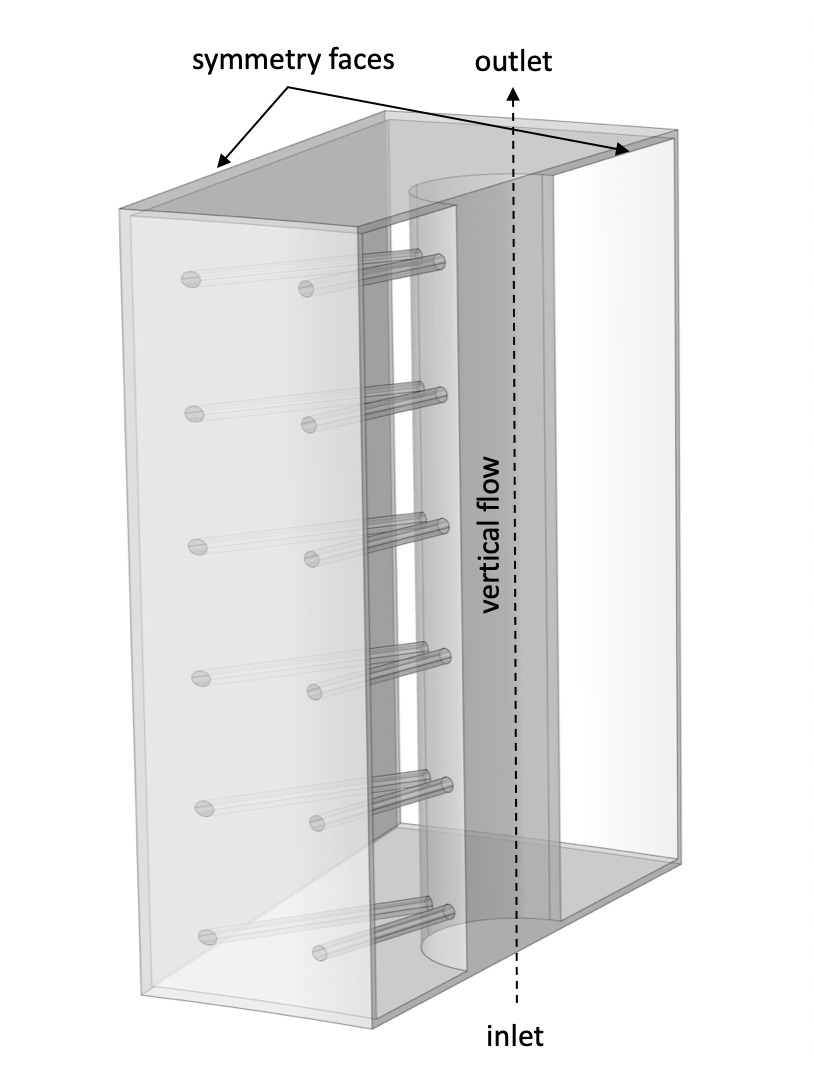
\includegraphics[width=0.85\linewidth]{figs/vertical.png}
  \caption{Vertical flow geometry}
  \label{fig:vertical}
\end{subfigure}
\begin{subfigure}{.49\textwidth}
  \centering
  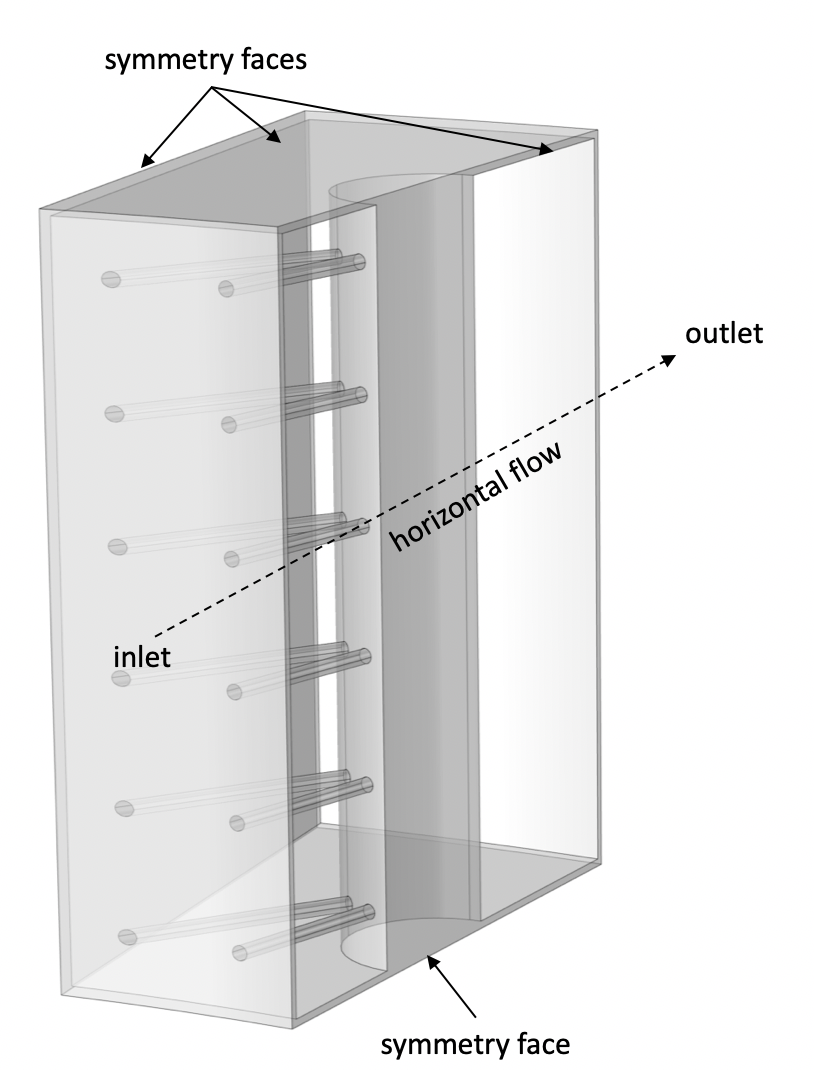
\includegraphics[width=0.85\linewidth]{figs/horizontal.png}
  \caption{Horizontal flow geometry}
  \label{fig:horizontal}
\end{subfigure}
\caption{(a) Vertical and (b) horizontal COMSOL models of the \gls{pbfhr} outer reflector block with inlet, outlet, and symmetry boundaries indicated. All other boundaries are no-slip.}
\label{fig:blocks}
\end{figure}

The complex geometry of the outer reflector block introduces several complications in the use of a porous media macroscale model for this region. In the reflector, the characteristic macro length scale \(L\) is on the same order as the characteristic meso length scale \(l\), and the averaging theorems in Appendix \ref{sec:PorousMediaMath} used to derive the porous media equations in Chapter \ref{sec:PhysicalModels} are less accurate when \(l/L\approx1\). Provided the macroscale model is understood to represent flow and heat transfer averaged over a group of blocks or even a group of quarter-blocks, the length scale criterion of \(l\ll L\) can more closely be satisfied.

Related to the smaller scale separation than in the pebble region, the porosity and hydraulic diameter in the reflector are both functions of position to a larger extent than in the bed. For simplicity of model correlation and based on the quarter-block averaging interpretation, both the porosity and hydraulic diameter are taken as uniform in space. Because of the different no-slip \glspl{bc} in the two cases shown in Fig.\ \ref{fig:blocks}, the hydraulic diameter is different for the vertical and horizontal models. Table \ref{table:porosity} provides the porosity and hydraulic diameters for the two gap sizes considered.

\begin{table}[htb!]
\caption{Outer reflector porosity and hydraulic diameter as a function of the gap size.}
\centering
\small
\begin{tabular}{|c| c c c|}
\hline\hline
Gap size (\si{\milli\meter}) & Porosity & Vertical \(D\) (\si{\centi\meter}) & Horizontal \(D\) (\si{\centi\meter})\\
\hline
\color{white}0\color{black}5.0 & 0.112 & 2.00 & 2.58\\
10.0 & 0.146 & 2.65 & 3.43\\
\hline
\end{tabular}
\label{table:porosity}
\end{table}

While two-equation turbulence models are usually employed for \gls{cfd} simulations of \gls{pbr} reflector blocks \cite{ximing,peng,wyk,liu_2018}, limited project resources restricted the present analysis to the incompressible Navier-Stokes equations with the Spalart-Allmaras turbulence model. The Spalart-Allmaras model is robust, fast, and often recommended as an \gls{ic} for complex two-equation industrial simulations. However, the model is known to be less accurate for shear flows and decaying turbulence, and may underpredict flow separation. 

Ideally, the \gls{cfd} simulations presented in this section would be compared against experimental data to guide turbulence model selection. For example, comparisons against experimental data revealed that Van Wyk's two-layer \gls{rng} \(k\)-\(\varepsilon\) simulations of a simplified \gls{pbmr} outer reflector block exhibited pressure drop errors on the order of 100 to 200\% \cite{wyk}. The complex block geometry of the \gls{pbfhr} makes a priori estimates of the error associated with the use of a one-equation turbulence model difficult. With an abundance of conservatism, errors as high as several hundred percent may exist in the friction factor predictions later in this section. However, the present simulations are still expected to capture the relative change in the friction factor as the block gap size is varied, an important objective in the consideration of multiple block gap widths. A sensitivity analysis will be performed in the future to propagate the uncertainty in the outer reflector friction factor correlation to the core bypass fraction.

\gls{flibe} properties are assumed constant and obtained from the correlations provided in Appendix \ref{sec:props} at 650\si{\celsius}, the nominal average bed fluid temperature \cite{novak_manual}. An automatic wall treatment switches between a low-Reynolds-number formulation and a wall function formulation depending on the mesh resolution near the wall. All other turbulence parameters in the Spalart-Allmaras model use default settings; for full details, the reader is referred to the COMSOL documentation \cite{comsol_cfd}.

Given the assumptions made in the block geometry and the use of the relatively coarse porous media model for the reflector region, a one-equation turbulence model is of comparable fidelity. Future work will repeat these calculations with more accurate turbulence models as more refined reflector geometry specifications become available.

Vertical and horizontal models are simulated for Reynolds numbers in the range of 250 to 2000. For the vertical flow direction, this upper limit is based on a maximum 30\% bypass into the reflector, or the complete diversion of the non-inner-reflector flow from the pebble bed to the outer reflector. For the horizontal flow direction, this upper limit is based on 100\% of the total mass flow passing horizontally through the reflector with a uniform axial distribution. Coincidentally, both of these limits are nearly the same and slightly below 2000, hence the selection of an upper Reynolds number of 2000.

For each flow direction, a mesh refinement study is performed for the highest Reynolds number of 2000. The bulk of the mesh consists of tetrahedral elements, with boundary layers meshed with prismatic elements and a stretching factor of 1.2. The mesh is progressively refined near the no-slip walls by halving the thickness of the first boundary layer cell and increasing the number of boundary layer cells by 50\% until the relative change in the friction factor is less than 5\%.

Fig.\ \ref{fig:velocity_5} shows COMSOL predictions of the velocity streamlines for a 5 \si{\milli\meter} gap at Reynolds numbers of (a) 500 and (b) 2000 in the two flow directions. For each Reynolds number, the velocities are shown on the same color scale, with the horizontal flow case shown on the left and the vertical flow case shown on the right. For horizontal flow, \gls{flibe} passes through the horizontal channels and expands within the vertical coolant channel, with several jets impinging on the back wall of the vertical channel. The fluid is then redirected downwards and flows to the back of the block through the thin gap between adjacent rings of blocks. For vertical flow, the incoming fluid is split between the vertical coolant channel and flow through the gaps on the front, back, and side of the block. A nearly circular ``stagnation'' line delineates these two flow paths. A small amount of the flow also passes through the horizontal flow channels between the vertical channel and the bed region.  

\begin{figure}[!htb]
\centering
\begin{subfigure}{\textwidth}
  \centering
  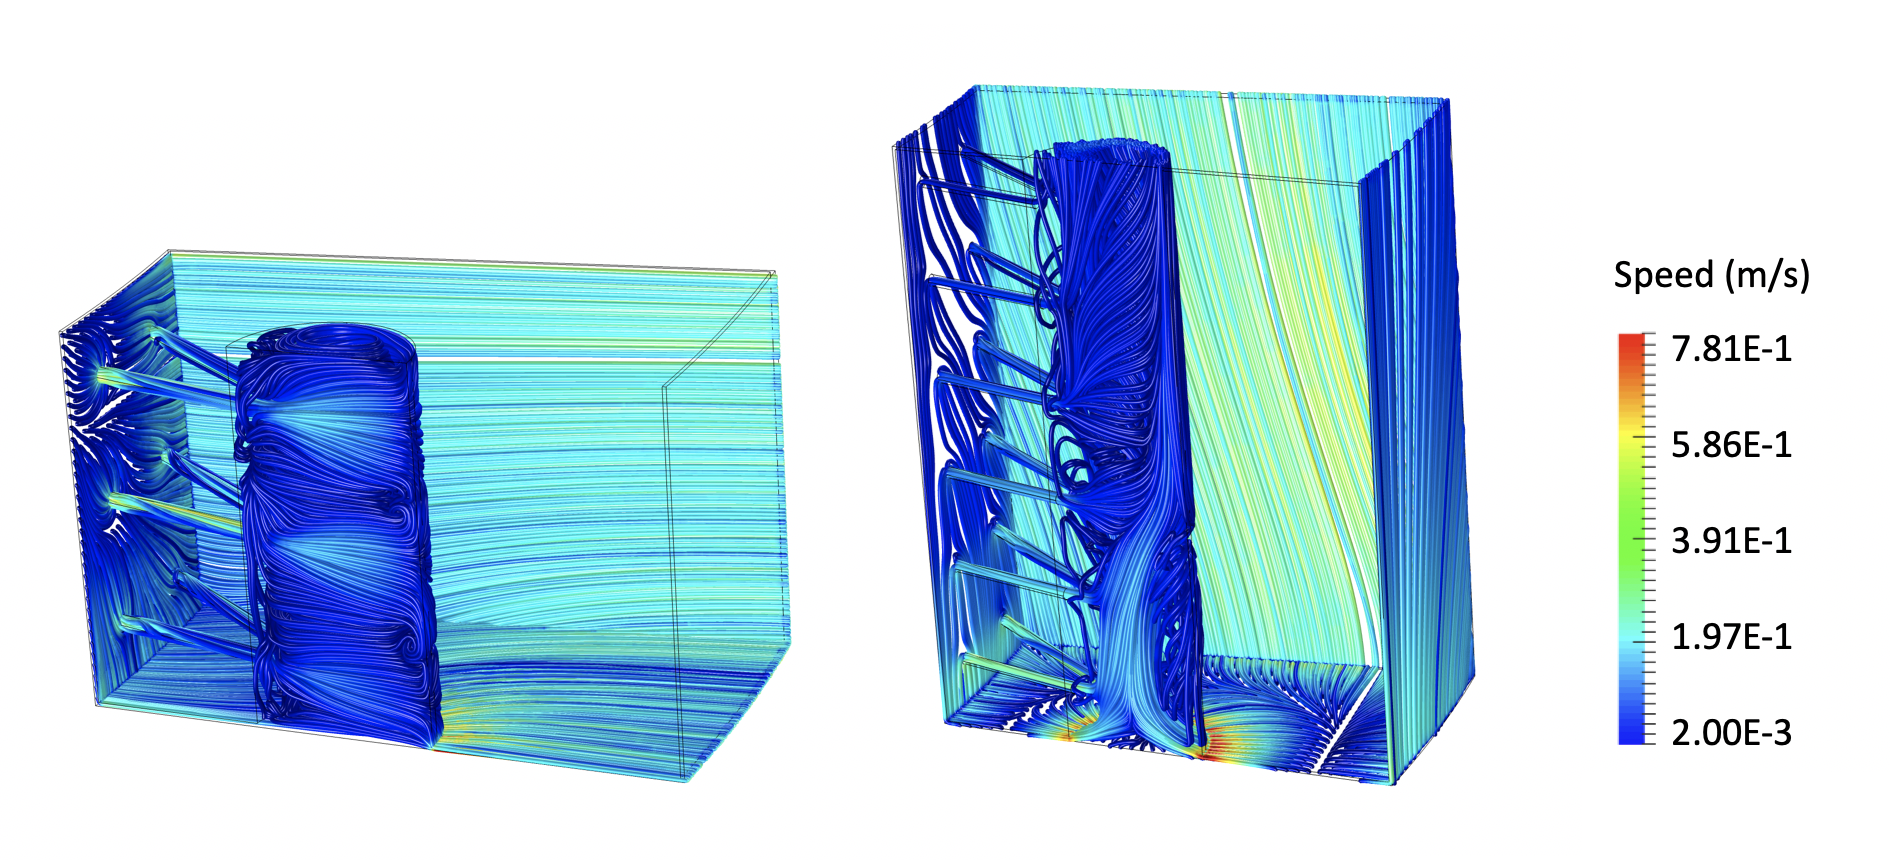
\includegraphics[width=0.8\linewidth]{figs/Re500_cm05_U.png}
  \caption{\(Re=500\)}
\end{subfigure}
\begin{subfigure}{\textwidth}
  \centering
  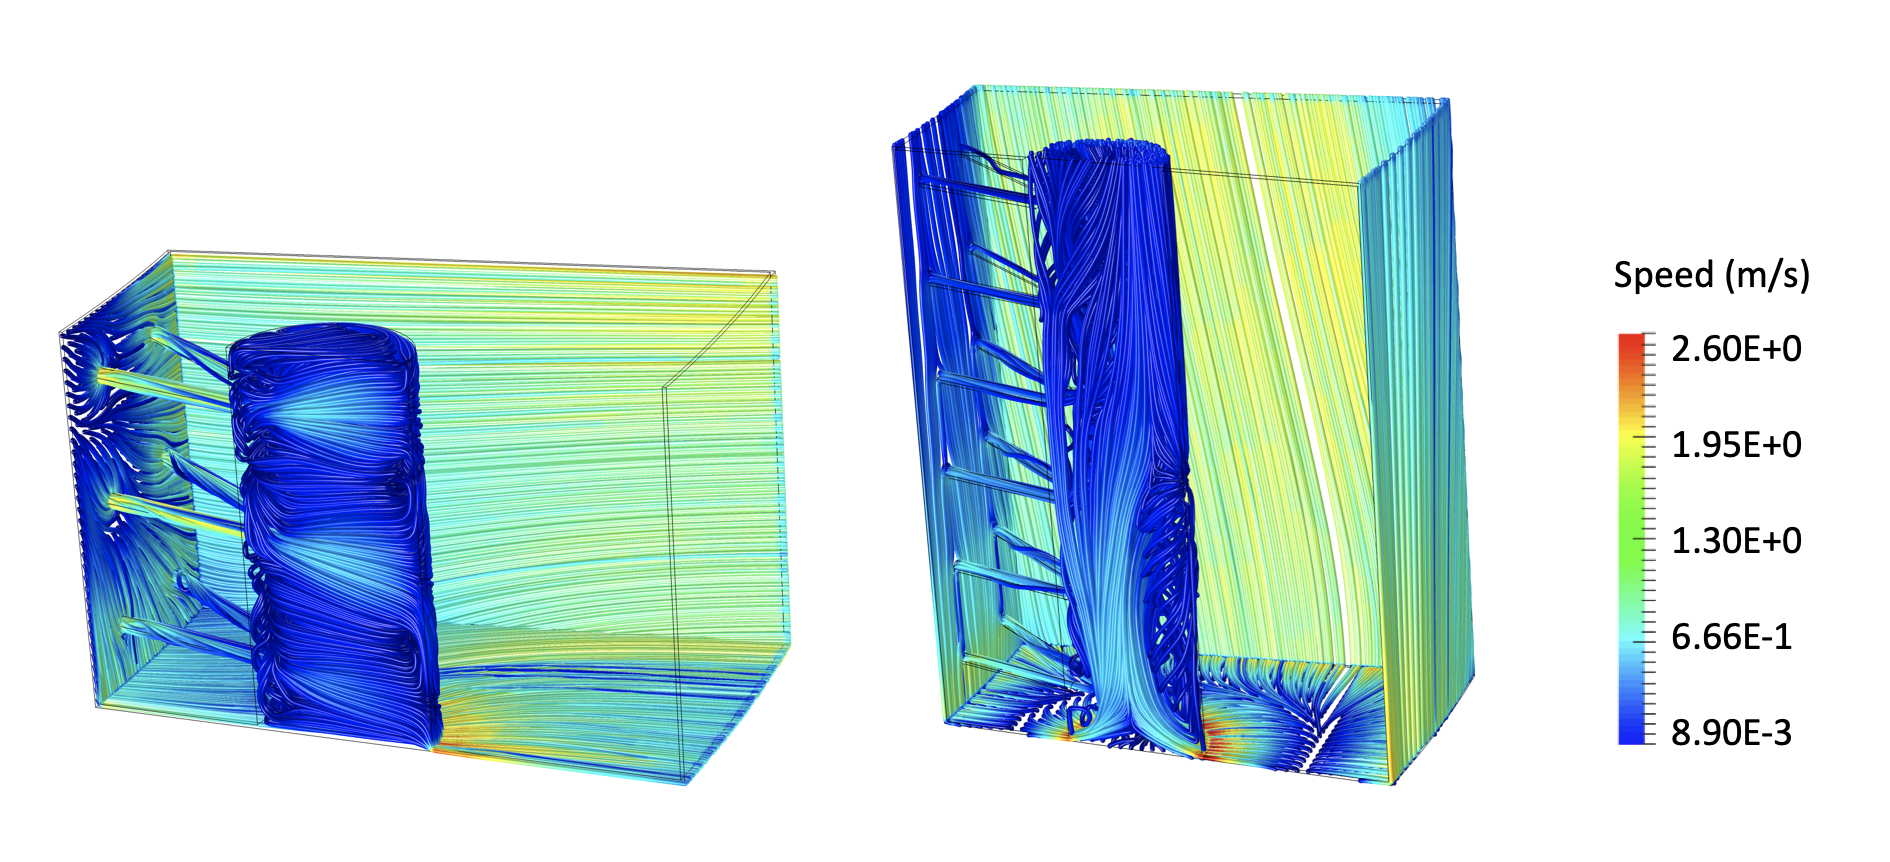
\includegraphics[width=0.8\linewidth]{figs/Re2000_cm05_U.png}
  \caption{\(Re=2000\)}
\end{subfigure}
\caption{COMSOL velocity predictions for a 5 \si{\milli\meter} gap at Reynolds numbers of (a) 500 and (b) 2000 for flow in the horizontal (left column) and vertical (right column) directions.}
\label{fig:velocity_5}
\end{figure}

Fig.\ \ref{fig:velocity_10} shows COMSOL predictions of the velocity streamlines for a 10 \si{\milli\meter} gap at Reynolds numbers of (a) 500 and (b) 2000 in the two flow directions. For each Reynolds number, the velocities are again shown on the same color scale. While the velocity predictions for the 5 and 10 \si{\milli\meter} gaps are quite similar, there are a number of small differences. To conserve mass, the 10 \si{\milli\meter} gap results in roughly half the peak velocity as the 5 \si{\milli\meter} gap. For the horizontal flow case, the larger gap size results in less ``undercutting'' of flow from the horizontal gaps to the vertical gaps, as evident by the streamline directions near the horizontal and vertical gap junction. For the vertical flow case, a larger gap size results in more streamlined vertical flow through the center channel.

\begin{figure}[!htb]
\centering
\begin{subfigure}{\textwidth}
  \centering
  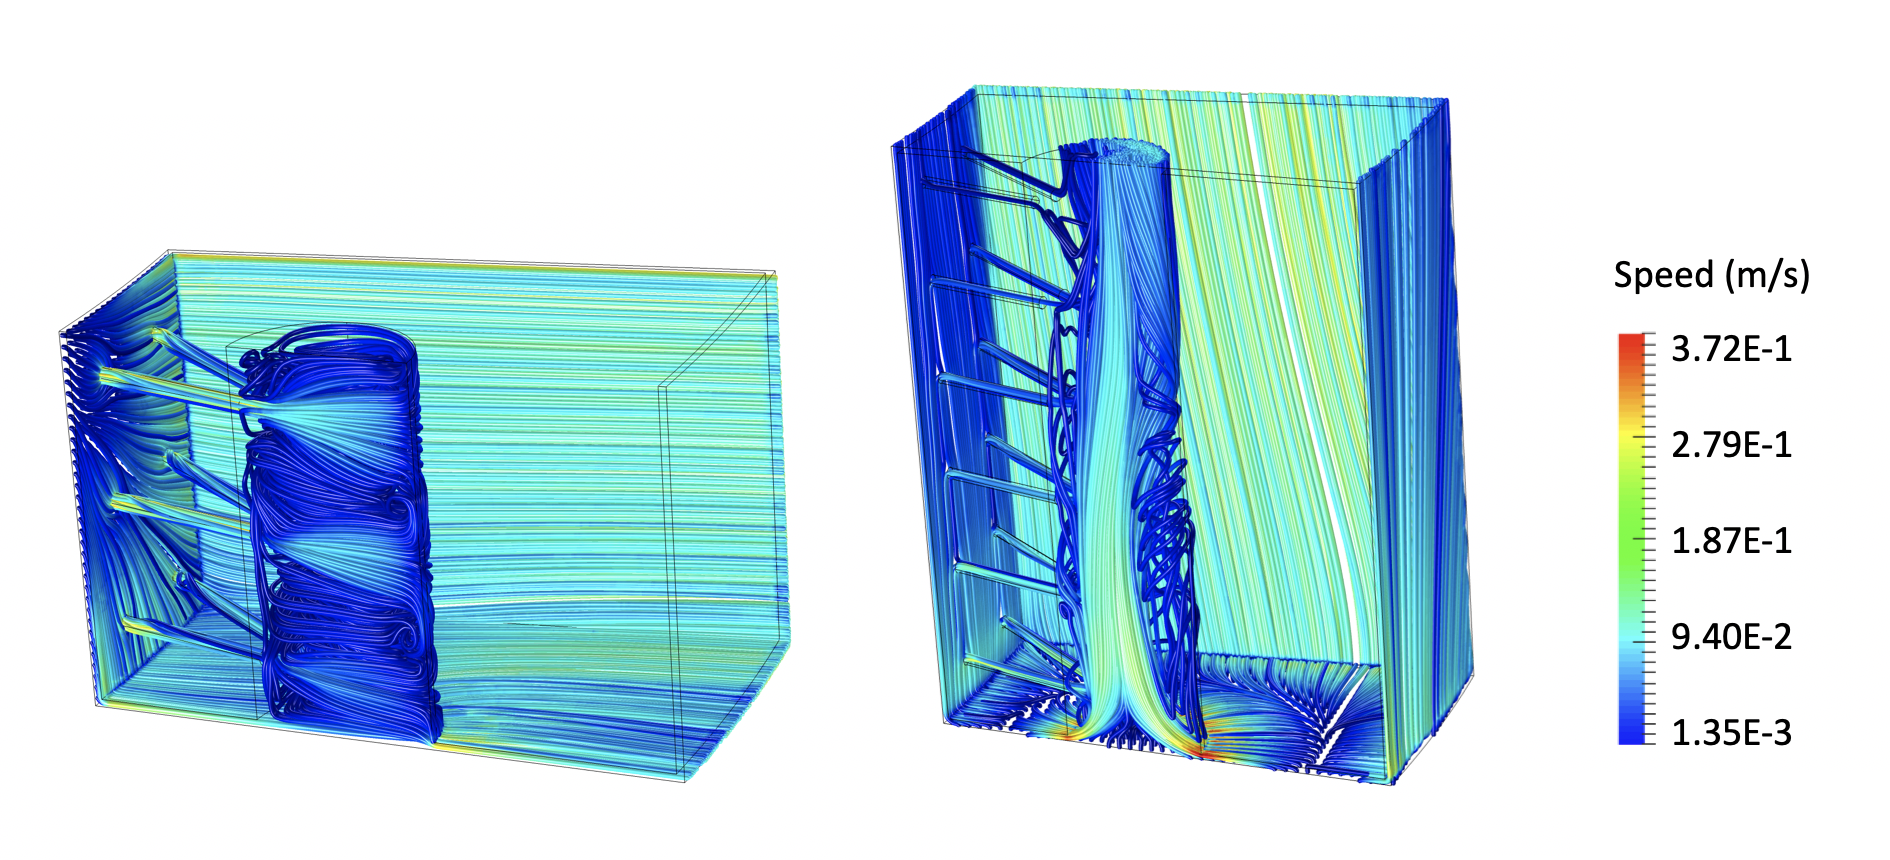
\includegraphics[width=0.8\linewidth]{figs/Re500_cm1_U.png}
  \caption{\(Re=500\)}
\end{subfigure}
\begin{subfigure}{\textwidth}
  \centering
  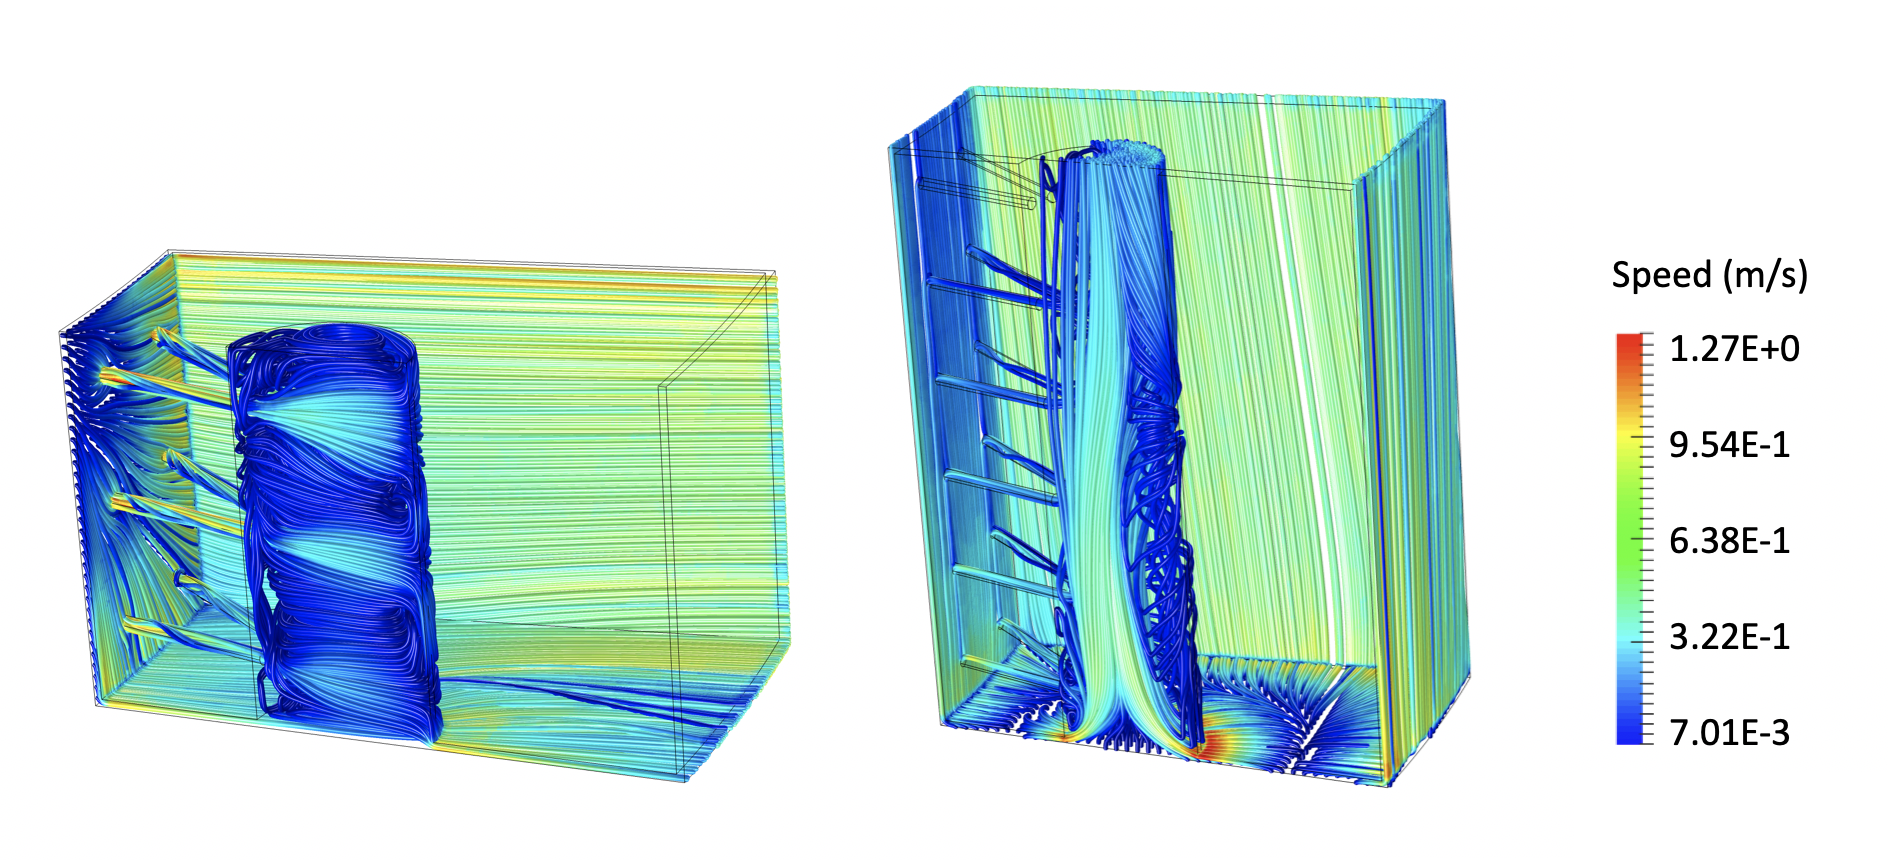
\includegraphics[width=0.8\linewidth]{figs/Re2000_cm1_U.png}
  \caption{\(Re=2000\)}
\end{subfigure}
\caption{COMSOL velocity predictions for a 10 \si{\milli\meter} gap at Reynolds numbers of (a) 500 and (b) 2000 for flow in the horizontal (left column) and vertical (right column) directions.}
\label{fig:velocity_10}
\end{figure}

Fig.\ \ref{fig:pressure_5} shows COMSOL predictions of the pressure for a 5 \si{\milli\meter} gap at Reynolds numbers of (a) 500 and (b) 2000 in the two flow directions. For each Reynolds number, the pressure is shown on the same color scale. For both the horizontal and vertical flow cases, most of the pressure drop occurs as the flow changes direction along the first perpendicularly-oriented no-slip face encountered. For the horizontal flow cases, the pressure is highest in the center of the inlet face and very low at the acceleration point where flow exits the vertical channel and enters the horizontal gap. For the vertical flow cases, the pressure is highest between the vertical coolant channel and the back-facing gap, with the highest stagnation pressure shifting closer to the coolant channel for higher Reynolds number.

\begin{figure}[!htb]
\centering
\begin{subfigure}{\textwidth}
  \centering
  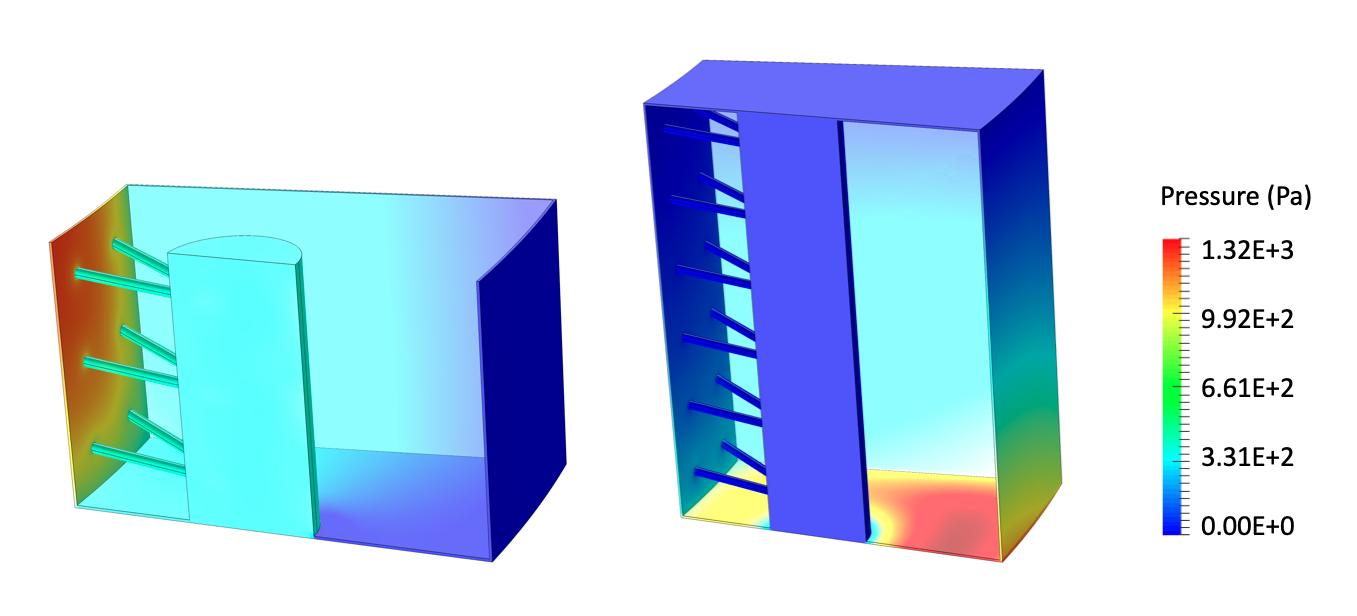
\includegraphics[width=0.8\linewidth]{figs/Re500_cm05_p.png}
  \caption{\(Re=500\)}
\end{subfigure}
\begin{subfigure}{\textwidth}
  \centering
  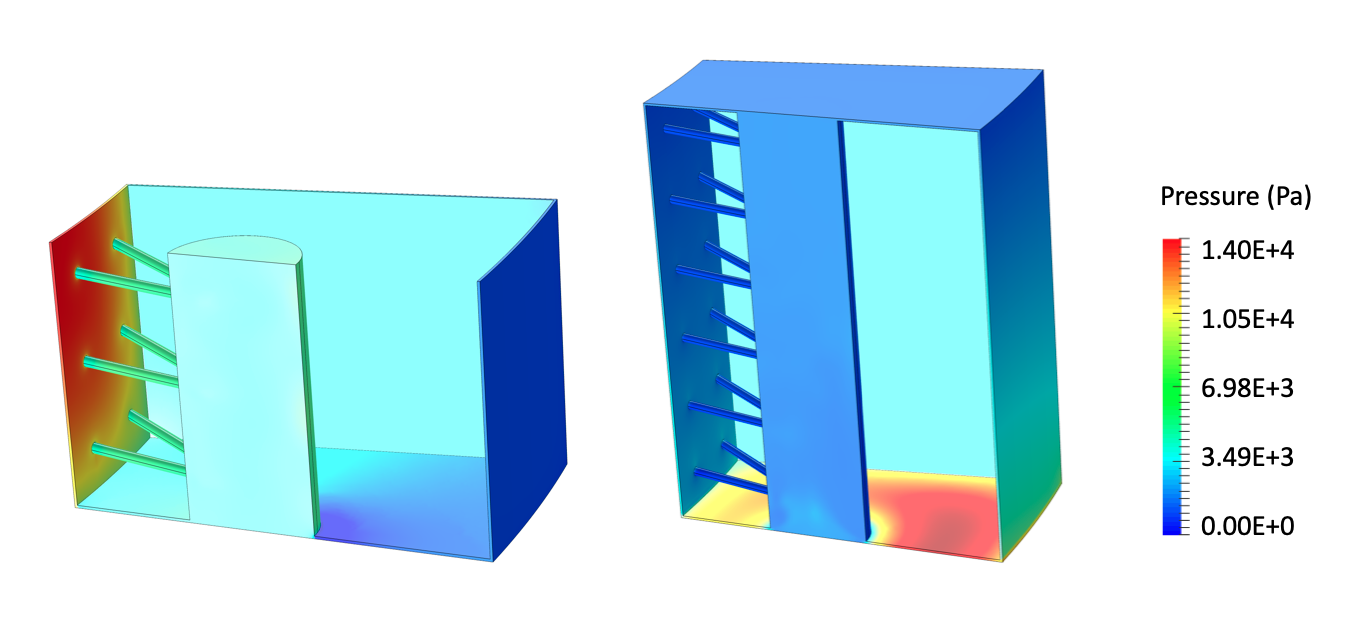
\includegraphics[width=0.8\linewidth]{figs/Re2000_cm05_p.png}
  \caption{\(Re=2000\)}
\end{subfigure}
\caption{COMSOL pressure predictions for a 5 \si{\milli\meter} gap at Reynolds numbers of (a) 500 and (b) 2000 for flow in the horizontal (left column) and vertical (right column) directions.}
\label{fig:pressure_5}
\end{figure}

Fig.\ \ref{fig:pressure_10} shows COMSOL predictions of the pressure for a 10 \si{\milli\meter} gap at Reynolds numbers of (a) 500 and (b) 2000 in the two flow directions. For each Reynolds number, the pressure is again shown on the same color scale. When normalized to the range \(\left\lbrack0, 1\right\rbrack\), the pressure distributions for the 5 and 10 \si{\milli\meter} gaps are very similar, especially for the vertical flow case. For the horizontal flow case and a larger gap size, the low-pressure region at the acceleration point between the vertical channel and the horizontally-oriented gap is more dispersed.

\begin{figure}[!htb]
\centering
\begin{subfigure}{\textwidth}
  \centering
  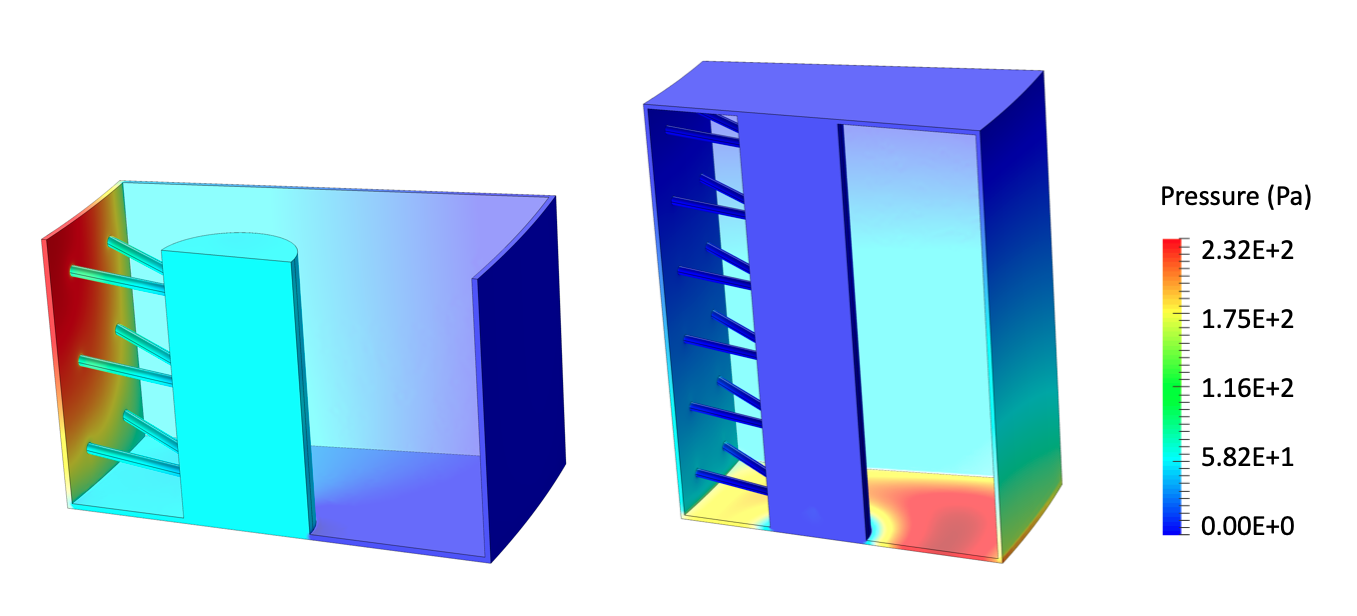
\includegraphics[width=0.8\linewidth]{figs/Re500_cm1_p.png}
  \caption{\(Re=500\)}
\end{subfigure}
\begin{subfigure}{\textwidth}
  \centering
  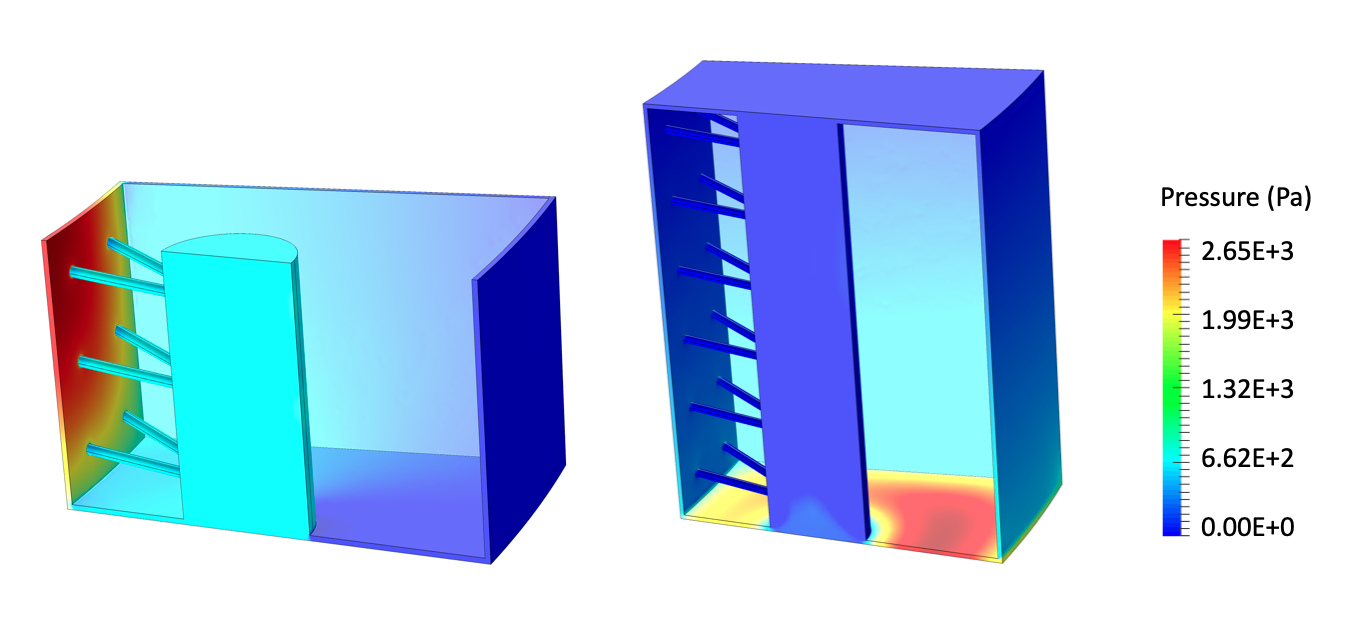
\includegraphics[width=0.8\linewidth]{figs/Re2000_cm1_p.png}
  \caption{\(Re=2000\)}
\end{subfigure}
\caption{COMSOL pressure predictions for a 5 \si{\milli\meter} gap at Reynolds numbers of (a) 500 and (b) 2000 for flow in the horizontal (left column) and vertical (right column) directions.}
\label{fig:pressure_10}
\end{figure}

Fig.\ \ref{fig:dp} shows the friction factor as a function of Reynolds number in the vertical and horizontal flow directions for the two gap sizes considered. For each gap size and flow direction, simulations were performed at eight Reynolds numbers except for the vertical flow case with the 5 \si{\milli\meter} gap, where the largest mesh size resulted in prohibitively long runtimes given project computing constraints. Solid markers represent \gls{cfd} data points and lines represent the friction factor fits with the form given in Eq. \eqref{eq:W3}. 

\begin{figure}[h!]
\centering
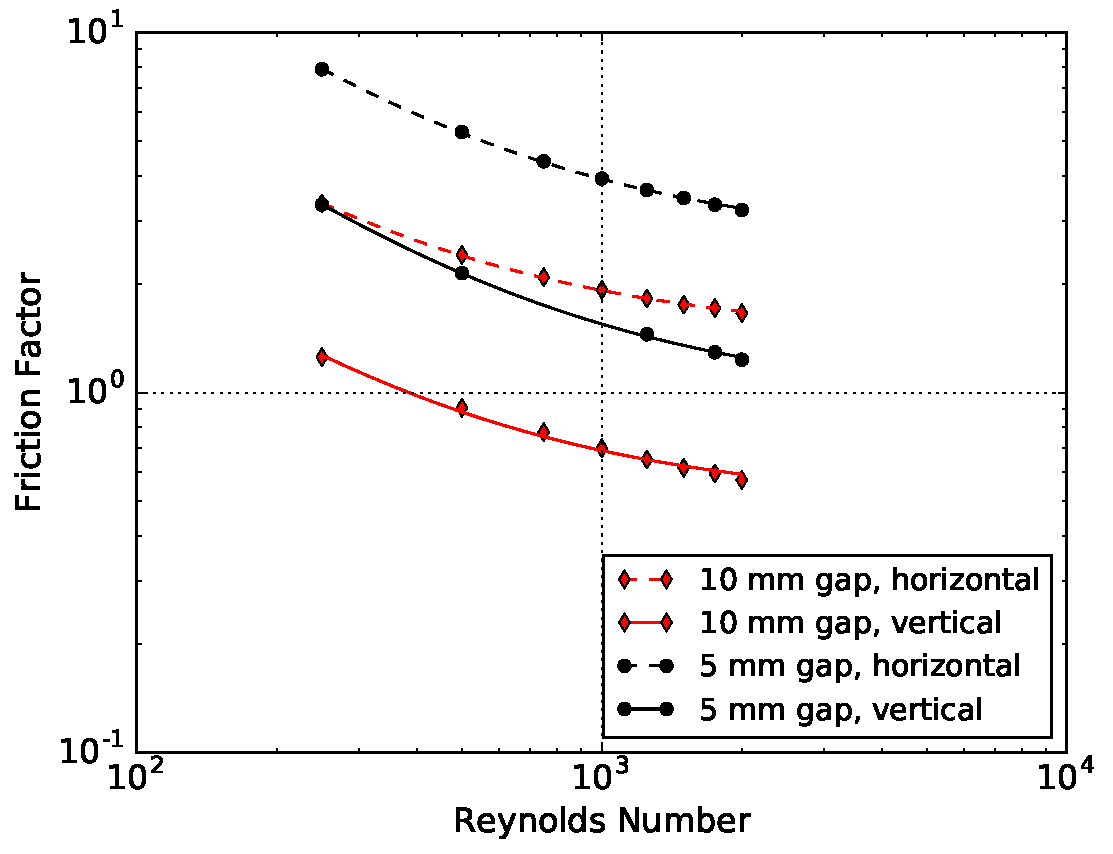
\includegraphics[width=0.6\linewidth]{figs/drag.pdf}
\caption{COMSOL predictions of the friction factor (discrete points) as a function of Reynolds number for 5 and 10 \si{\milli\meter} gaps. Continuous lines are fits to \gls{cfd} data with Eq. \eqref{eq:W3}.}
\label{fig:dp}
\end{figure}

Table \ref{table:drag} summarizes the \(A\) and \(B\) coefficients used to correlate the pressure drop with Eq. \eqref{eq:W3} for horizontal and vertical flows, respectively. The ``\(rr\)'' subscripts refer to the radial flow correlation and the ``\(zz\)'' subscripts refer to the axial flow correlation. The average and maximum percent error of the correlation with respect to the \gls{cfd} data points is on the order of several percent, indicating a good fit of the \gls{cfd} data to Eq. \eqref{eq:W3}.

\begin{table}[htb!]
\caption{Outer reflector friction factor correlations for radial and axial flow, with \(A_{ij}\) and \(B_{ij}\) defined in Eq. \eqref{eq:W3}. The error in the correlation is calculated relative to the \gls{cfd} data points.}
\centering
\small
\begin{tabular}{|c| c c c c | c c c c|}
\hline\hline
\multirow{2}{*}{Gap (\si{\milli\meter})} & \multirow{2}{*}{\(A_{rr}\)} & \multirow{2}{*}{\(B_{rr}\)} & Average & Maximum & \multirow{2}{*}{\(A_{zz}\)} & \multirow{2}{*}{\(B_{zz}\)} & Average & Maximum\Tstrut\\
& & & Error (\%) & Error (\%) & & & Error (\%) & Error (\%)\Bstrut\\
\hline
5.0 & 1337.76 & 2.58 & 0.47 & 1.09 & 593.78 & 0.96 & 0.65 & 1.50\Tstrut\\
10.0 & \color{white}0\color{black}479.38 & 1.44 & 0.43 & 1.17 & 193.47 & 0.50 & 1.90 & 3.82\Bstrut\\
\hline
\end{tabular}
\label{table:drag}
\end{table}

Because of the alignment of the largest coolant channel with the vertical direction, friction factors are larger in the radial direction than in the axial direction. At gap sizes of 5 and 10 \si{\milli\meter}, the radial friction factor is on average 151.8\% higher and 176.3\% higher, respectively, than the axial friction factor. Over the Reynolds number range investigated, the friction factor on average increases by 105.5\% and 125.7\% for the radial and axial directions, respectively, when the gap size decreases from 10 \si{\milli\meter} to 5 \si{\milli\meter}. Therefore, as the gap size is reduced, the axial friction factor increases faster than the radial friction factor.

It is important to revisit the assumptions made in the present drag correlation simulations to acknowledge sources of error and highlight the need for further study. Grooves on the block faces were neglected for ease of incorporating dimensional changes, while braided carbon fiber tubing was not considered since there was insufficient characterization in the available design documents. Accounting for these geometric details will likely result in different friction factors. Further, the one-equation Spalart-Allmaras turbulence model is used because of limited computational resources and the substantial geometric simplifications used in this work. 

From a more fundamental perspective, the pressure gradient was correlated in terms of a diagonal tensor with coefficients obtained from isolated simulations of flow in mutually orthogonal directions. Experiments are required to quantify the accuracy of this decomposition for the particular geometry considered. 

For both the vertical and horizontal flow cases, a uniform mass flux was imposed on the inlet face. For the vertical flow cases in particular, a uniform inlet flux is a significant simplification of the actual inflow that would be more heavily concentrated near the vertical coolant channel from the upstream block ring. If multiple stacked blocks were considered for the vertical direction, the flow entering the second block would  be more heavily concentrated near the mouth of the vertical coolant channel, reducing the fraction of flow stagnating on the bottom horizontal surface. The increase in streamlining with stacked blocks would therefore likely result in a reduction in the axial friction factors.

The \gls{bc} imposed at the bed-reflector interface should also account for the randomly-heaped pebble geometry, which has a significant effect on the flow distribution in this region \cite{amini}. Future work will repeat the \gls{cfd} correlation of outer reflector block friction factors with a two-equation turbulence model for multiple stacked blocks adjacent to a resolved pebble bed.

\section{Multiscale Core Analysis}
\label{sec:core}

This section combines the multiscale \gls{pbr} model described in Chapter \ref{sec:PhysicalModels} with the \gls{hsd} verification in Section \ref{sec:meso_fhr} and reflector block drag models in Section \ref{sec:bypass} to full-core, steady-state analysis of the \gls{pbfhr}. The heat source is specified with the sinusoidal axial distribution shown in Fig.\ \ref{fig:heat_source} to decouple the thermal physics from neutronics feedback.

\begin{figure}[h!]
\centering
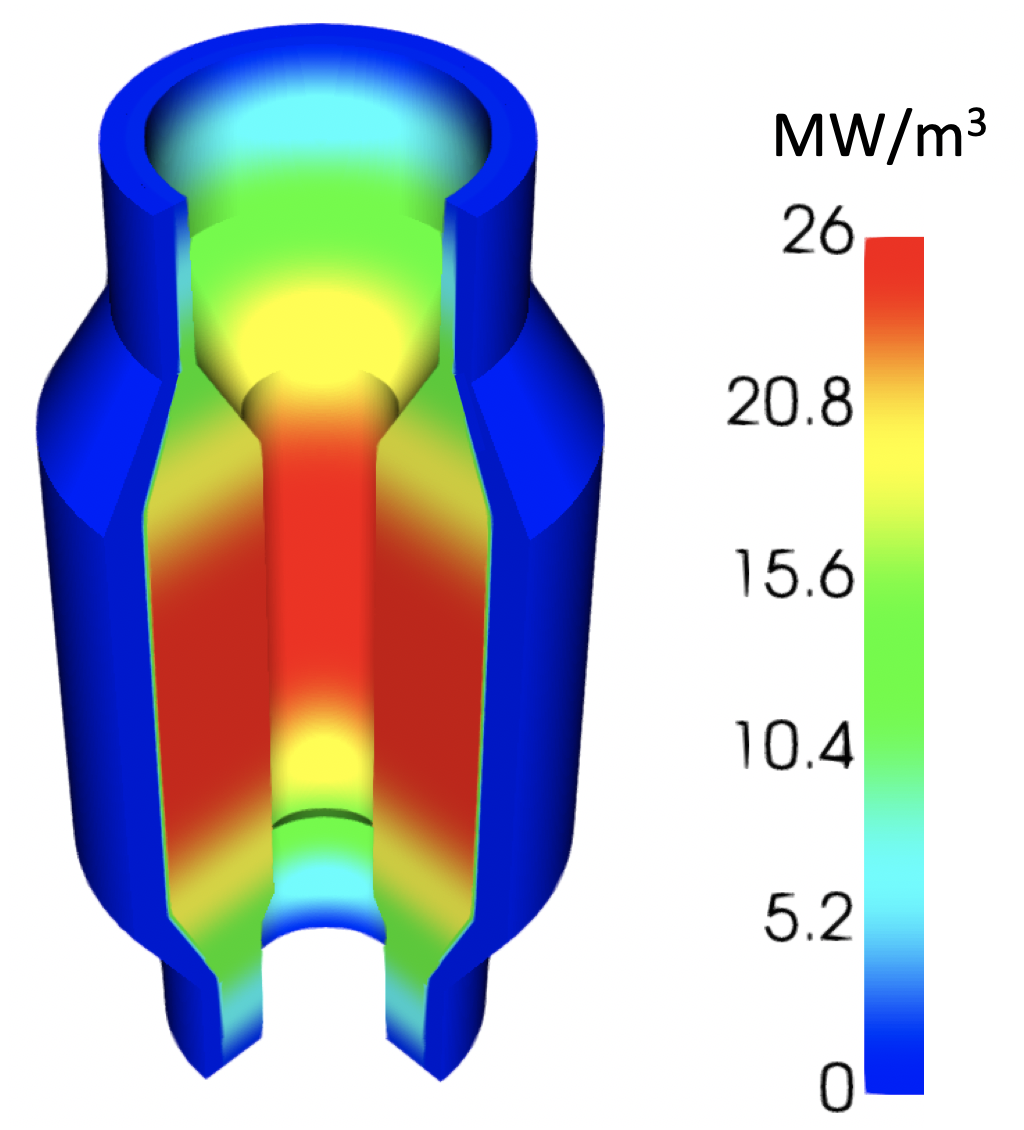
\includegraphics[width=0.375\linewidth]{figs/heat_source.png}
\caption{Volumetric heat source \(\dot{q}_s\) assumed for the \gls{pbfhr}.}
\label{fig:heat_source}
\end{figure}

Several different analyses are performed to demonstrate the multiscale model developed in Chapter \ref{sec:PhysicalModels} and predict \gls{th} phenomena of interest to reactor design. In Section \ref{sec:inflow}, a number of different inflow \glspl{bc} are evaluated from the perspective of the end-of-life bypass fraction, outlet fluid temperature distribution, and pumping power. These three metrics are indicative of the thermal performance of the \gls{pbfhr}. 

The bypass fraction is related to bulk coolant diversion from the pebble bed, which is expected to uniformly increase pebble temperatures and the proximity to \gls{cfp} failure limits. The maximum and mass-flux-weighted fluid temperature on the plenum inlet are indicative of the highest temperatures expected in downstream structural materials, which are often limited by integrity concerns. For instance, the average outlet coolant temperature in the \gls{tmsrsf1} is limited to 730\si{\celsius}, the highest allowable usage temperature of Hastelloy N \cite{xiao}. If Hastelloy N comprises structural materials in the \gls{pbfhr} outlet plenum, the mass-flux-weighted fluid temperature on the plenum inlet must be below 730\si{\celsius} to ensure material integrity. Related to the bypass fraction, basic energy conservation implies that the outlet fluid temperature is roughly inversely proportional to the core mass flow rate; achieving a uniform and low outlet fluid temperature requires both low bypass and a judicious choice of inlet flow \gls{bc}. Closely related to the inflow \gls{bc}, in particular the combination of axial and radial inlets, the core pressure drop is an indication of pumping requirements. 

For a number of different reflector block gap distributions, an inflow \gls{bc} design that achieves low bypass, maximum and average outlet fluid temperatures, and pressure drop is recommended for more detailed analysis in Section \ref{sec:depth}. Multiscale predictions of fuel and blanket pebble temperature distributions provide additional insights into the effects of bypass and inflow \gls{bc} design on fuel and structural material temperature limits.

It should be emphasized that the primary purpose of this section is to demonstrate, by example application to the \gls{pbfhr}, a multiscale model applicable to salt-cooled \glspl{pbr}. Therefore, the predictions given in Sections \ref{sec:inflow} and \ref{sec:depth} should be understood as preliminary and subject to revision upon more refined design information. 

\subsection{Inflow Conditions and Core Bypass}
\label{sec:inflow}

This section demonstrates macroscale analysis of the \gls{pbfhr} with a number of different inflow \glspl{bc} to investigate 1)~how the inlet flow \gls{bc} affects the fluid temperature distribution and bypass fraction and 2)~recommend an inlet \gls{bc} that achieves a balance between minimizing the bypass fraction, maximum and average fluid temperature on the plenum inlet, and core pressure drop. A number of different reflector block gap sizes are considered to understand how the bypass fraction varies with reflector dimensional changes and whether inflow \gls{bc} design optimization must consider variation in bypass over reflector lifetime.

Because flow exchanges between the bed and the reflectors via gaps and the horizontal coolant channels, the bypass fraction can be defined several different ways. Two colored dashed lines are shown in Fig.\ \ref{fig:pbfhr_slice} to aid in this description. The ``inlet'' bypass fraction is defined as the fraction of the total mass flow that enters the bottom of the outer reflector, or along the surface indicated with a green dashed line. Some of this flow may re-enter the bed, so the inlet bypass fraction does not necessarily represent the fraction of flow that bypasses the pebbles. Instead, the ``total'' bypass fraction is calculated as the fraction of the total mass flow that bypasses the surfaces indicated with red dashed lines. This flow evades most of the pebble bed, and is considered a more representative measure of the bypass fraction.

Three different inner reflector flow \gls{bc} are considered in this section; each specifies the same total mass flow from the inner reflector, but differs in the axial variation. These \glspl{bc} are referred to as conditions A, B, and C, and are illustrated in Fig.\ \ref{fig:bcs}; the length of the black arrows roughly correspond to the magnitude of the mass flux at the indicated axial position. Not shown are the inflow \glspl{bc} on the bottom of the pebble bed and outer reflector, which are selected based on equalizing the core and reflector pressure drop as described in Section \ref{sec:pbfhr_model}.

\begin{figure}[!htb]
\centering
\begin{subfigure}{.32\textwidth}
  \centering
  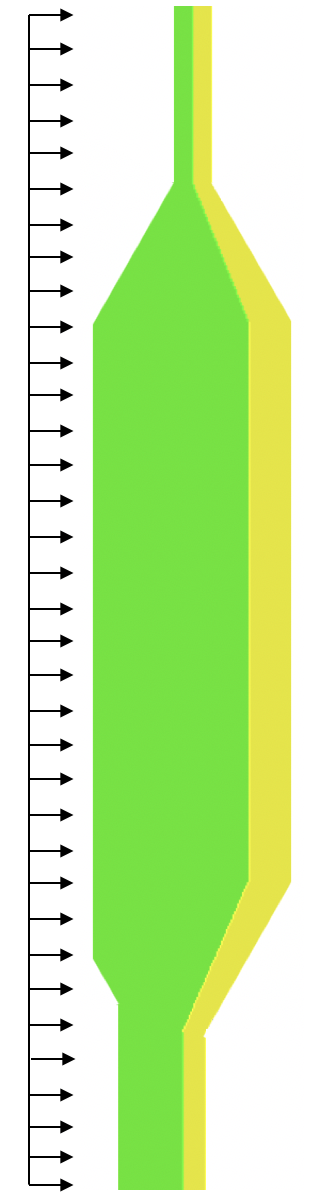
\includegraphics[height=1.5\linewidth]{figs/bc_A.png}
  \caption{Condition A}
\end{subfigure}
\begin{subfigure}{.32\textwidth}
  \centering
  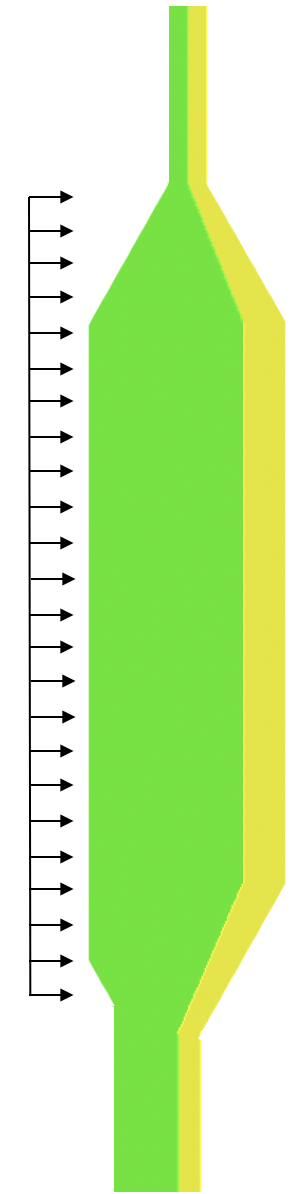
\includegraphics[height=1.5\linewidth]{figs/bc_B.png}
  \caption{Condition B}
\end{subfigure}
\begin{subfigure}{.32\textwidth}
  \centering
  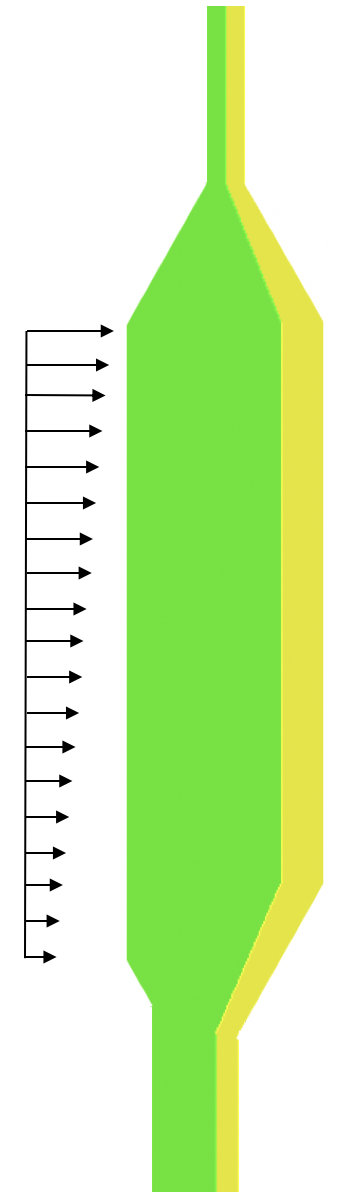
\includegraphics[height=1.5\linewidth]{figs/bc_C.png}
  \caption{Condition C}
\end{subfigure}
\caption{Illustration of three different inner reflector flow \glspl{bc} considered for the \gls{pbfhr}. The left axis of each figure is the $r$-$z$ symmetry axis. Condition C is shown for \(m>1\).}
\label{fig:bcs}
\end{figure}

Condition A sets a uniform mass flux along the entire reflector height, while condition B sets a uniform mass flux only along the centermost vertical and angled regions of the bed. Condition C sets a linear variation with height along the centermost vertical region, or

\beq
\label{eq:MassFluxBC}
\rho_f\vec{V}=\tilde{A}z+\tilde{B}\ ,
\eeq

\noindent where \(z\) is the vertical coordinate and \(\tilde{A}\) and \(\tilde{B}\) are constants selected to obtain 1)~the required total mass flow and 2)~\(m\) times higher mass flow at the top than the bottom. In other words, if the $z$-coordinate joining the vertical and upper slanted faces of the inner reflector is \(z_1\) and the $z$-coordinate joining the vertical and lower slanted faces of the inner reflector is \(z_0\), \(\tilde{A}\) and \(\tilde{B}\) are defined to satisfy

\begin{subequations}
\begin{align}
\label{eq:MFBC1}
\tilde{A}z_1+\tilde{B}=&\ m\left(\tilde{A}z_0+\tilde{B}\right)\\
\dot{m}_\text{ir}=&\ 2\pi\int_{z_0}^{z_1}\left(\tilde{A}z+\tilde{B}\right)dz\ ,
\end{align}
\end{subequations}

\noindent where \(\dot{m}_\text{ir}\) is the mass flowrate entering the bed from the inner reflector, or 70\% of the total mass flow of 976 \si{\kilo\gram\per\second}.

Three different values of \(m\) are considered\mdash \(m=0.2\), which represents a \(5\times\) larger mass flux at the bottom than at the top; \(m=1.0\), which represents uniform mass flux; and \(m=5.0\), which represents a \(5\times\) larger mass flux at the top than at the bottom. To differentiate between different values of \(m\), condition C is subscripted with the value of \(m\). For example, \(C_{5.0}\) represents condition C with \(m=5.0\). Therefore, a total of five \glspl{bc} with three underlying axial distributions are considered\mdash conditions A, B, C$_\text{0.2}$, C$_\text{1.0}$, and C$_\text{5.0}$.

For each inflow \gls{bc}, three different reflector block gap size distributions are considered\mdash uniform 5 \si{\milli\meter} gaps throughout the reflector, uniform 10 \si{\milli\meter} gaps throughout the reflector, and a linear interpolation of 5 and 10 \si{\milli\meter} gaps with the piecewise sinusoidal axial distribution shown in Fig.\ \ref{fig:axial_gaps}. This distribution, which is referred to as the ``axial'' distribution, approximates the dependence of block deformation on fast fluence by assuming larger gaps near the core axial mid plane where the power density is largest. Representing the sinusoidal power density function generically as \(f(z)\), the \(A\) and \(B\) drag coefficients in the sinusoidal region are computed as

\begin{equation}
A_{ij}=f(z)A_{ij,10}+\left\lbrack1-f(z)\right\rbrack A_{ij,5}\ ,
\end{equation}

\begin{equation}
B_{ij}=f(z)B_{ij,10}+\left\lbrack1-f(z)\right\rbrack B_{ij,5}\ ,
\end{equation}

\noindent where the ``5'' and ``10'' subscripts indicate drag coefficients correlated for the 5 and 10 \si{\milli\meter} uniform gaps, respectively. That is, the axial distribution linearly interpolates between the two gap sizes with a sinusoidal distribution. 

\begin{figure}[h!]
\centering
\hspace{1.5cm}
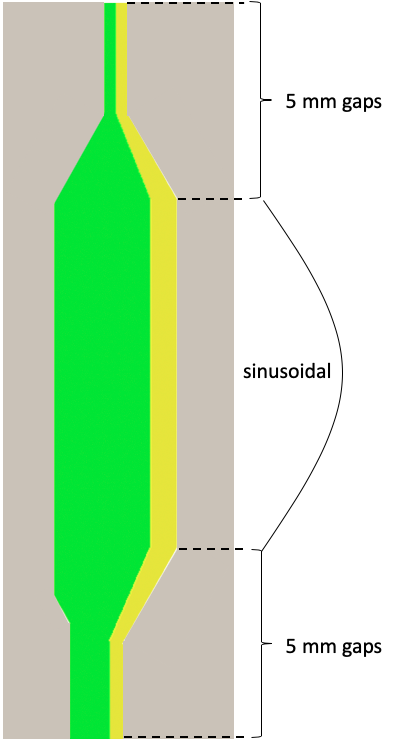
\includegraphics[width=0.255\linewidth]{figs/axial_gaps.png}
\caption{Axial gap size distribution used to approximate spatially-varying block deformation. The left axis is the $r$-$z$ symmetry axis.}
\label{fig:axial_gaps}
\end{figure}

It is important to note that uniform 10 \si{\milli\meter} gaps are likely unrealistically large, and \gls{th} predictions for this gap distribution should not be regarded as representative of the \gls{pbfhr} outer reflector end-of-life condition. Instead, the 10 \si{\milli\meter} gaps are considered to understand the sensitivity of bypass to the gap size and to contrast the axial distribution in Fig.\ \ref{fig:axial_gaps} with uniform distributions.

Figs. \ref{fig:bcs_temp}--\ref{fig:bcs_temp3} show the predicted fluid temperature and velocity streamlines in the pebble bed, plenum, and outer reflector for the five flow \glspl{bc} considered for 5 \si{\milli\meter} gaps, 10 \si{\milli\meter} gaps, and the axial gap distribution shown in Fig.\ \ref{fig:axial_gaps}, respectively. In each subfigure, the $r$-$z$ symmetry axis is on the left boundary and black arrows indicate the inner reflector flow \gls{bc}. Gray blocks represent the inner reflector, barrel, downcomer, and vessel. All temperatures in Figs. \ref{fig:bcs_temp}--\ref{fig:bcs_temp3} are shown on the same color scale.

For all \glspl{bc} and gap distributions, the bed is characterized by a combination of radial and axial flow. The horizontal component of velocity generally decreases moving towards the outer reflector because the drag is larger in the reflector than in the pebble bed. Flow in the outer reflector is primarily vertical, though flow enters the bed along the bottom slanted face adjacent to the outer reflector and shortly below the inlet to the outlet plenum to pass through the lower-resistance plenum instead of the higher-resistance reflector blocks.

The fluid temperature is highest near the core outlet due to the continual heating in the bed. The blanket graphite pebbles result in a thin stream of cool fluid along the interface between the bed and the outer reflector. Because heat transfer between the fluid and reflectors is neglected, the fluid temperature in the outer reflector and along the inner reflector surface matches the inlet temperature. Including convective heat transfer between the fluid and reflector blocks will result in higher fluid temperatures in both the inner and outer reflectors.

\begin{figure}[!htb]
\centering
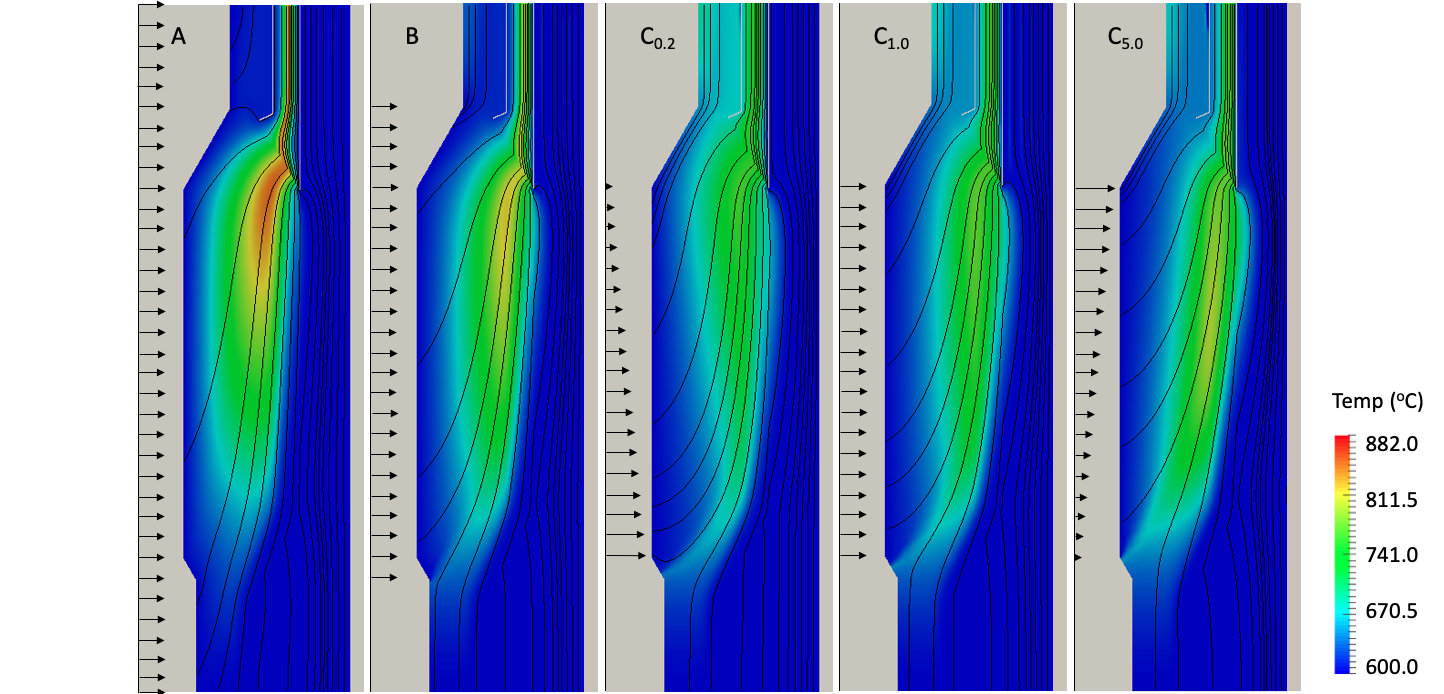
\includegraphics[width=0.85\linewidth]{figs/fluid_temp_05.png}
\caption{Predicted fluid temperature and velocity streamlines for a 5 \si{\milli\meter} reflector gap.}
\label{fig:bcs_temp}
\end{figure}

\begin{figure}[!htb]
\centering
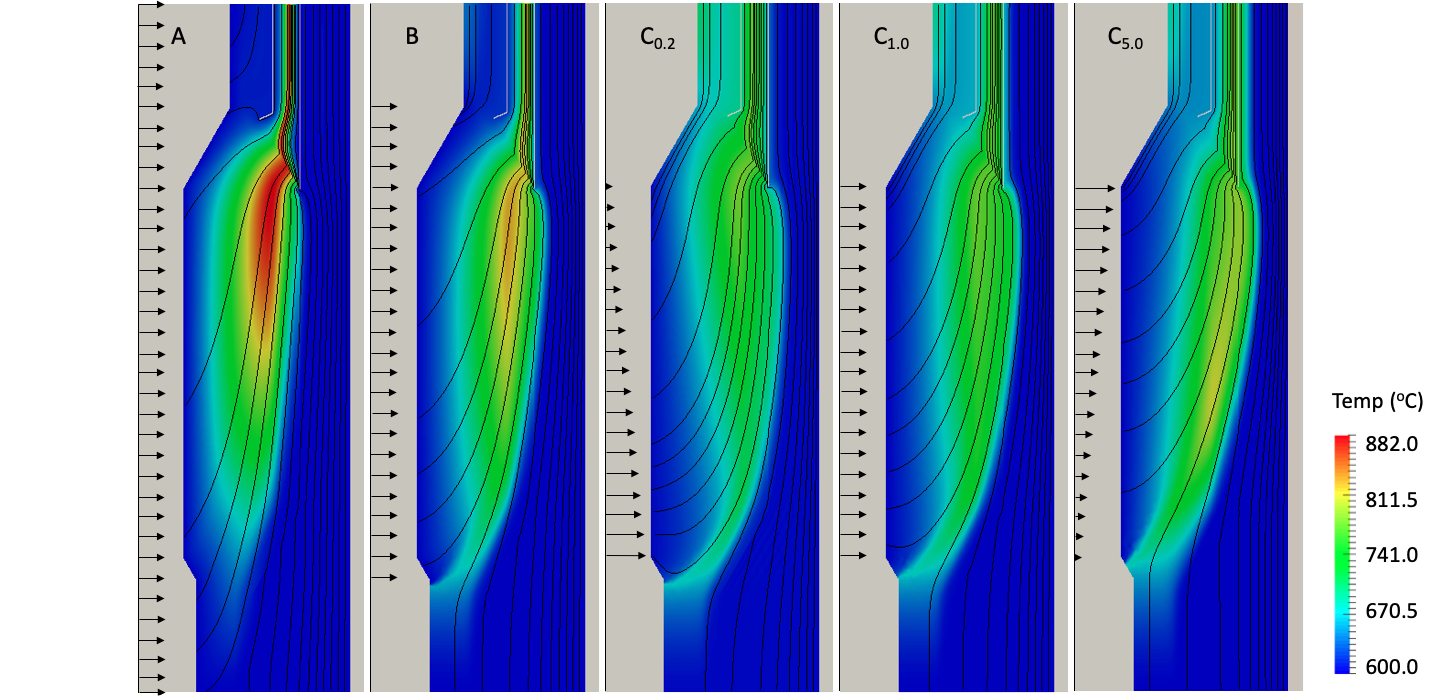
\includegraphics[width=0.85\linewidth]{figs/fluid_temp_1.png}
\caption{Predicted fluid temperature and velocity streamlines for a 10 \si{\milli\meter} reflector gap.}
\label{fig:bcs_temp2}
\end{figure}

\begin{figure}[!htb]
\centering
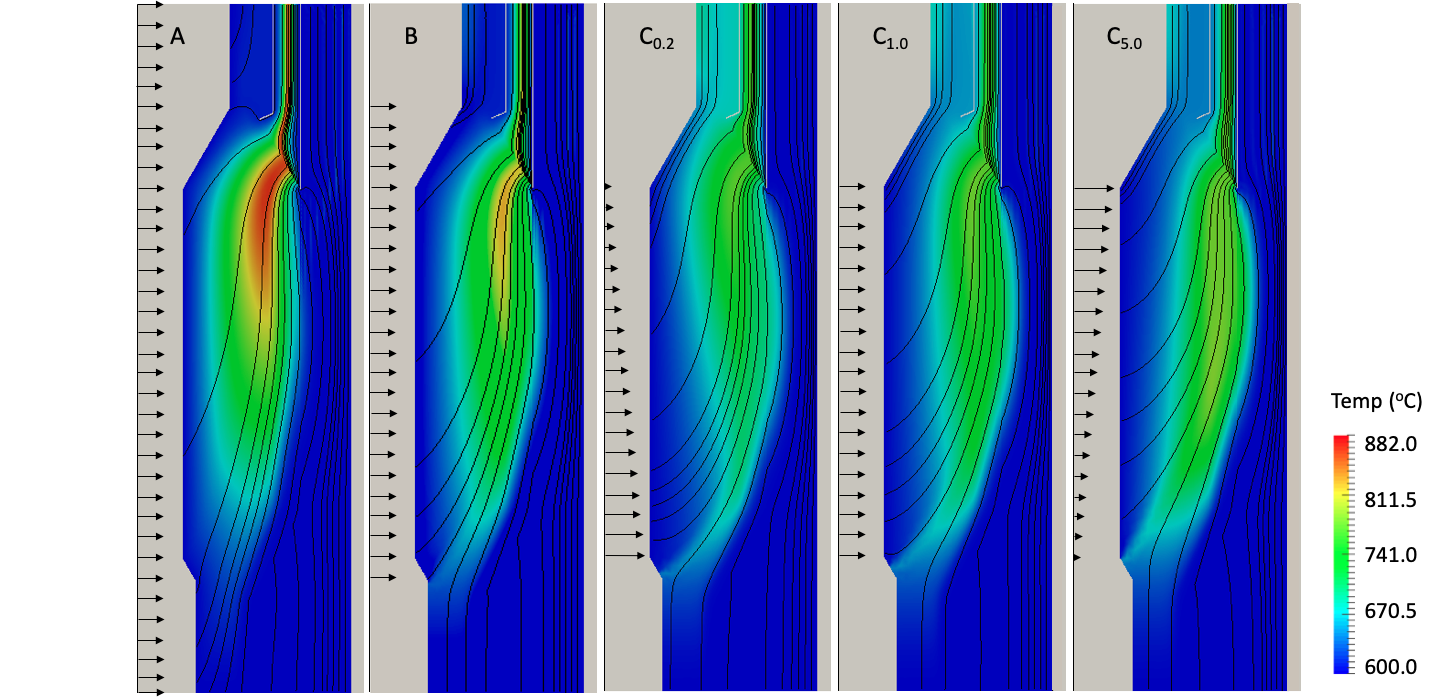
\includegraphics[width=0.85\linewidth]{figs/fluid_temp_axial.png}
\caption{Predicted fluid temperature and velocity streamlines for the axial reflector gap distribution shown in Fig.\ \ref{fig:axial_gaps}.}
\label{fig:bcs_temp3}
\end{figure}

Table \ref{table:drag3} summarizes the bypass fraction, the maximum and mass-flux-weighted fluid temperature on the plenum inlet, and the core pressure drop for the three gap distributions and five inflow \glspl{bc} considered. Note that the fluid temperature measurements correspond to the plenum inlet along the upper angled portion of the bed. The mass-flux-weighted fluid temperature along all core outlets, including the top of the outer reflector, is slightly below the nominal 700\si{\celsius} outlet temperature due to minor heat losses to the \gls{rrcls} system.

To interpret the data in Table \ref{table:drag3}, some general observations are first made with regards to all gap sizes and flow \glspl{bc}. For all cases, the inlet bypass fraction is higher than the total bypass fraction because some fluid flows into the bed from the reflector, especially near the angled boundary at the bottom fueling chute. When averaged over the different inflow conditions and gap sizes, approximately 3\% of the total mass flow enters the bed from the outer reflector. 

The core pressure drop is fairly insensitive to the gap size and inflow condition. The pumping power \(\mathcal{P}\) is the power required to overcome frictional and gravitational pressure losses in a loop system, and is defined as

\begin{equation}
\label{eq:PumpingPower}
\mathcal{P}\equiv\frac{\dot{m}}{\rho_f}\Delta P\ ,
\end{equation}

\noindent where \(\dot{m}\) is the core mass flowrate and \(\Delta P\) is the core pressure drop. Averaged over all cases, a core pressure drop of 1.15 atm results in a pumping power of approximately 58 kW, approximately one to two orders of magnitude smaller than characteristic of gas-cooled \glspl{pbr} and liquid-metal reactors.

\begin{table}[htb!]
\caption{Predicted core bypass, pressure drop, and maximum and mass-flux-weighted average fluid temperature along the plenum inlet as a function of inflow \gls{bc} and outer reflector gap size. The bolded lines correspond to the \gls{bc} selected for further study in Section \ref{sec:depth}.}
\centering
\small
\centerline{
\begin{tabular}{|c |c| c c |c| c c |}
\hline\hline
\multirow{2}{*}{Gap} & \multirow{2}{*}{Inflow BC} & Total & Inlet & $\Delta P$ & Average & Maximum  \Tstrut\\ %& Minimum & \(\mathcal{R}(T_f)\)
 & & Bypass (\%) & Bypass (\%) & (atm) & \(T_f\) (\si{\celsius}) & \(T_f\) (\si{\celsius}) \Bstrut\\ %& \(T_f\) (\si{\celsius}) & (\si{\celsius})
\hline
\multirow{5}{*}{5 \si{\milli\meter}} & A & 12.7 & 17.8 & 1.16 & 728.9 & 842.4\Tstrut\\ %& 612.0 & 230.4
& B & 11.9 & 15.1 & 1.16 & 717.9 & 804.0\\ %& 617.0 & 187.0
& \textbf{C$_{0.2}$} & \textbf{13.3} & \textbf{15.3} & \textbf{1.22} & \textbf{711.8} & \textbf{757.4}\\ %& \textbf{635.8} & \textbf{121.6}
& C$_{1.0}$ & 13.0 & 15.1 & 1.22 & 715.3 & 767.8\\ %& 649.8 & 116.0
& C$_{5.0}$ & 12.7 & 14.8 & 1.17 & 714.1 & 772.0\Bstrut\\ %& 643.6 & 128.4
\hline
\multirow{5}{*}{10 \si{\milli\meter}} & A & 24.9 & 25.5 & 1.10 & 746.4 & 878.8\Tstrut\\ %& 613.6 & 265.2
& B & 21.9 & 24.0 & 1.10 & 735.0 & 817.8\\ %& 619.4 & 198.4
& \textbf{C$_{0.2}$} & \textbf{21.9} & \textbf{26.7} & \textbf{1.14} & \textbf{732.2} & \textbf{774.8}\\ %& \textbf{670.7} & \textbf{104.1} 
& C$_{1.0}$ & 21.8 & 26.1 & 1.12 & 732.2 & 771.1\\ %& 661.5 & 109.6
& C$_{5.0}$ & 21.6 & 26.2 & 1.11 & 728.4 & 782.1\Bstrut\\ %& 650.4 & 131.7
\hline % sinuosidal
\multirow{5}{*}{axial} & A & 13.2 & 17.9 & 1.14 & 729.9 & 859.8\Tstrut\\ %& & 
& B & 12.3 & 15.1 & 1.15 & 719.1 & 813.6\\
& \textbf{C$_{0.2}$} & \textbf{14.0} & \textbf{15.4} & \textbf{1.19} & \textbf{715.3} & \textbf{767.8}\\
& C$_{1.0}$ & 13.6 & 15.1 & 1.17 & 716.1 & 770.7\\
& C$_{5.0}$ & 13.3 & 15.0 & 1.15 & 716.6 & 773.6\Bstrut\\
%\hline % piecewise constant
%\multirow{5}{*}{axial} & A & 13.6 & 17.9 & 1.13 & 730.6 & 869.2\Tstrut\\ % & 603.5 & 265.7
%& B & 12.8 & 15.3 & 1.13 & 719.4 & 816.9 \\ %& 615.8 & 201.0
%& C$_{0.2}$ & 14.5 & 15.4 & 1.17 & 715.3 & 772.6 \\ %& 616.7 & 155.9
%& C$_{1.0}$ & 14.1 & 15.1 & 1.16 & 716.3 & 771.6 \\ %& 623.3 & 148.3
%& C$_{5.0}$ & 13.8 & 15.0 & 1.17 & 716.2 & 771.6 \Bstrut\\ %& 641.0 & 130.6
\hline
\end{tabular}
}
\label{table:drag3}
\end{table}

The inflow \gls{bc} has a significant effect on the bypass and outlet fluid temperature distribution. For a fixed gap distribution, varying the inflow \gls{bc} results in roughly a 0.025 range in bypass fraction, a 15\si{\celsius} range in average plenum inlet fluid temperature, and a 95\si{\celsius} range in maximum plenum inlet temperature. 

Conditions A and B result in the highest temperatures because a large fraction of the inner reflector flow is introduced in low-power regions towards the exit of the bed. By restricting the inlet flow to the central vertical section of the inner reflector via conditions C$_\text{0.2}$, C$_\text{1.0}$, and C$_\text{5.0}$, the maximum outlet fluid temperature decreases by roughly 90\si{\celsius} and 40\si{\celsius} relative to conditions A and B, respectively.  Among the three C condition variations, the linear variation in velocity from the inner reflector does not have a significant effect on the average outlet temperature, while lower values of \(m\) result in lower maximum outlet temperatures because the fluid path length through the bed is longer. 
 
Generally, a higher the bypass flow corresponds to higher average and maximum outlet fluid temperatures as coolant is diverted from the bed. However, for all gap distributions, condition C$_\text{1.0}$ has the same or higher total bypass fraction than condition B, but a significantly lower maximum outlet temperature because fluid is preferentially introduced near the highest-powered regions. This shows that the bypass fraction is not the sole determining factor of the maximum and average outlet fluid temperature. 

However, for a fixed inflow \gls{bc}, the bypass fraction is indicative of the maximum and average fluid outlet temperatures. The smaller the gap size, the higher the reflector flow resistance. Comparing the three gap distributions shows higher the reflector resistance causes lower maximum and average fluid outlet temperatures; decreasing the gap size from 10 \si{\milli\meter} to 5 \si{\milli\meter} lowers the maximum and average outlet fluid temperatures by approximately 20\si{\celsius}. For almost all inflow \glspl{bc}, the pressure drop and average and maximum outlet temperature for the axial distribution lies within the range predicted for uniform 5 \si{\milli\meter} gaps and uniform 10 \si{\milli\meter} gaps. This is expected due to the construction of the reflector drag models for the axial distribution as a linear interpolation of the 5 and 10 \si{\milli\meter} gap correlations. 
% one thing I'm noticing is that the analysis seems to be observational without causal explanation. I think this would all be strong if it were clearer what things are causal and what things are just associated indicators. Does that make sense? Also discussing why something is as expected (or not) and why it makes sense deepens the analysis. You do do both of these things some places. 

Uniform 10 \si{\milli\meter} gaps are likely unrealistically large, so either the uniform 5 \si{\milli\meter} gaps or the axial distribution may be considered representative of the reflector end-of-life condition, contingent on the accuracy of linear interpolation between uniform gap sizes used in the axial distribution. Depending on the inflow \gls{bc} and how the bypass is defined, the maximum bypass fraction for the \gls{pbfhr} is predicted in the range of 11.9 to 17.9\%. Though characterized by different bed and reflector designs, this range is in line with the 18\% bypass observed in the \gls{thtr} \cite{baumer} and bypass fractions on the order of 10\% predicted for the \gls{htrpm} \cite{jun,jun2011}.

While the axial distribution lies closer to the midpoint of the 5 and 10 \si{\milli\meter} distributions in terms of temperatures, the bypass fractions are nearly the same as predicted for uniform 5 \si{\milli\meter} gaps. This suggests that the bypass fraction is most sensitive to the drag coefficient at the bottom and top extremes of the bed. The lower fluence in these regions likely results in gaps smaller than 5 \si{\milli\meter} at end-of-life, and the bypass fractions in Table \ref{table:drag3} should be understood as upper bounds on the actual bypass fraction.

Based on the comparisons performed in this section, condition C$_{0.2}$ is recommended as the starting point for more refined design calculations for the \gls{pbfhr} because 1)~the core pressure drop differs by 7\% or less among the different \glspl{bc} considered; 2)~condition C$_\text{0.2}$ results in significantly lower maximum and average outlet temperatures than conditions A and B; and 3)~condition C$_\text{0.2}$ generally achieves a lower maximum and average outlet temperature than other values of \(m\). For condition C$_{0.2}$, the maximum bypass fraction is predicted in the range 13.3 to 15.4\%, depending on how the bypass is defined. Condition C$_{0.2}$ is highlighted in Table \ref{table:drag3} and explored in greater depth in Section \ref{sec:depth}.

\subsection{Core Analysis for an Optimized Inflow Condition}
\label{sec:depth}

This section provides in-depth core \gls{th} predictions for the three reflector gap distributions with the C$_\text{0.2}$ inflow condition. As discussed at the end of Section \ref{sec:inflow}, this inlet \gls{bc} is selected for more detailed analysis because the average and maximum outlet fluid temperatures are generally lower than for the other \glspl{bc} considered, with only minor differences in core pressure drop. Therefore, unless otherwise noted, all results presented in this section correspond to inflow condition C$_\text{0.2}$.

Fig.\ \ref{fig:fluid_temp_all} shows the fluid temperature with velocity streamlines for the three gap distributions; all temperatures are shown on the same color scale. While the same data is shown in Figs. \ref{fig:bcs_temp}--\ref{fig:bcs_temp}, excluding flow conditions A and B from the shared color scale enables clearer visualization. 

Because core bypass diverts coolant from the entirety of the bed, a higher bypass raises the fluid temperature nearly uniformly through the bed. This is evident in the qualitative similarity in the fluid temperature among the different reflector gap sizes shown in Fig.\ \ref{fig:fluid_temp_all}. Fluid temperature differences are primarily constrained to the magnitude, rather than distribution, especially when comparing the two uniform block gap sizes. For all gap distributions, fluid enters the bed from the outer reflector along the bottom slanted face. An exchanging core-reflector flow path also exists near the axial mid-plane; flow exits the bed to the lower-resistance blocks, flows upwards in the outer reflector through several blocks, and re-enters below the outlet plenum. This flow is most visible in the uniform 10 \si{\milli\meter} and axial gap distributions, where the resistance near the core mid-plane is lowest.

\begin{figure}[h!]
\centering
\hspace{1.2cm}
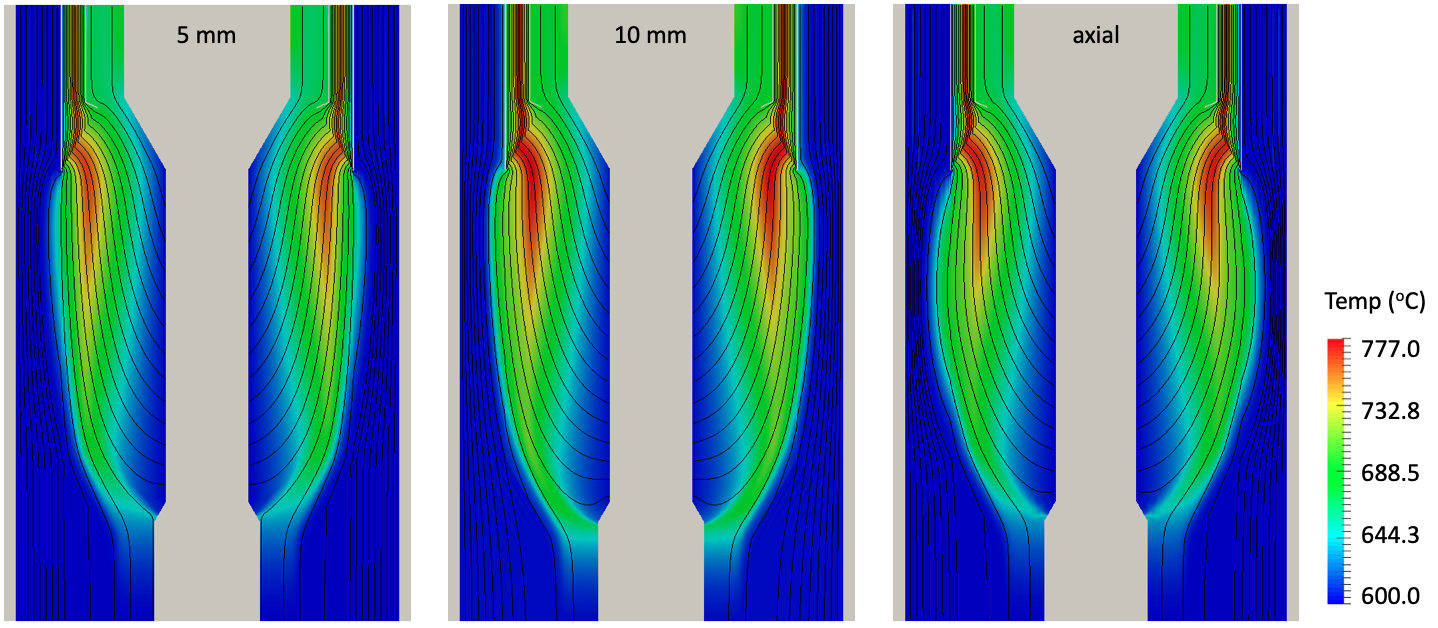
\includegraphics[width=0.9\linewidth]{figs/fluid_temp_all.png}
\caption{Predicted fluid temperature with velocity streamlines for inflow condition C$_\text{0.2}$ for all gap distributions.}
\label{fig:fluid_temp_all}
\end{figure}

For all gap distributions, the pressure drop is nearly linear with height; contours are primarily horizontal, with slight radial tilt near the plenum inlet. Fig.\ \ref{fig:pressure_all} shows the predicted pressure with contours in an inset in the pebble bed, plenum, and outer reflector for the 5 \si{\milli\meter} gap distribution. Because no significant difference is visible for the 10 \si{\milli\meter} and axial gap distributions aside from a slight shift in magnitude, the pressure predictions for the 10 \si{\milli\meter} and axial gap distributions are omitted for brevity. In Fig.\ \ref{fig:pressure_all}, the short dashed lines on the right face of the open 3-D rendering outline the pebble bed region. The discontinuities in the pressure contours near the top of the core occur over the thin solid walls encasing the outlet plenum.

\begin{figure}[h!]
\centering
\hspace{1.2cm}
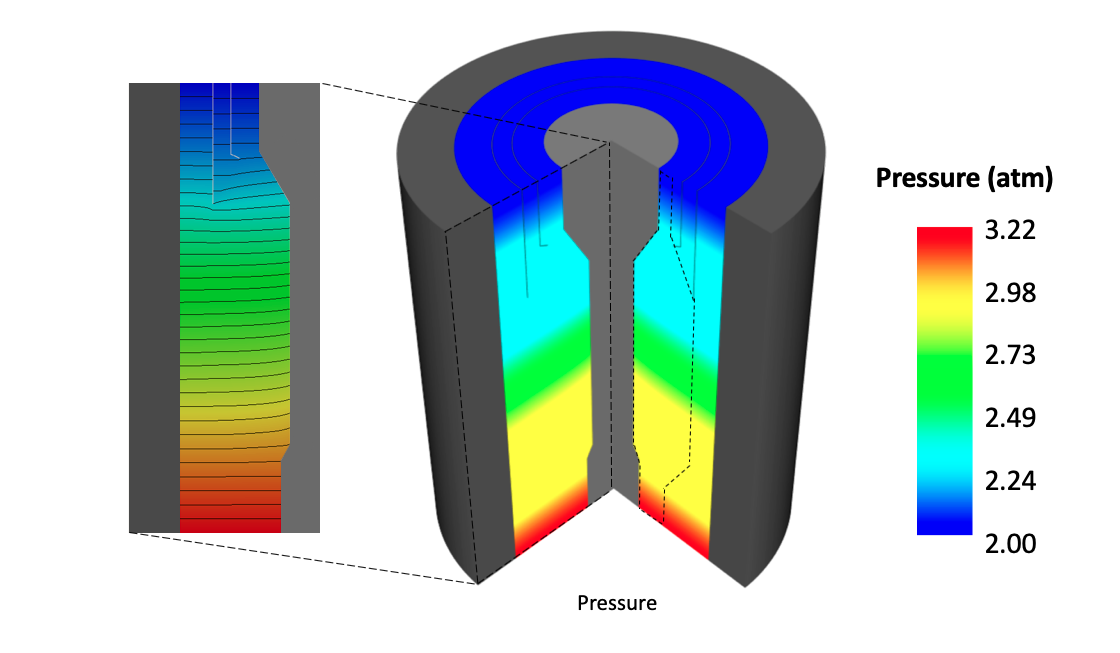
\includegraphics[height=0.4\linewidth]{figs/pressure_all.png}
\caption{Predicted pressure with contours for inflow condition C$_\text{0.2}$ for the 5 \si{\milli\meter} gap distribution. Short dashed lines outline the pebble bed region.}
\label{fig:pressure_all}
\end{figure}

For all three gap distributions, Fig.\ \ref{fig:solid_core} shows the predicted pebble surface temperature in the bed region and Fig.\ \ref{fig:solid_noncore} shows the solid temperature in the inner reflector, outer reflector, outlet plenum, barrel, downcomer, and vessel. The same color scale is used for Figs. \ref{fig:solid_core} and \ref{fig:solid_noncore}. The fire brick is excluded from the visualization in Fig.\ \ref{fig:solid_noncore} because the 600\si{\celsius} temperature drop from the vessel surface to the \gls{rrcls} system would saturate the color scale for visualization. The temperature contours in the firebrick are nearly vertical, as heat is conducted nearly entirely in the radial direction from the vessel surface.

The interface between the fuel and blanket pebbles is clearly visible in the pebble surface temperature distribution in Fig.\ \ref{fig:solid_core}. The combination of radial and axial coolant flow in the bed results in the highest temperatures occurring near the outlet of the bed and along the fuel-blanket interface due to a combination of higher coolant temperature and higher power density. Similar to the fluid temperatures shown in Fig.\ \ref{fig:fluid_temp_all}, the reflector gap profile and the resultant differences in core bypass primarily affect the magnitude of the solid surface temperature, rather than the distribution. 

The sharp line between fuel pebbles and blanket pebbles will in reality be smoothed from small amounts of pebble radial diffusion, while the sinusoidal power density does not account for radial peaking near reflectors \cite{xin_wang_thesis}. Both of these effects will be considered in future analyses.

\begin{figure}[h!]
\centering
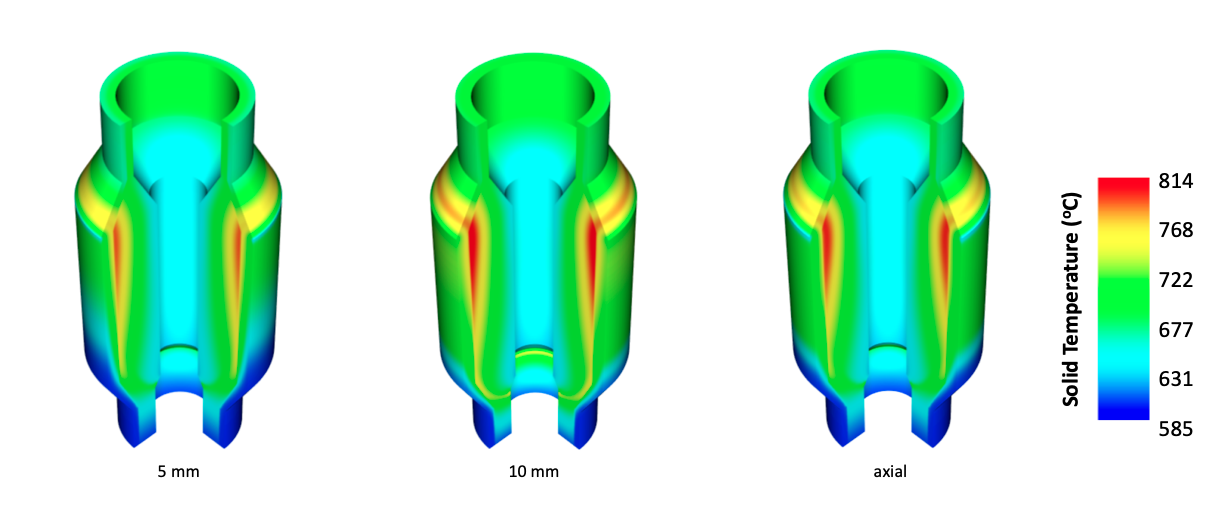
\includegraphics[height=0.4\linewidth]{figs/solid_temp_core.png}
\caption{Predicted pebble surface temperature for inflow condition C$_\text{0.2}$ for all gap distributions.}
\label{fig:solid_core}
\end{figure}

Heat conducts from the pebbles to the graphite reflectors and through the barrel, downcomer, vessel, and firebricks to removal by the \gls{rrcls} system. The highest reflector temperatures occur in the inner reflector and near the core outlet. As mentioned in reference to the fluid temperature distribution shown in Figs. \ref{fig:bcs_temp}--\ref{fig:bcs_temp3}, the omission of convective heat transfer between the fluid and reflectors overpredicts graphite temperatures in these regions. 
% did you give / do you have a sense of by how much? Or if this can be bounded? E.g. overpredicts by as much as 10%? It would help to get a rough sense of how big a deal this is. 
Future work involving generation of convective heat transfer closures for the \gls{pbfhr} reflector blocks is required to assess the magnitude of the effect on solid and fluid temperatures. Therefore, while the 10 \si{\milli\meter} gap results in the highest reflector temperatures in Fig.\ \ref{fig:solid_noncore}, the higher bypass flow may compensate by providing more heat removal than for the lower-bypass conditions.

\begin{figure}[h!]
\centering
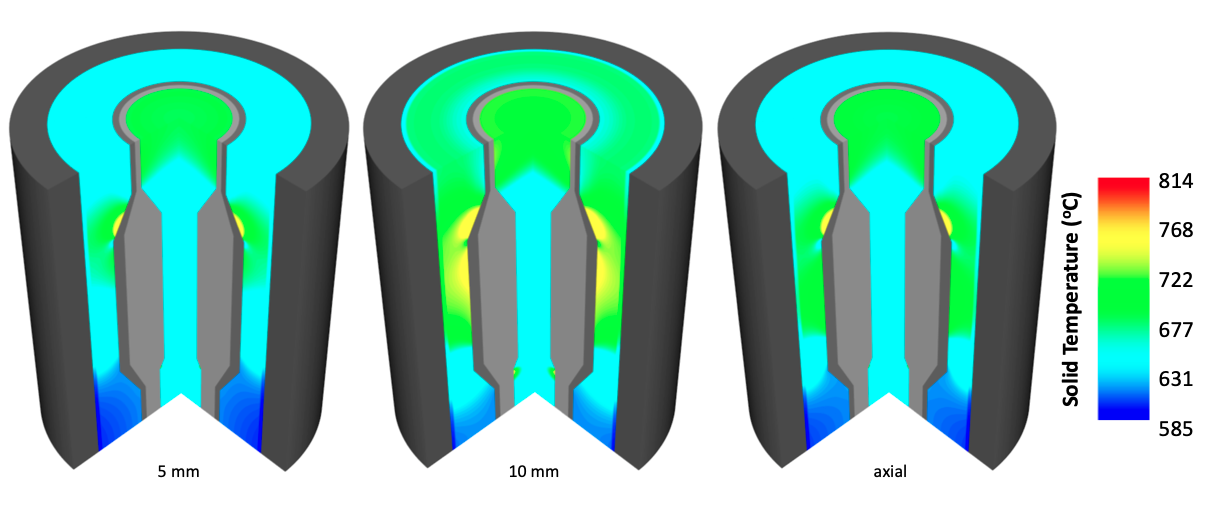
\includegraphics[height=0.4\linewidth]{figs/solid_temp_noncore.png}
\caption{Predicted solid temperature for inflow condition C$_\text{0.2}$ for all gap distributions.}
\label{fig:solid_noncore}
\end{figure}

For all three gap distributions, Figs. \ref{fig:uo2_max}, \ref{fig:uo2_avg}, and \ref{fig:graphite} show the maximum UC$_{1.5}$O$_{0.5}$ temperature in the fueled region, the average UC$_{1.5}$O$_{0.5}$ temperature in the fueled region, and the average graphite temperature in the bed, respectively. The same color scale is used in Figs. \ref{fig:uo2_max}--\ref{fig:graphite}.

The distribution of fissile kernel and graphite temperatures in the fuel pebble region is similar to the sinusoidal power density, but with maximum values shifted towards the right and slightly upwards in the core due to the combination of radial and axial flow inlets. The graphite temperature distribution in the blanket pebble region directly follows the fluid temperature distribution due to a lack of a volumetric heat source in this region.

The close proximity of \glspl{cfp} to the pebble surface results in roughly a 10\si{\celsius} difference between maximum and average kernel temperatures. Relative to gas-cooled designs with large central fuel-matrix regions, the \gls{pbfhr} pebble exhibits reduced pebble-wise temperature peaking. The maximum kernel temperature across all gap distributions is 880.1\si{\celsius}, far below the 1250\si{\celsius} limit for long-term operation of \gls{triso} particles \cite{nabielek,demkowicz}. Additional simulations under transient conditions are required to assess proximity to \gls{triso} particle failure temperatures for a wider set of possible operating states. 

\begin{figure}[h!]
\centering
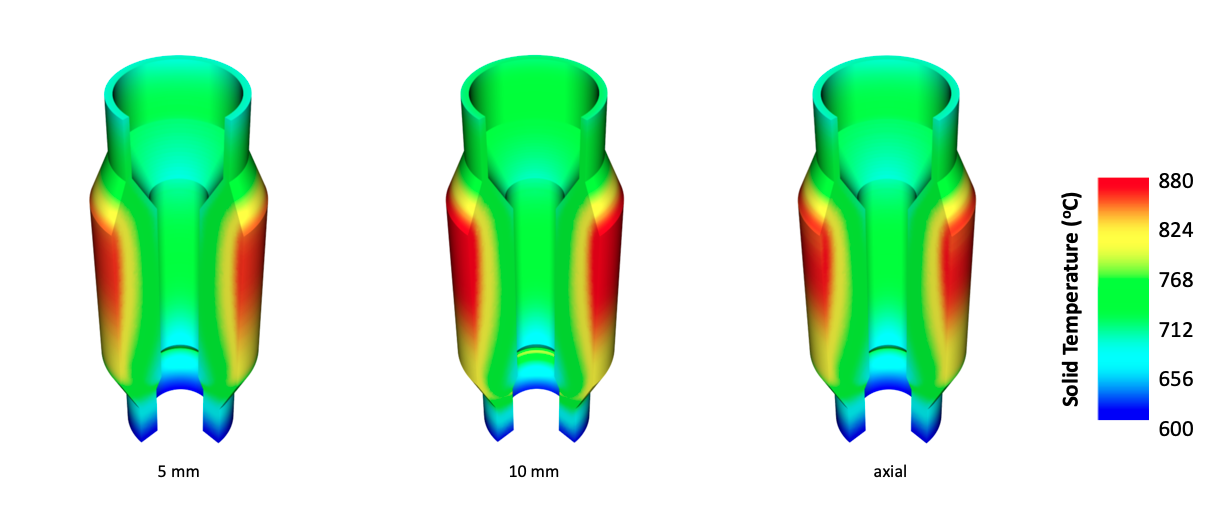
\includegraphics[height=0.4\linewidth]{figs/max_uo2.png}
\caption{Predicted maximum UC$_{1.5}$O$_{0.5}$ temperature for inflow condition C$_\text{0.2}$ for all gap distributions.}
\label{fig:uo2_max}
\end{figure}

\begin{figure}[h!]
\centering
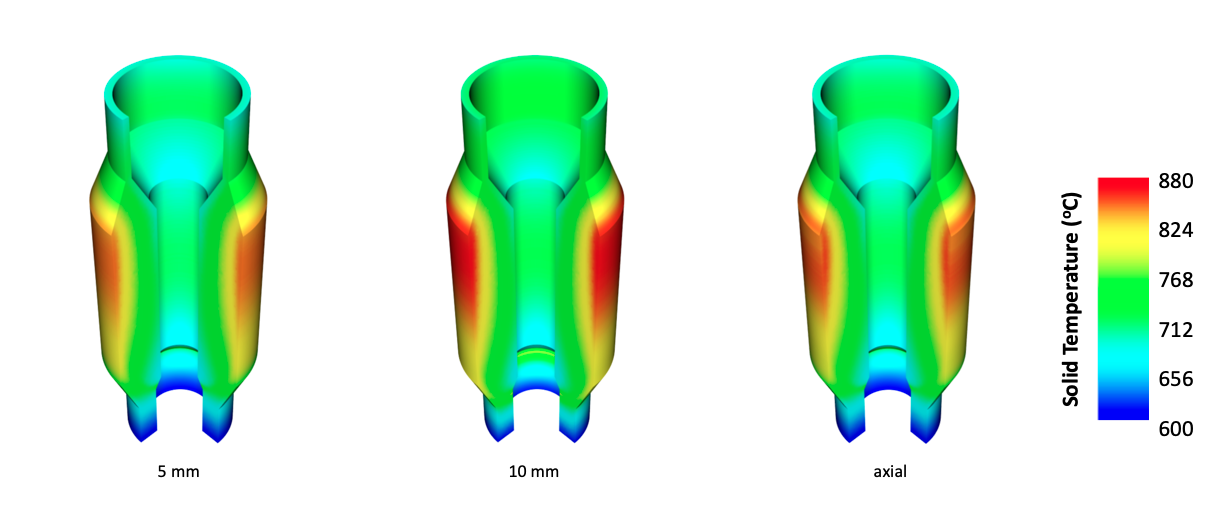
\includegraphics[height=0.4\linewidth]{figs/avg_uo2.png}
\caption{Predicted maximum UC$_{1.5}$O$_{0.5}$ temperature for inflow condition C$_\text{0.2}$ for all gap distributions.}
\label{fig:uo2_avg}
\end{figure}

\begin{figure}[h!]
\centering
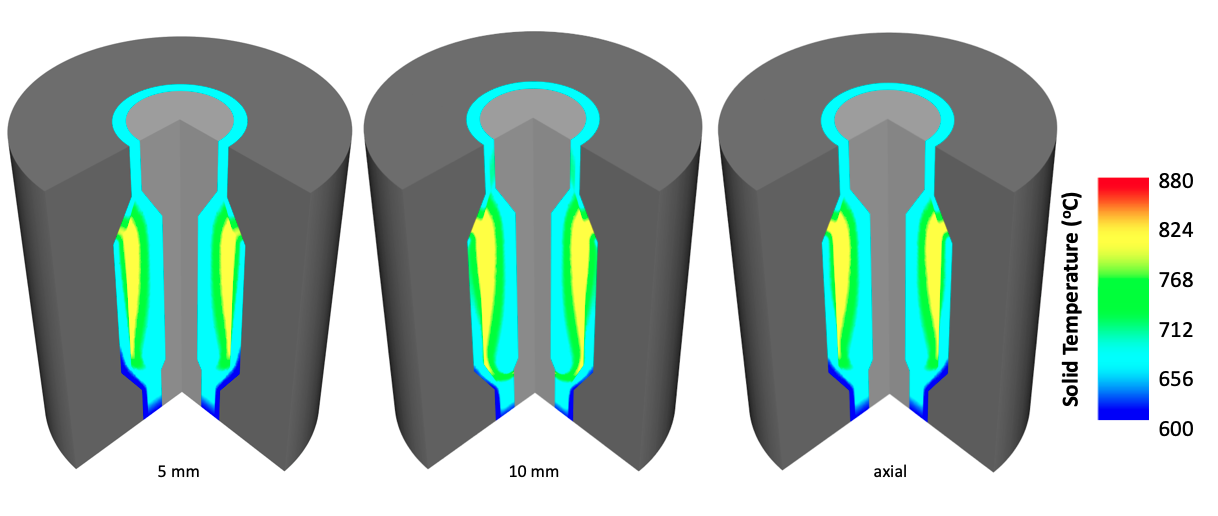
\includegraphics[height=0.4\linewidth]{figs/graphite.png}
\caption{Predicted average graphite temperature for inflow condition C$_\text{0.2}$ for all gap distributions.}
\label{fig:graphite}
\end{figure}

Similar to the fluid and solid temperature distributions shown in Figs. \ref{fig:fluid_temp_all}--\ref{fig:solid_noncore}, the coolant bypass from the core raises temperatures nearly uniformly through the bed. Table \ref{table:multiscale} summarizes the core maximum fluid temperature, maximum pebble surface temperature, maximum kernel temperature, and maximum of the average graphite as a function of outer reflector gap size. A maximum temperature is provided for the kernel to represent the proximity to individual-particle failure modes. Graphite forms many layers of the \glspl{cfp} as well as the matrix, shell, and inner core. Therefore, the maximum of the pebble-wise average graphite temperature, rather than the maximum graphite temperature, is provided as a more meaningful indication of pebble thermal conditions, such as potentials for fission product diffusion.

When the maximum fluid temperature is normalized to a common value for all three gap profiles, the temperature metrics shown in Table \ref{table:multiscale} are very similar. For instance, for all three gap distributions, the maximum pebble surface temperature is approximately 25\si{\celsius} higher than the maximum fluid temperature, the maximum average graphite temperature is approximately 25\si{\celsius} higher than the maximum pebble surface temperature, and the maximum kernel temperature is approximately 43\si{\celsius} higher than the maximum average graphite temperature. 

\begin{table}[htb!]
\caption{Predicted total bypass; maximum fluid, pebble surface, and UC$_{1.5}$O$_{0.5}$ temperatures; and maximum average graphite (``C '') temperature for inflow condition C$_{0.2}$ as a function of outer reflector gap size.}
\centering
\small
\centerline{
\begin{tabular}{|c |c| c c c c |}
\hline\hline
\multirow{2}{*}{Gap} & Total & Maximum & Maximum & Maximum & Maximum\Tstrut\\
 & Bypass (\%) & \(T_f\) (\si{\celsius}) & \(T_s\) (\si{\celsius}) & \(T_{\text{UC$_{1.5}$O$_{0.5}$}}\) (\si{\celsius}) & \(T_\text{C}\) (\si{\celsius})\Bstrut\\
 \hline
5 \si{\milli\meter} & 13.3 & 766.7 & 791.8 & 860.2 & 816.6\Tstrut\\
10 \si{\milli\meter} & 21.9 & 787.2 & 813.5 & 880.1 & 837.5\\
axial & 14.0 & 777.6 & 800.1 & 867.3 & 825.2\Bstrut\\
\hline
\end{tabular}
}
\label{table:multiscale}
\end{table}

Therefore, as already discussed in reference to the color plots of temperatures, the primary effect of the core bypass is to uniformly raise core temperatures. From the 5 \si{\milli\meter} gaps to the axial distribution, all temperatures increase by roughly 9\si{\celsius}, while from the axial distribution to the 10 \si{\milli\meter} gaps, all temperatures increase by a further 12\si{\celsius}. In order of increasing gap resistance, the maximum core temperatures decrease nearly linearly as less fluid is diverted through the reflector. However, it is interesting to note that the bypass fraction does not exhibit a similar linear trend. From the 5 \si{\milli\meter} gaps to the axial distribution, the bypass fraction increases by 0.007, while from the axial distribution to the 10 \si{\milli\meter} gaps, the bypass fraction increases by 0.079. This order of magnitude higher increase in the bypass does not directly translate to an order of magnitude higher increase in core temperatures, reinforcing the conclusion in Section \ref{sec:inflow} that the effect of the bypass fraction on core temperatures is a nonlinear function of operating conditions and flow \glspl{bc}. 

While a multi-dimensional, unstructured-mesh application such as Pronghorn can capture the cross-flow effects between the bed and the reflectors, it is difficult to condense such effects into a single measurement of the bypass fraction. Slightly different conclusions may transpire with different definitions of the bypass fraction.
% this feels unsatisfactory, can you elaborate a little bit? This seems like a summary of a lot of what you've been showing and hammering it home a little seems useful. 

At each computational element in the bed, the \gls{hsd} model is used to compute integral temperature solutions that were shown for the kernel and graphite in Figs. \ref{fig:uo2_max}--\ref{fig:graphite}. To provide additional elaboration on the \gls{hsd} model application to the \gls{pbfhr}, the left half of Fig.\ \ref{fig:multiscale_fuel} shows the pebble surface temperature with solid black contour lines for the 5 \si{\milli\meter} gap distribution. This data is also shown in Fig.\ \ref{fig:solid_core} on a shared color scale for all three gap distributions. Throughout the bed, nine equally-spaced axial positions are indicated with horizontal dashed lines. The axially-symmetric sinusoidal power distribution results in the same pebble power density at \(z=0.53\) and 4.78 \si{\meter}, at \(z=1.06\) and 4.25 \si{\meter}, at \(z=1.59\) and 3.72 \si{\meter}, and at \(z=2.13\) and 3.19 \si{\meter}.

On each horizontal line, a colored circle indicates the location of the maximum UC$_{1.5}$O$_{0.5}$ temperature on that line. Because the sinusoidal power distribution only contains an axial dependence, the maximum UC$_{1.5}$O$_{0.5}$ temperature location coincides with the maximum pebble surface temperature location. In the right half of Fig.\ \ref{fig:multiscale_fuel}, the meso and micro scale temperature distributions are shown at the nine axial positions at the maximum kernel temperature location. The mesoscale temperature represents the long-wavelength heat conduction solution due to the homogenized heat source and thermal properties, while the mesoscale temperature represents a small-scale correction associated with a localized heat source and heterogeneous \gls{cfp} thermal properties. 

\begin{figure}[h!]
\centering
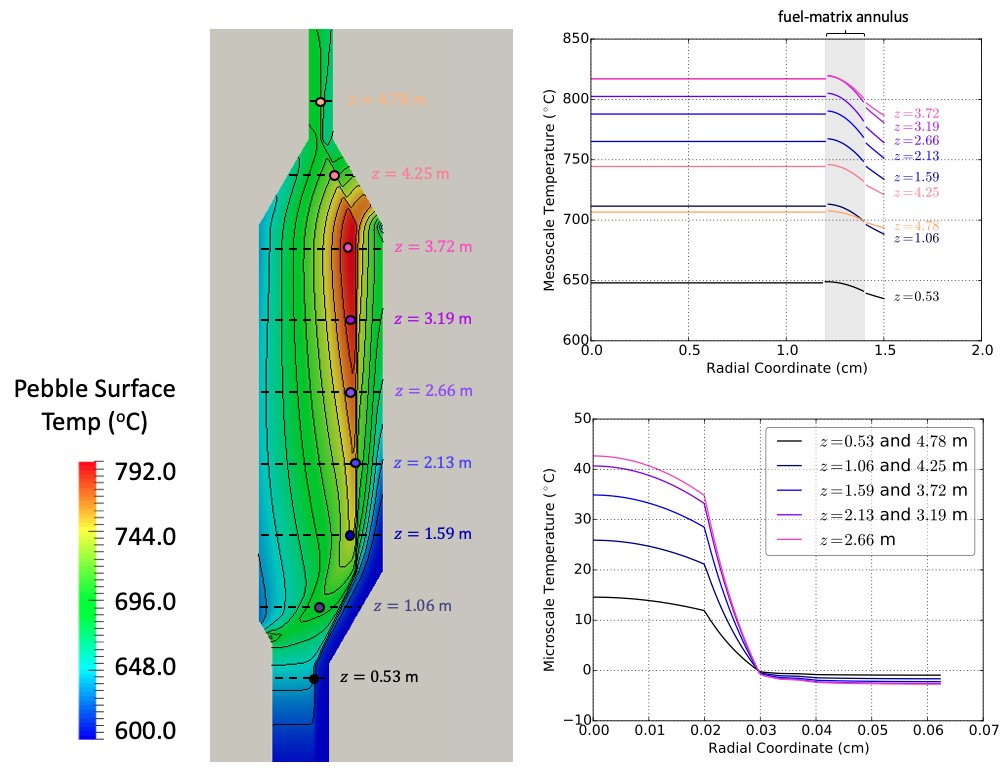
\includegraphics[width=0.9\linewidth]{figs/multiscale_fuel.png}
\caption{Predicted pebble surface temperature (left) and meso and micro scale temperatures (right) for inflow condition C$_\text{0.2}$ for the 5 \si{\milli\meter} gap distribution. }
\label{fig:multiscale_fuel}
\end{figure}

Because the locations of the \glspl{cfp} within each \gls{pbfhr} pebble are unknown, the meso and micro scale temperatures are shown on separate plots rather than summed together as in Eq. \eqref{eq:MultiscaleSolution}. The maximum and average temperatures shown in Figs. \ref{fig:uo2_max}--\ref{fig:graphite} are evaluated with the approximations in Eqs. \eqref{eq:MaxT} and \eqref{eq:AvgT}, respectively. Discontinuities exist between the fuel-matrix temperature and the homogeneous core and shell temperatures in the mesoscale solution because it is only the sum of the meso and micro scale solutions that satisfy continuity in temperature and heat flux with neighboring regions.

Most of the mesoscale temperature drop occurs over the fuel-matrix annulus. The lack of a volumetric heat source, combined with the uniform pebble surface \gls{bc}, results in uniform temperatures in the inner core region. Moving from the bottom of the bed to the top, the pebble surface temperature increases as the fluid temperature rises by convective heat transfer. It is the combination of a high surface temperature with a high power density that results in the highest kernel temperatures occurring in the upper half of the bed, about 1 \si{\meter} above the axial mid-plane.

Because the surface \gls{bc} in the microscale domain is independent of the pebble surface temperature, the microscale solution is only dependent on the pebble power density. Therefore, the nine unique axial positions collapse into five microscale temperature distributions corresponding to the five unique power densities. With properties and geometry fixed, the maximum kernel temperature in the microscale solution is directly related to the power density. Most of the microscale temperature drop occurs across the low-conductivity porous buffer layer. While virtually all porous graphite thermal properties are quoted as constant in the literature \cite{sun,tecdoc1694,xin_wang_thesis,stainsby,parfume,hales,rochais,lopez_honorato}, small absolute changes in thermal conductivity associated with fission product gas accumulation or other irradiation-induced degradations may have a large effect on maximum temperature predictions, and are worthy of future study.

\section{Summary and Conclusions}
\label{sec:conclusions_fhr}

The high volumetric heat capacity and high boiling point of molten salts have in the past 20 years led to considerable interest in the use of salt coolants for \glspl{pbr}. Essential to the development of a general-purpose, single-phase \gls{pbr} \gls{th} simulation tool is demonstration for a wide range of systems. In lieu of an experimental validation similar to that performed for gas coolants in Chapter \ref{sec:sana}, this section applied the multiscale models in Chapter \ref{sec:PhysicalModels} to the \gls{pbfhr}, a \gls{flibe}-cooled \gls{pbr} under development by the Nuclear Engineering Department at \gls{ucb}.

The \gls{pbfhr} design differs from gas-cooled \glspl{pbr} in several important areas, motivating the exploratory investigations performed in this chapter. Though the \gls{pbfhr} \gls{cfp} design is based on the standard \gls{triso} particle, the fuel-matrix region of the \gls{pbfhr} fuel pebbles is only 0.2 \si{\centi\meter} thick, or about 2.5 \glspl{cfp} wide. For comparison, the fuel-matrix core of the \gls{htr10} pebble is 5 \si{\centi\meter} thick, or about 55 \glspl{cfp} wide. This factor of about 20 difference in thermal ``thickness'' required verification of the \gls{hsd} and \gls{hl} methods for the \gls{pbfhr} fuel design.

In Section \ref{sec:meso_fhr}, the \gls{hsd} and \gls{hl} model predictions were compared against reference, fully-resolved, fuel pebble heat conduction for a range of pebble thermal conditions. The \gls{hsd} model predicts material-wise average and maximum temperatures to within 10\si{\celsius} over a wide range in particle \gls{pf}, demonstrating both the robust nature of the \gls{hsd} model to variations in pebble design and its applicability to the nominal \gls{pbfhr} design. Conversely, the \gls{hl} method exhibits non-physical trends with \gls{pf} and generally fails to predict integral temperatures due to an inability to preserve the particle thermal resistance at low \glspl{pf}. At low \glspl{pf}, where the \gls{hsd} error in the maximum kernel temperature is only on the order of 10\si{\celsius}, the \gls{hl} method is characterized by errors in excess of 200\si{\celsius}. Recent transient studies of the \gls{pbfhr} with the \gls{hl} model \cite{xin_wang_thesis} should be repeated with the more accurate \gls{hsd} model to reevaluate proximity to thermal limits and Doppler broadening negative temperature feedback.

Predicting core bypass flows has been identified as an important area in simulation tool development for gas-cooled \glspl{pbr} \cite{gou_2018}. Bypass flows divert coolant from the fuel, resulting in higher fuel and coolant temperatures that reduce margins to \gls{cfp} and structural material failure and other complications such as excessive forces in defueling chutes. Bypass flow is expected to play an equivalently important role in salt-cooled \glspl{pbr}, but to the author's knowledge, no studies have attempted to quantify the bypass fraction in the \gls{pbfhr} \cite{pbfhr_website}.

Full-core resolved \gls{cfd} modeling of the \gls{pbfhr} outer reflector system is beyond reach of the computing resources available for this work. Based on the multiscale concept applied to the pebble bed region, this work models the outer reflector blocks as a porous media with macroscale closures obtained from the literature. The presence of both horizontal and vertical machined flow channels in the \gls{pbfhr} outer reflector block results in stronger axial and radial coupling than in prototypic gas-cooled reflector blocks, precluding the utilization of existing gas-cooled \gls{pbr} reflector block friction factor correlations. 

In Section \ref{sec:bypass}, anisotropic drag models were correlated with COMSOL Multiphysics \gls{cfd} simulations of half- and quarter-size blocks as a function of Reynolds number and block gap size. Uniform gap widths of 5 and 10 \si{\milli\meter} were considered. These fairly large gaps were selected to bound the maximum bypass fraction expected over a lifetime of temperature- and irradiation-induced dimensional changes in the reflector blocks. A significant number of simplifying geometric and model assumptions were made in this analysis. Grooves on the block faces were neglected for ease of incorporating dimensional changes, while braided carbon fiber tubing was not considered due to insufficient characterization in the available design documents. Uniform gaps neglect the dependence of deformation on fast fluence, which is significantly higher in the 10 to 20 \si{\centi\meter} facing the bed. Further, uniform horizontal gaps result in block rings floating relative to one another; while the graphite reflectors are nearly neutrally-buoyant in the \gls{flibe} coolant, the horizontal gaps are more similar to wedges than prisms. In the absence of deformation block measurements for the \gls{pbfhr}, these simplified geometries should be understood as coarse approximations to the true block geometry. Because the gap widths are likely smaller than 5 \si{\milli\meter} in lower-fluence regions, these simplified geometries are in line with the present objective of bounding the maximum bypass fraction.
% any comments about what some of these approximations might mean? e.g. more fast fluence would do x so we might expect more y in 10-20 cm facing the bed. This helps us understand the results. Maybe just stating why all of the simplifications support that this is a bound would be helpful. 

From a more fundamental perspective, the pressure gradient was correlated in terms of a diagonal tensor with coefficients obtained from isolated simulations of flow in mutually orthogonal directions. Experiments are required to quantify the accuracy of this decomposition for the particular geometry considered.

The one-equation Spalart-Allmaras turbulence model is used due to limited computational resources and the substantial geometric simplifications already made. By modeling a single reflector block, flow development effects were not considered. For the vertical flow cases in particular, imposing a uniform mass flux on the inlet faces is a simplification of the actual flow distribution that would be more heavily concentrated near the vertical coolant channel. The reduction in directional changes expected when considering multiple stacked blocks will likely reduce the friction factors in the axial direction, increasing flow through the outer reflector.

The \gls{bc} imposed at the bed-reflector interface should also account for the randomly-heaped pebble geometry, which has a significant effect on the flow distribution in this region \cite{amini}.
% Does it? Which ones do? I'm not sure what the "should" here means. 
Future work will repeat the \gls{cfd} correlation of outer reflector block friction factors with a two-equation turbulence model for multiple stacked blocks adjacent to a resolved pebble bed.

The \gls{cfd} pressure drop predictions for 5 and 10 \si{\milli\meter} gaps were correlated as friction factors for the radial and axial flow directions. While only two gap sizes were considered, it is clear that the gap width has a significant effect on the drag. By decreasing the gap width from 10 to 5 \si{\milli\meter}, the friction factor on average increases by 105.\% and 125.7\% for the radial and axial directions, respectively. The friction factor is also very dependent on the flow direction with the radial friction factor 151.8\% and 176.3\% higher than the axial friction factor at gap sizes of 5 and 10 \si{\milli\meter}, respectively. 

In Section \ref{sec:core}, the multiscale model described in Chapter \ref{sec:PhysicalModels} was combined with the \gls{hsd} verification in Section \ref{sec:meso_fhr} and the reflector \gls{cfd} drag modeling in Section \ref{sec:bypass} for full-core steady-state analysis of the \gls{pbfhr}. In Section \ref{sec:inflow}, five different inner reflector \glspl{bc} were considered in conjunction with three different reflector block gap distributions to 1)~investigate how the inlet flow \gls{bc} affects the fluid temperature distribution and bypass fraction and 2)~recommend an inlet \gls{bc} that achieves a balance between minimizing the bypass fraction, maximum and average fluid temperature on the plenum inlet, and core pressure drop.

For all \glspl{bc} and gap distributions considered, a net flow of coolant from the outer reflector into the pebble bed exists, primarily along the bottom angled surface of the outer reflector. The core pressure drop is fairly insensitive to the gap size and inflow condition, though \glspl{bc} with a lower ``center of mass flux'' exhibit higher pressure drops because of the longer fluid path length through the bed.

The inflow \gls{bc} has a significant effect on the bypass and outlet fluid temperature distribution. For a fixed gap distribution, varying the inflow \gls{bc} results in roughly a 0.025 range in bypass fraction, a 15\si{\celsius} range in the average plenum inlet temperature, and a 95\si{\celsius} range in the maximum plenum inlet temperature. Generally, a higher reflector block resistance results in a lower bypass and lower core temperatures, but comparisons among multiple \glspl{bc} show that the bypass fraction alone is not the sole indicator of the maximum and average fluid temperature along the inlet plenum. %what else do we need to consider? How important are those things relative to one another?

By balancing the core pressure drop, maximum coolant outlet temperature, and range in coolant outlet temperature, an inlet \gls{bc} more heavily weighted towards the bottom of the bed is recommended as a starting point for further design studies. For this particular \gls{bc}, if the 5 \si{\milli\meter} uniform gaps or the sinusoidal interpolation between 5 and 10 \si{\milli\meter} gap distributions are representative of reflector block end-of-life conditions, the core bypass fraction is estimated to be in the range of 13.3--15.4\%, depending on how the bypass is defined. The similarity in the bypass fraction for the uniform 5 \si{\milli\meter} and axial gap distributions implies that the bypass fraction is strongly affected by the block drag near the extremities of the bed. A different block design in these regions may allow greater control over the core bypass fraction.

In Section \ref{sec:depth}, in-depth \gls{th} predictions for the three reflector gap distributions were shown for the optimized inflow condition. Because core bypass diverts coolant from the entirety of the bed, a higher bypass raises core temperatures nearly uniformly through the bed. Fluid, pebble surface, kernel, and graphite temperatures for the three gap distributions differ from one another primarily in magnitude. Averaged over the various gap distributions, the maximum average graphite temperature and maximum kernel temperature are approximately 25\si{\celsius} higher and 68\si{\celsius} higher, respectively, than the pebble surface temperature. While differences in hundreds of degrees between peak and surface fuel temperatures are common in \glspl{lwr} and gas-cooled \glspl{pbr}, the close proximity of the \glspl{cfp} to the pebble surface result in relatively small fuel temperature gradients in the \gls{pbfhr} design. 

Project timelines restricted the \gls{cfd} modeling to prediction of friction factor closures for the outer reflector blocks. The complex inner and outer reflector block geometries precluded the use of existing convective heat transfer closures, so convective heat transfer was neglected in the reflectors. Therefore, fluid temperatures in the outer reflector are underpredicted, while reflector temperatures are overpredicted. Because the highest fluid temperatures occur in the pebble bed region, where convective heat transfer is considered, this modeling simplification is likely conservative from the perspective of peak temperatures. Further, the use of a sinusoidal heat source to decouple the thermal analysis from neutron transport neglects radial power peaking \cite{xin_wang_thesis}. For the axial power distribution assumed in this work, the highest kernel temperatures were observed at the interface between the fuel and blanket pebbles, where power peaking may result in even higher temperatures.

A number of important geometric design details for the \gls{pbfhr} are either lacking or insufficiently characterized, requiring several assumptions in the construction of a computational model of the reactor that may also affect the applicability of the predictions in this chapter to the nominal \gls{pbfhr} design. Insufficient details for the inlet plenum design, combined with the desired flexibility in specifying the inlet flow \gls{bc}, motivated modeling the inner reflector as a solid conducting slab mixture of \gls{flibe} and graphite. And, even though the outer reflector block geometry varies with height because of the conical fueling and defueling regions, the same drag closures were used throughout. Future work will refine the geometry and closures in the computational model and revisit the predictions made in this chapter.

The primary objective of this section is to apply the models in Chapter \ref{sec:PhysicalModels} to a salt-cooled \gls{pbr} with a design that differs significantly from the gas-cooled concepts that have dominated the assessment of multiscale thermal models for \glspl{pbr}. The multi-dimensional core flow and the interaction of the bed with the angled outlet is easily accounted for with the unstructured meshing capabilities available with \gls{moose}-based applications. A large suite of macroscale closures allows the inclusion of radiation and pebble contact conduction physics that have been neglected in most previous models of the \gls{pbfhr}. Importantly, the \gls{th} models implemented in Pronghorn are just one component in a comprehensive \gls{moose}-based reactor analysis framework. Ongoing work at \gls{inl} in the areas  of multiphysics coupling to neutron transport, systems-level \gls{th}, and fuels performance will expand the multiscale models described in this work to more complex analysis and transients relevant to advanced reactor design.
